\part{Efeito dos aditivos hidrofílicos}
	
	Esta é a parte principal desta tese, onde a maior parte do tempo foi dedicada ao entendimento dos efeitos dos aditivos hidrofílicos no comportamento das micelas gigantes. Os resultados foram publicados na revista \emph{Journal of Colloid and Interface Science}, sob o título ``\emph{Rheological and calorimetric study of alkyltrimethylammonium bromide-sodium salicylate wormlike micelles in aqueous binary systems}".
	
	Serão apresentados inicialmente os resultados reológicos em função do efeito dos aditivos, e em seguida serão levantados alguns parâmetros que podem ser utilizados para descrever o efeito dos aditivos.
	
	Inicialmente, escolheu-se sacarose pois possui tipos de interação semelhantes à glicerina, e já havia sido testada em outros sistemas como, por exemplo, sistemas lamelares, onde teve o mesmo efeito da glicerina. 1,3-butanodiol (1,3BD) foi um aditivo escolhido devido a um estudo feito por Rami Abdel-Rahem, e seu estudo foi reproduzido e complementado com informações calorimétricas. Dimetilsulfóxido (DMSO) também é utilizado na literatura como um aditivo. A ureia é um aditivo que é frequentemente descrito na literatura como um agente desestruturante da água, que leva à desnaturação de proteínas.
	
	% todo: encontrar o motivo para DMSO.
	
	\chapter{Resultados}
		\section{Efeitos dos aditivos na reologia}
			
			A reologia é uma técnica que pode fornecer informações sobre a dinâmica de relaxação de um material, através da viscosidade. Em especial, o perfil de viscosidade em repouso (\(\eta_0\)) em função da concentração de cossoluto está relacionado com mudanças no processo de relaxação das micelas. Com o intuito de se estudar como a relaxação das micelas é afetado pelos aditivos, foram construídos vários diagramas de viscosidade em função da concentração de salicilato de sódio.
			
			Dos cinco aditivos selecionados, foram feitas comparações para realçar as diferenças e semelhanças entre os aditivos. Neste momento, os resultados serão discutidos com base somente no índice de refração das soluções. A figura \ref{fig:indice_refracao} mostra como o índice de refração das soluções com os aditivos variam em função da fração mássica de aditivo.
					
			\begin{figure}[h]
				\centering
				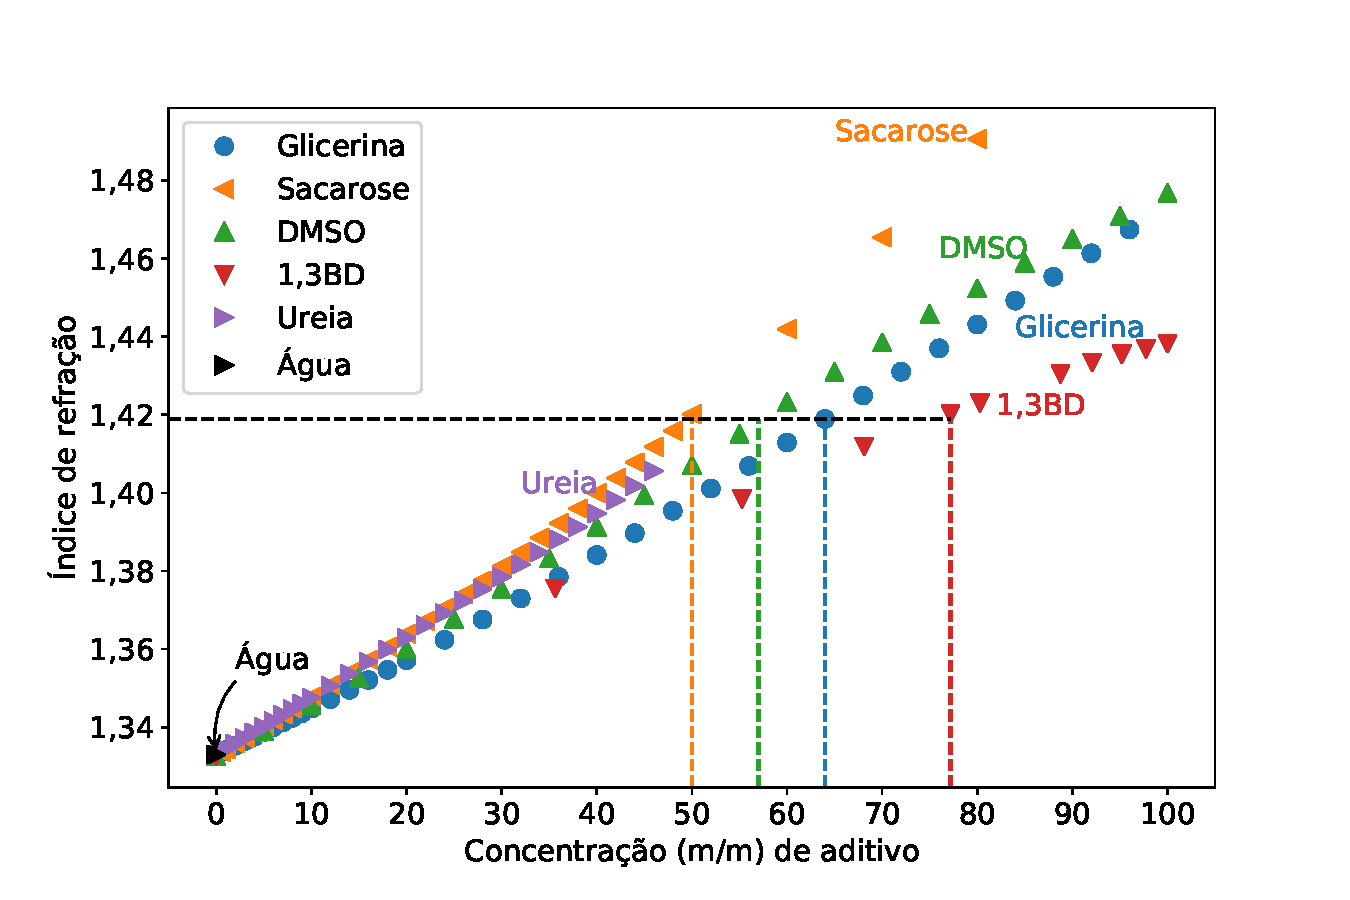
\includegraphics[width=0.7\textwidth]{imagens/propriedades/indice_refracao}
				\caption{Índice de refração em função da concentração de aditivo}
				\label{fig:indice_refracao}
			\end{figure}
	
			Inicialmente, comparou-se o sistema melhor estudado (glicerina) com sacarose, escolhida pois também possuía efeitos semelhantes à glicerina no intumescimento lamelar. A figura \ref{fig:rh_sacarose_glicerina} mostra os diagramas de viscosidade para soluções de micelas gigantes com 100 \mM{} de \CTAB, em concentrações crescentes de glicerina, e no ponto de igualdade no índice de refração de sacarose, 50\%.
			
			\begin{figure}[h]
				\centering
				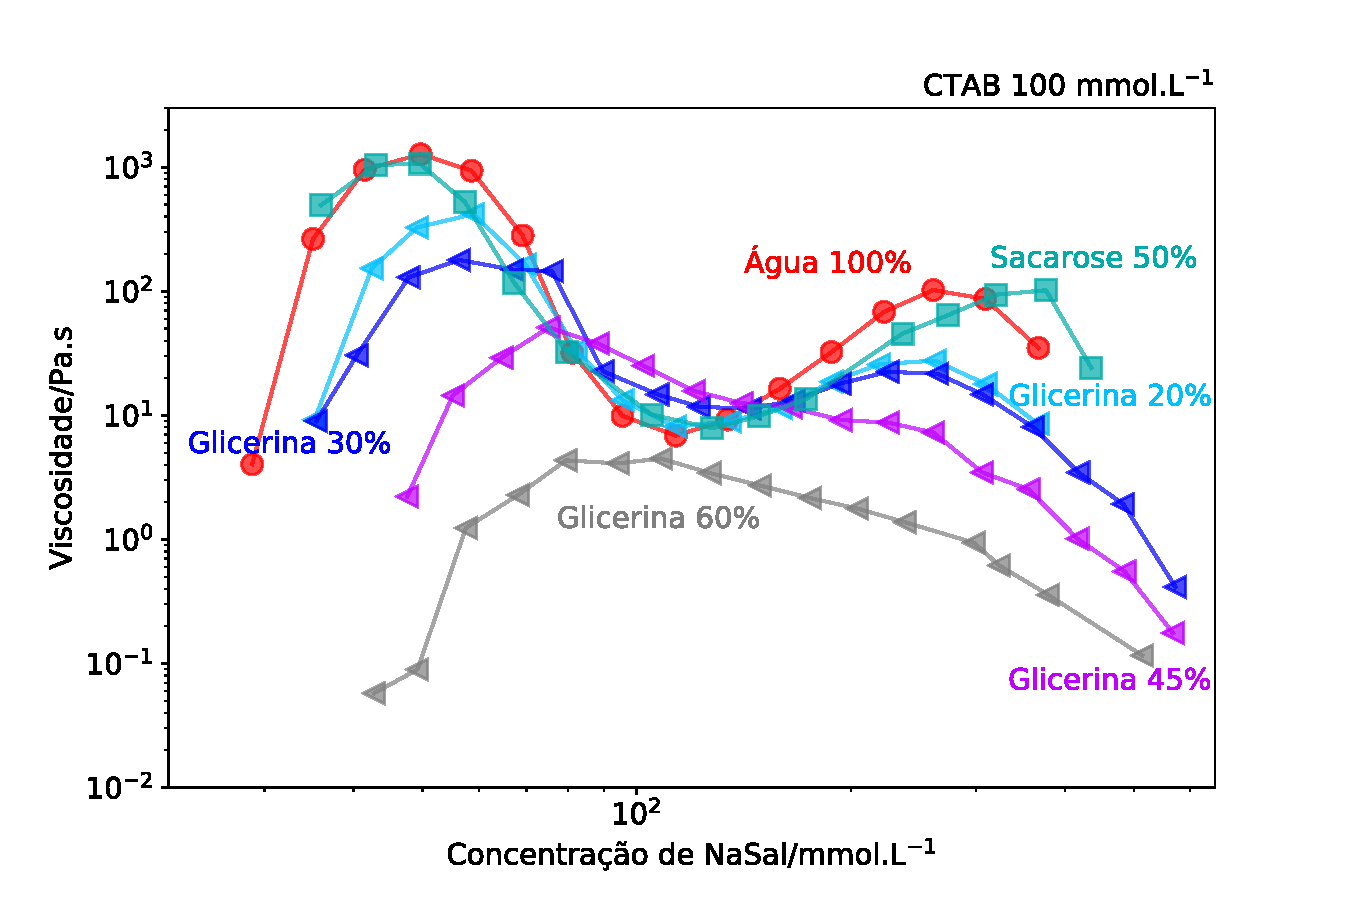
\includegraphics[width=0.7\textwidth]{imagens/reologia/RH_sacarose_glicerina}
				\caption{Viscosidade no repouso \(\eta_0\) em função da concentração de salicilato de sódio (NaSal) em várias concentrações dos aditivos glicerina e sacarose. 60\% de glicerina (V/V) e 50\% de sacarose (m/m) estão no ponto de equivalência do índice de refração.}
				\label{fig:rh_sacarose_glicerina}
			\end{figure} % todo: mencionar que curvas a laila mediu. Foram as de glicerina?
			
			Podemos observar que os dois picos de viscosidade observados em pequenas concentrações de glicerina, diminuem, e a região central permanece pouco afetada, como já havia sido descrito por Hoffmann. Porém, vemos que a adição de 50\% de sacarose praticamente não afetou a viscosidade das soluções, apesar da igualdade no índice de refração dessas soluções. Isso mostra que considerar somente o índice de refração não permite a previsão do comportamento dessas soluções, e isso motivou a realização de estudos posteriores.
			
			A figura \ref{fig:rh_13bd_dmso} mostra como os aditivos 1,3-butanodiol e dimetilsulfóxido afetam o perfil de viscosidade.
			
			\begin{figure}[h]
				\centering
				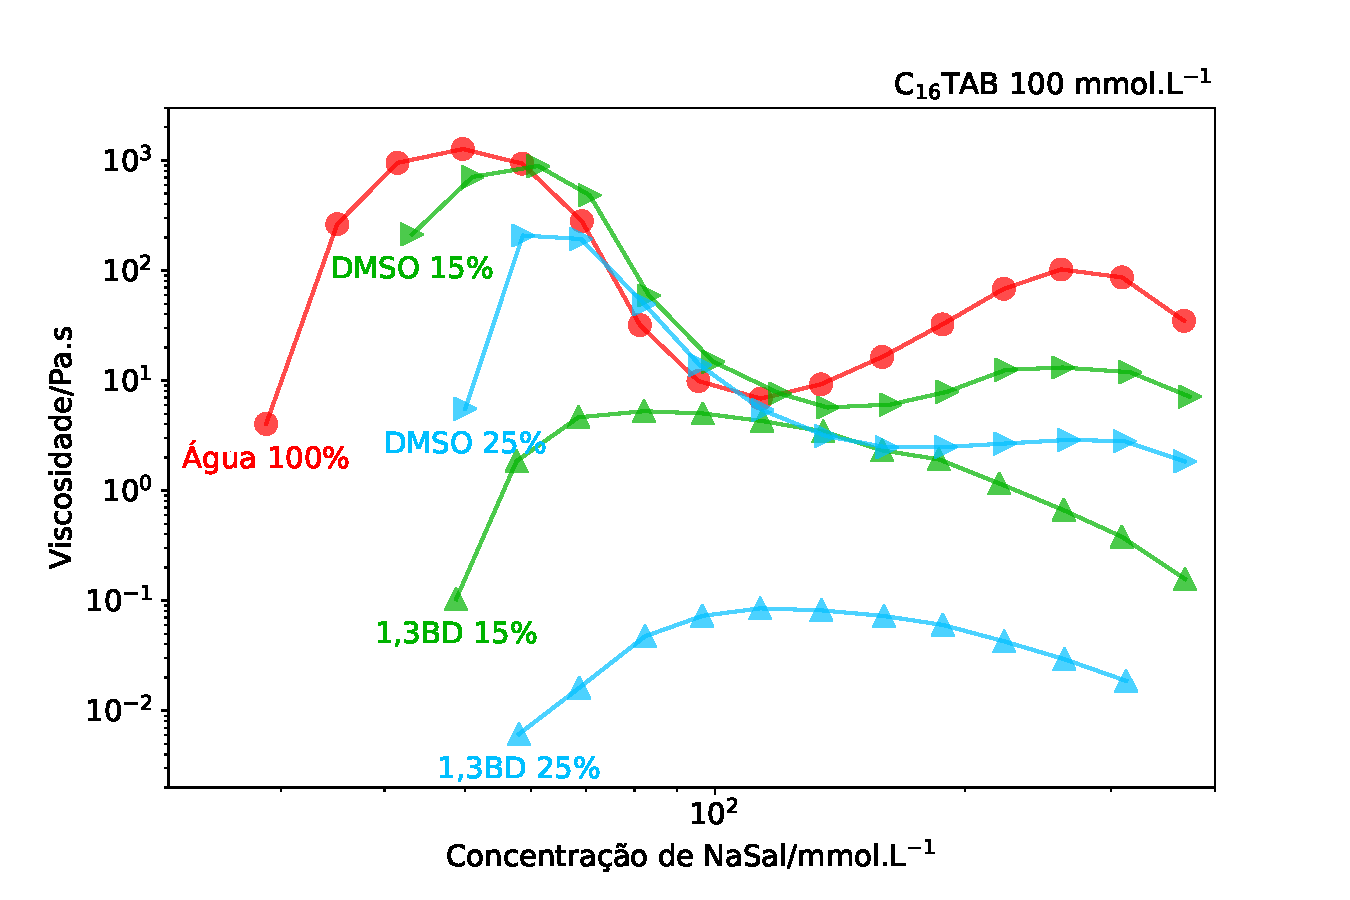
\includegraphics[width=0.7\textwidth]{imagens/reologia/RH_13BD_DMSO}
				\caption{Viscosidade no repouso \(\eta_0\) em função da concentração de salicilato de sódio (NaSal) em várias concentrações dos aditivos 1,3-butanodiol (1,3BD) e dimetilsulfóxido (DMSO). As concentrações de igualdade do índice de refração são 77\% (m/m) e 57\% (m/m), respectivamente}
				\label{fig:rh_13bd_dmso}
			\end{figure}
		
			O perfil de viscosidade dessas soluções foi muito mais afetado pelos aditivos do que era esperado observando-se somente o índice de refração, em especial o 1,3-butanodiol, onde 15\% (m/m) possui o mesmo efeito na viscosidade que 60\% de glicerina.
			
			A ureia possui o comportamento que mais difere dos outros aditivos, como mostra a figura \ref{fig:rh_ureia}.
			
			\begin{figure}[h]
				\centering
				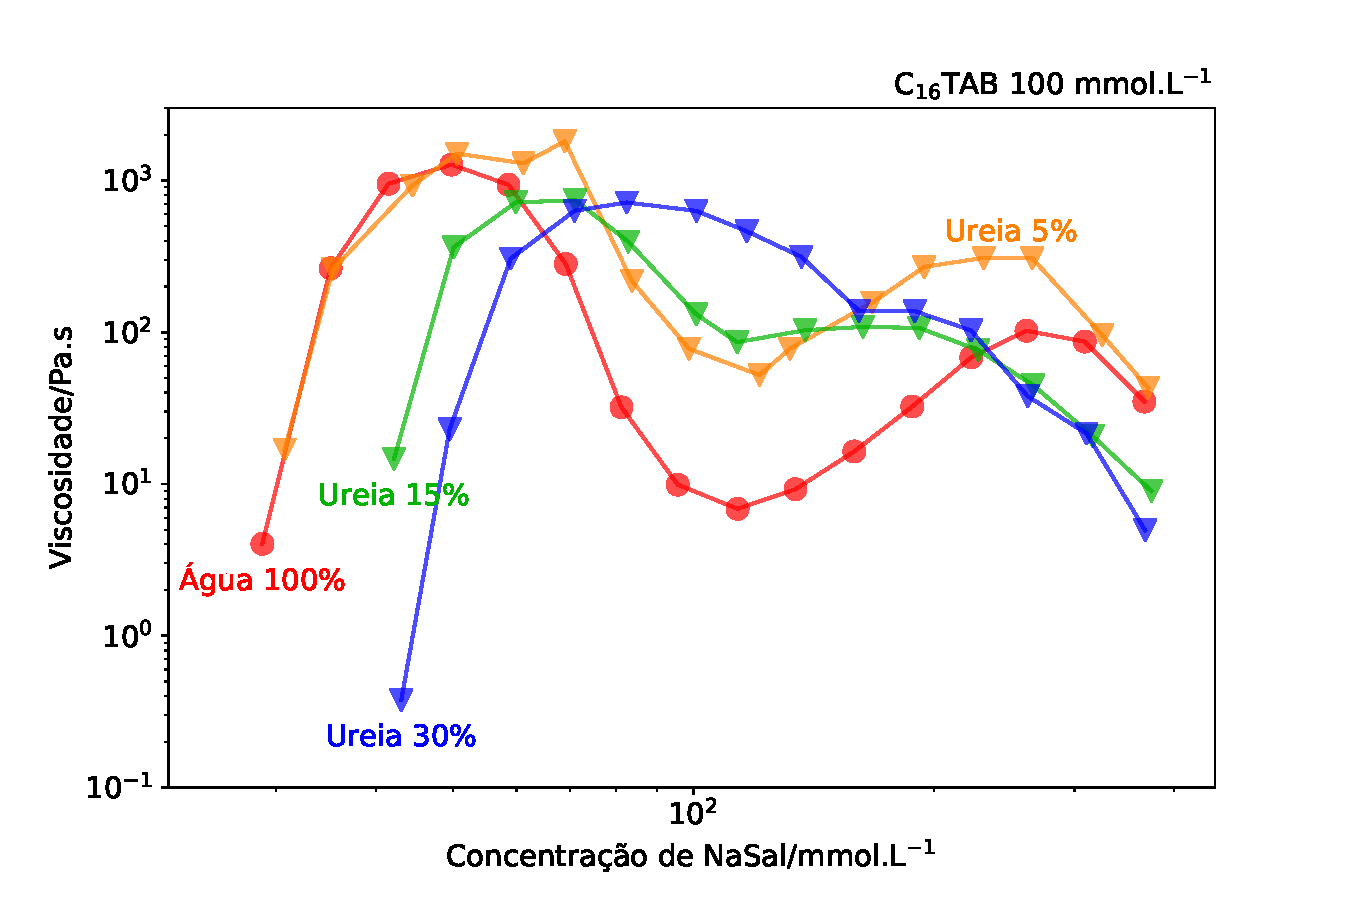
\includegraphics[width=0.7\textwidth]{imagens/reologia/RH_ureia}
				\caption{Viscosidade no repouso \(\eta_0\) em função da concentração de salicilato de sódio (NaSal) em várias concentrações de ureia. A concentração de igualdade de índice de refração é em torno de 55\%.}
				\label{fig:rh_ureia}
			\end{figure}

			Nesse caso, a viscosidade na região central aumentou, algo não observado nos outros cossolutos. Outro caso que possui um comportamento semelhante é o diagrama de orto-hidróxicinamato e \CTAB{} em pH 9. %todo: citar o artigo do OHCA
		
		\FloatBarrier
		
		\section{Efeito dos aditivos na calorimetria de micelas gigantes}
		
			A calorimetria de titulação isotérmica fornece informações sobre o quão favorável é a formação das micelas, através da concentração de formação de micelas gigantes, \cwlm. As figuras \ref{fig:itc_mg_glicerina} -- \ref{fig:itc_mg_ureia} mostram os perfis de formação de micelas gigantes para glicerina, sacarose, 1,3-butanodiol, dimetilsulfóxido e ureia.
		
			\begin{figure}[h]
				\centering
				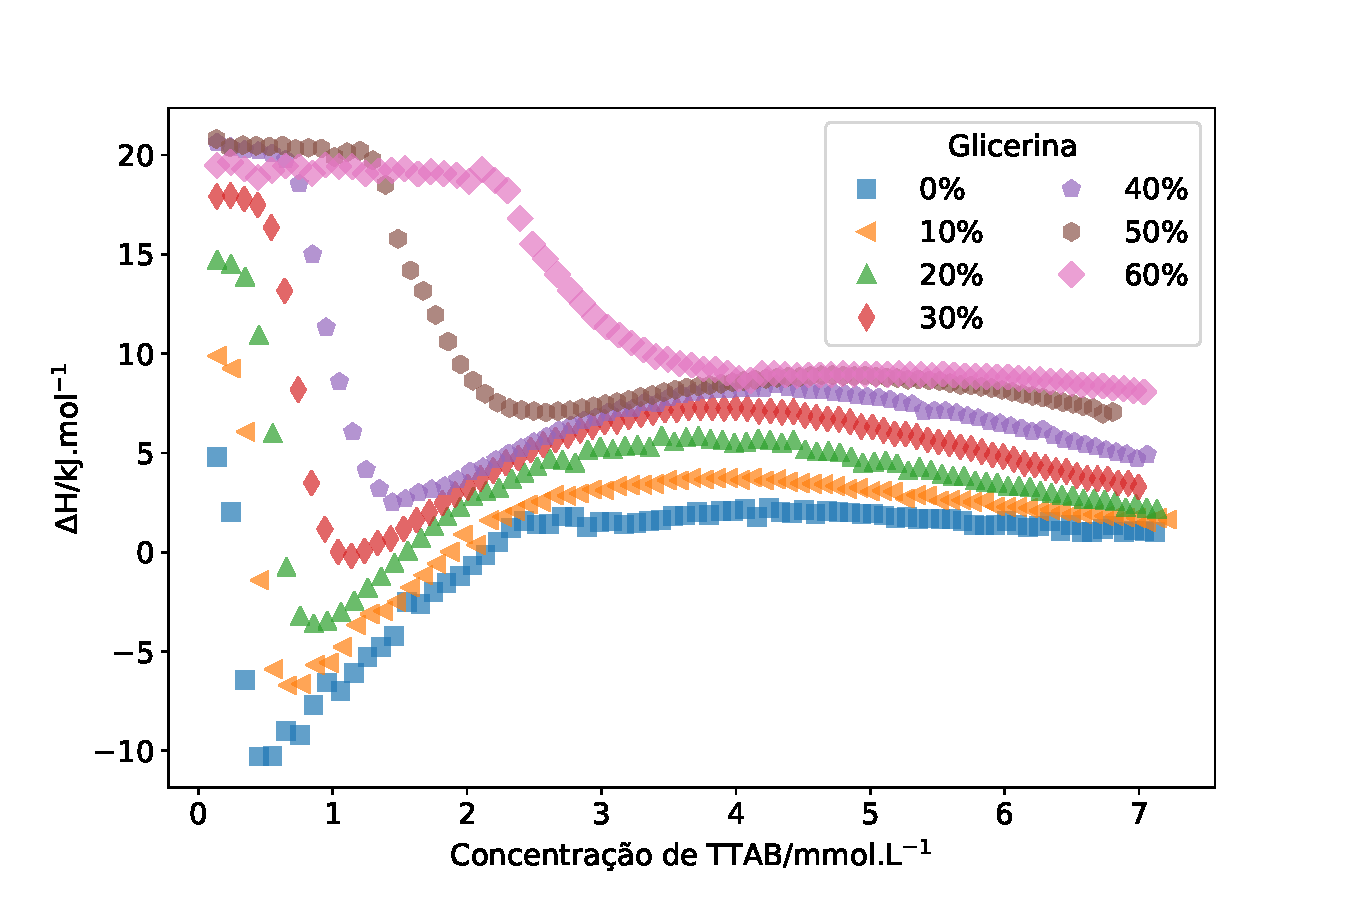
\includegraphics[width=0.7\textwidth]{imagens/itc/ITC_MG_glic}
				\caption{Efeito da concentração de glicerina nas curvas de titulação de formação de micelas gigantes. A concentração de salicilato de sódio na cela de amostra é de 1,5\mM. A concentração do aditivo está em \% (V/V).}
				\label{fig:itc_mg_glicerina}
			\end{figure}  % todo: colocar a curva sem aditivo em todos. Trocar o 0% por uma curva preta.
			
			\begin{figure}[h]
				\centering
				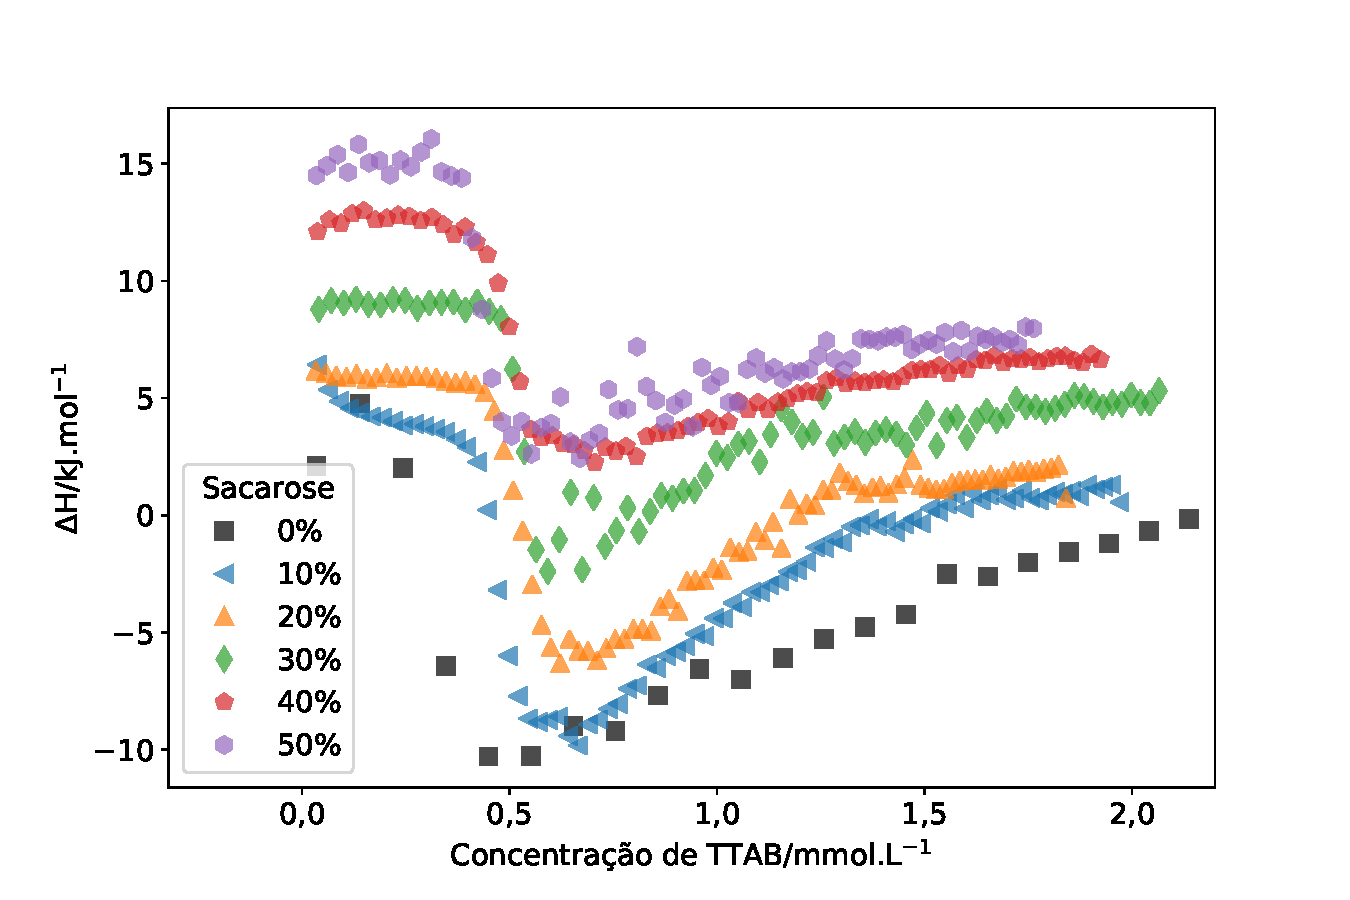
\includegraphics[width=0.7\textwidth]{imagens/itc/ITC_MG_sac}
				\caption{Efeito da concentração de sacarose nas curvas de titulação de formação de micelas gigantes. A concentração de salicilato de sódio na cela de amostra é de 1,5\mM. A concentração do aditivo está em \% (m/m).}
				\label{fig:itc_mg_sacarose}
			\end{figure}
			
			As diferenças entre glicerina e sacarose, novamente, se evidenciaram. Da mesma maneira que na reologia, a presença de sacarose não afetou a formação de micelas gigantes. Já a glicerina teve um efeito deletério, aumentando significativamente a concentração necessária para o crescimento.
						
			\begin{figure}[h]
				\centering
				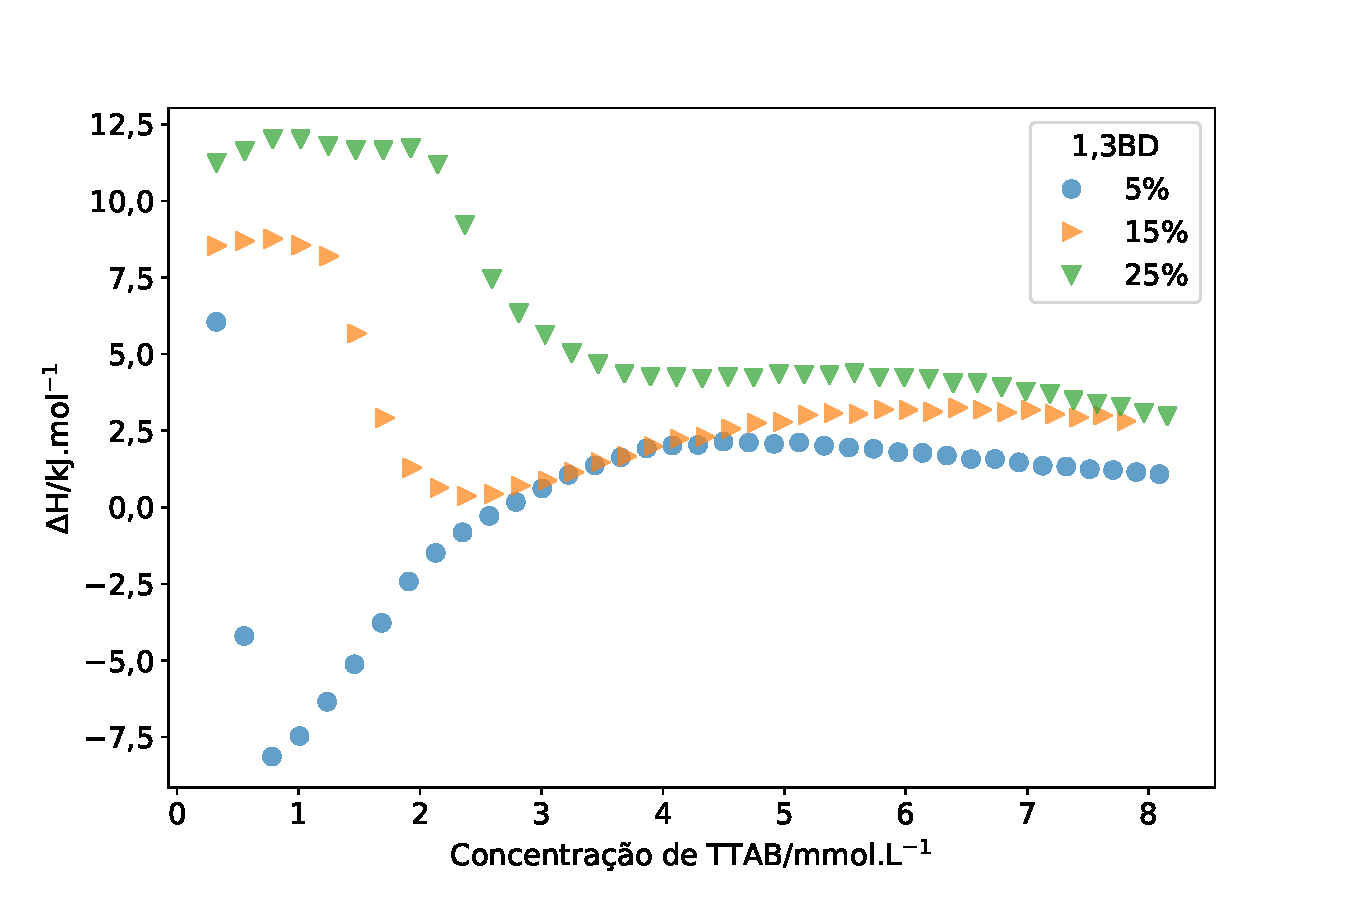
\includegraphics[width=0.7\textwidth]{imagens/itc/ITC_MG_13BD}
				\caption{Efeito da concentração de 1,3-butanodiol nas curvas de titulação de formação de micelas gigantes. A concentração de salicilato de sódio na cela de amostra é de 1,5\mM. A concentração do aditivo está em \% (m/m).}
				\label{fig:itc_mg_13bd}
			\end{figure}
			
			\begin{figure}[h]
				\centering
				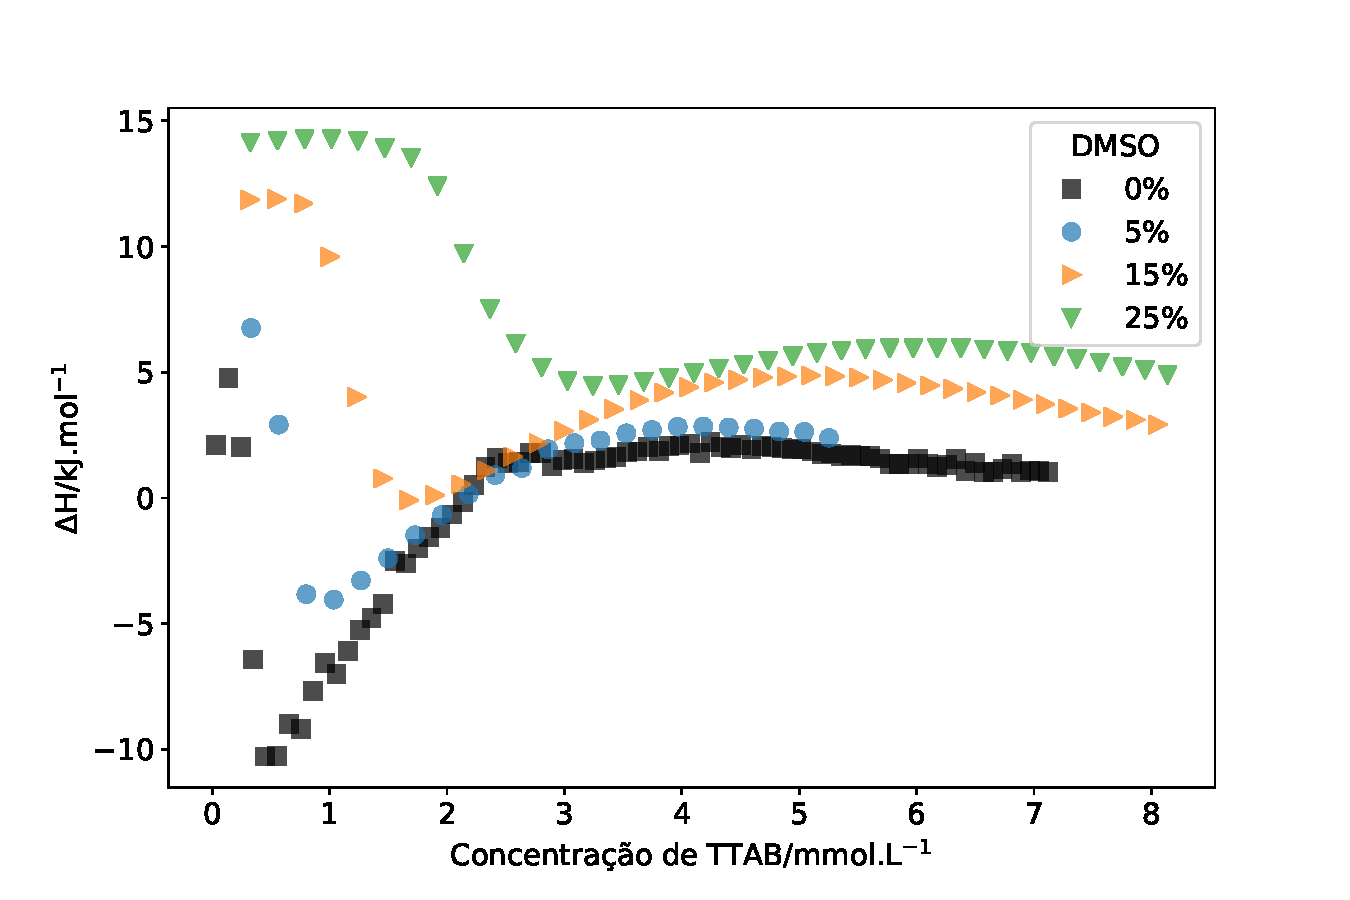
\includegraphics[width=0.7\textwidth]{imagens/itc/ITC_MG_dmso}
				\caption{Efeito da concentração de dimetilsulfóxido nas curvas de titulação de formação de micelas gigantes. A concentração de salicilato de sódio na cela de amostra é de 1,5\mM. A concentração do aditivo está em \% (m/m).}
				\label{fig:itc_mg_dmso}
			\end{figure}  % todo: será que dá pra juntar os dois?

			1,3-BD e DMSO não se mostraram muito diferentes, apesar dos perfis reológicos serem bastante distintos, algo não totalmente inesperado, já que ambas as técnicas observam fenômenos diferentes. Isso indica que a queda de viscosidade com 1,3-BD não se deve à uma desestabilização micelar, o que levaria à uma diminuição na quantidade de micelas.

			\begin{figure}[h]
				\centering
				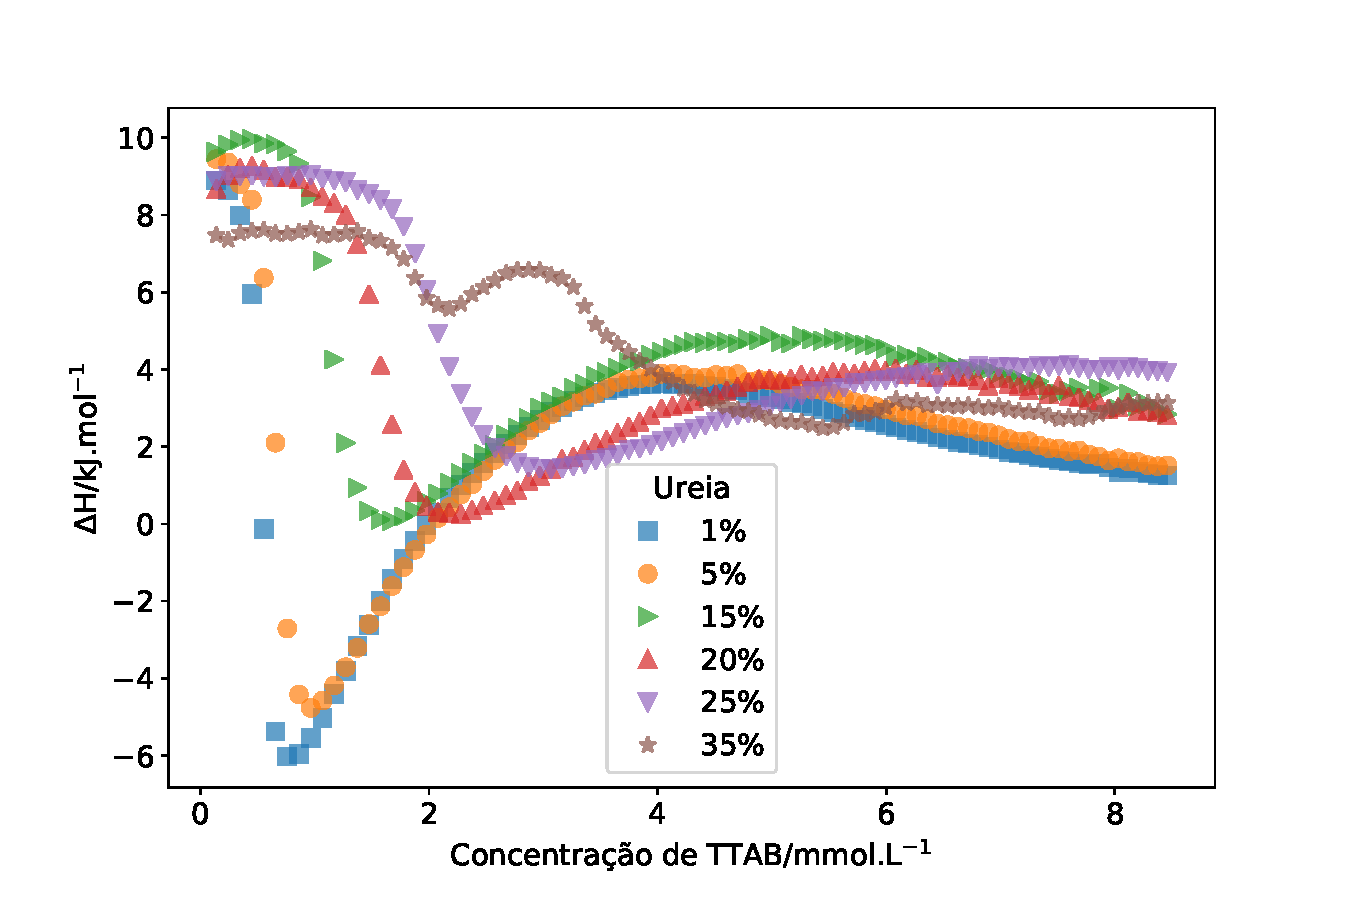
\includegraphics[width=0.7\textwidth]{imagens/itc/ITC_MG_ur}
				\caption{Efeito da concentração de ureia nas curvas de titulação de formação de micelas gigantes. A concentração de salicilato de sódio na cela de amostra é de 1,5\mM. A concentração do aditivo está em \% (m/m).}
				\label{fig:itc_mg_ureia}
			\end{figure}
		
			O comportamento da ureia seguiu o esperado, de acordo com a literatura, com um aumento de \cwlm{}. É interessante notar que o \DHwlm{} diminui com o aumento da concentração de ureia, o que sugere uma diminuição na adsorção de salicilato nas micelas. Em 35\% de ureia observa-se um perfil bastante diferente dos outros, porém nessa situação, ocorre a formação de um precipitado, cuja natureza será discutida na seção \ref{sec:cap_efeito_ureia}.
			
			Uma maneira de se resumir as curvas calorimétricas é através da concentração de formação de micelas gigantes (\cwlm) e a entalpia de micelização (\DHwlm). Dessa forma, podemos analisar o comportamento de todos os aditivos mais facilmente. A figura \ref{fig:cwlm_dhwlm_por_aditivo} resume isso, mostrando como essas propriedades variam com os aditivos, separadamente. A figura \ref{fig:cwlm_dhwlm_por_conc} mostra o mesmo, porém em função da concentração de aditivo.
			
			\begin{figure}[h]
				\begin{subfigure}[t]{0.5\textwidth}
					\centering
					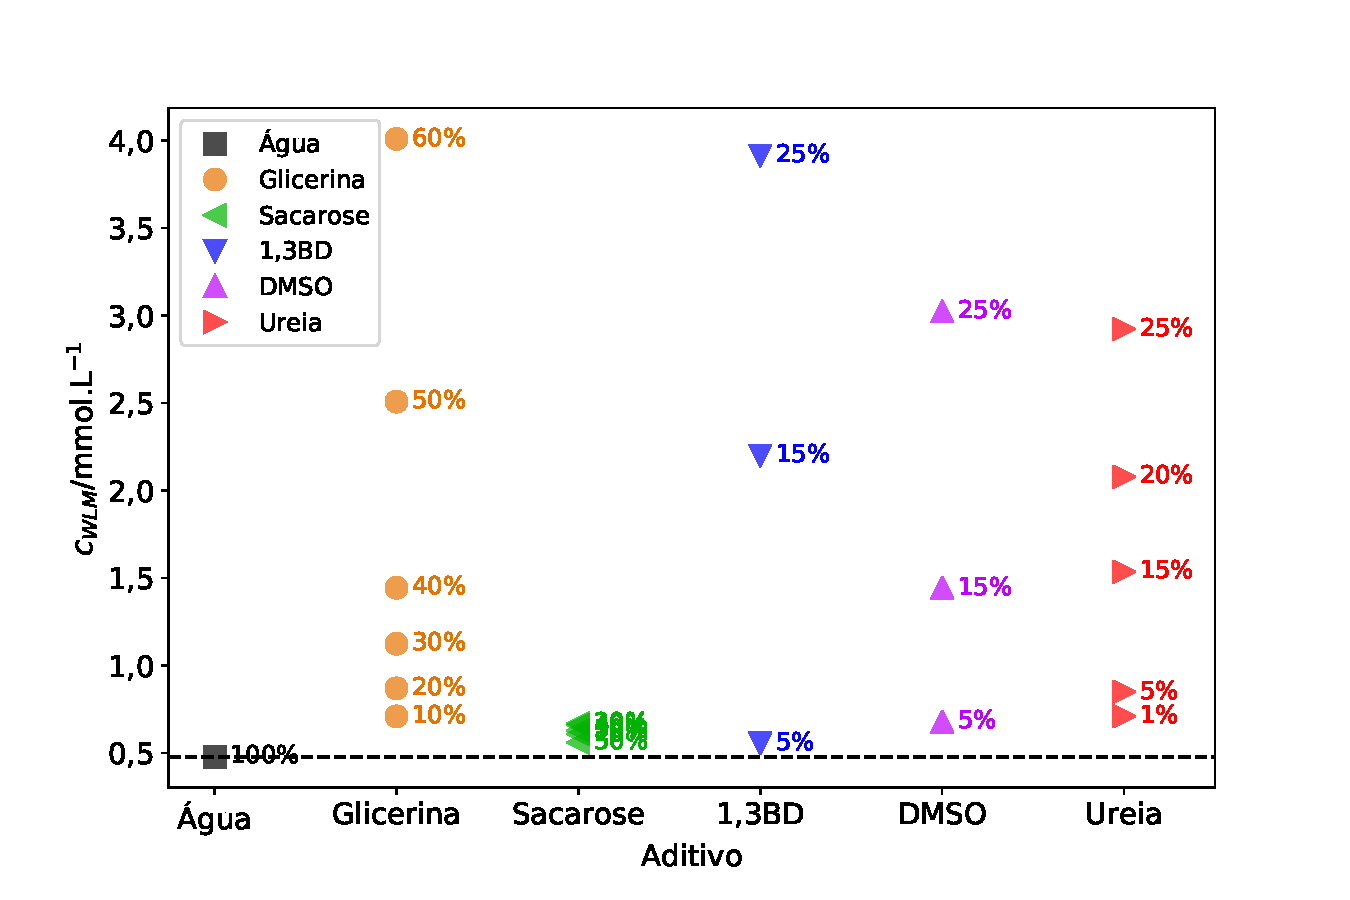
\includegraphics[width=\textwidth]{imagens/itc/Cwlm_por_Aditivo}
					\caption{\cwlm{}}
					\label{fig:cwlm_por_aditivo}
				\end{subfigure}%
				\begin{subfigure}[t]{0.5\textwidth}
					\centering
					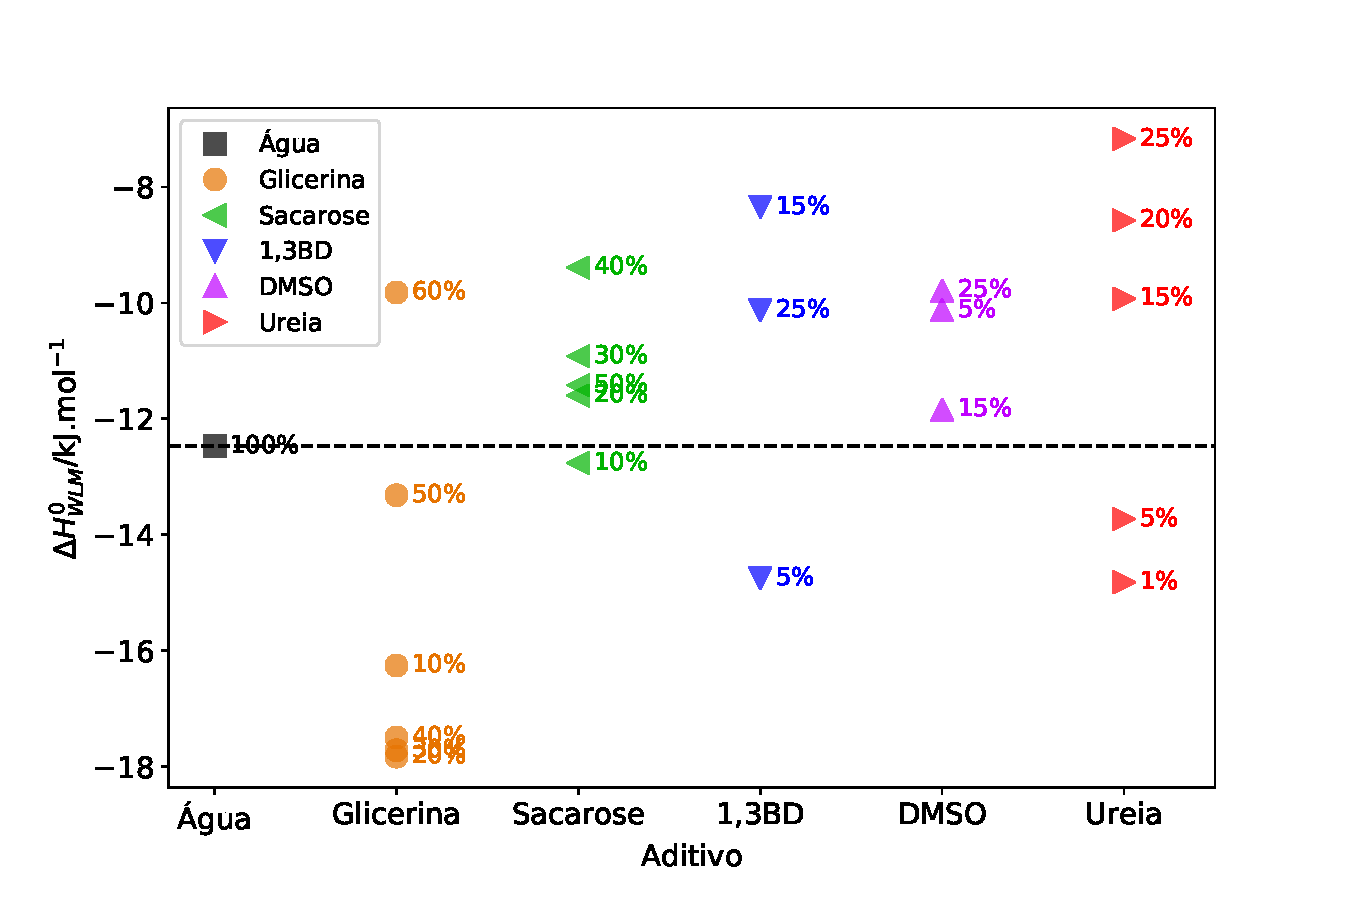
\includegraphics[width=\textwidth]{imagens/itc/DHwlm_por_Aditivo}
					\caption{\DHwlm{}}
					\label{fig:dhwlm_por_aditivo}
				\end{subfigure}
				\caption{\cwlm{} e \DHwlm{} em função dos aditivos e de sua concentração}
				\label{fig:cwlm_dhwlm_por_aditivo}
			\end{figure} 
		
			\begin{figure}[h]
				\begin{subfigure}[t]{0.5\textwidth}
					\centering
					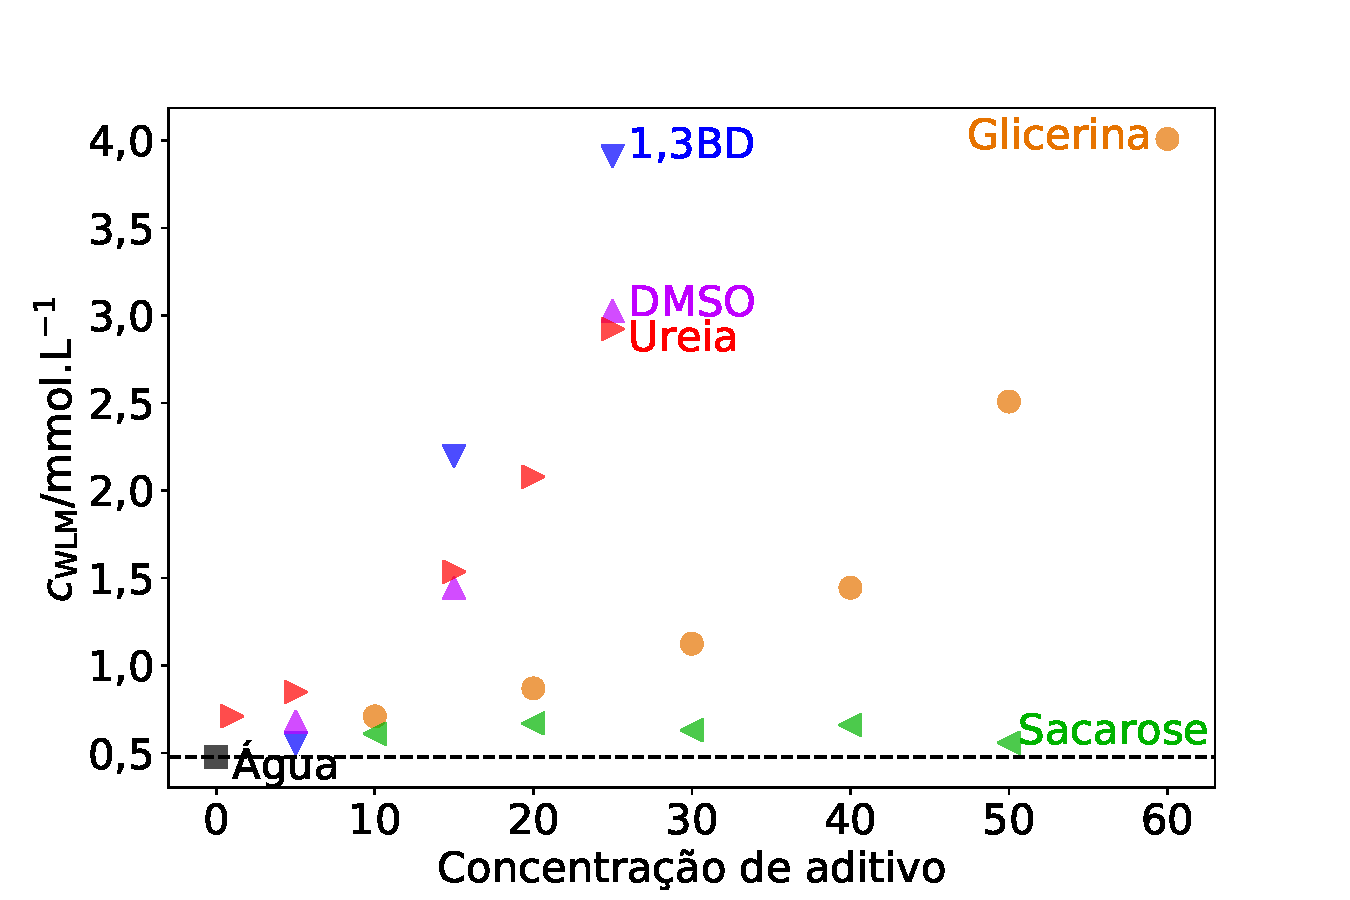
\includegraphics[width=\textwidth]{imagens/itc/Cwlm_por_conc}
					\caption{\cwlm}
					\label{fig:cwlm_por_conc}
				\end{subfigure} %
				\begin{subfigure}[t]{0.5\textwidth}
					\centering
					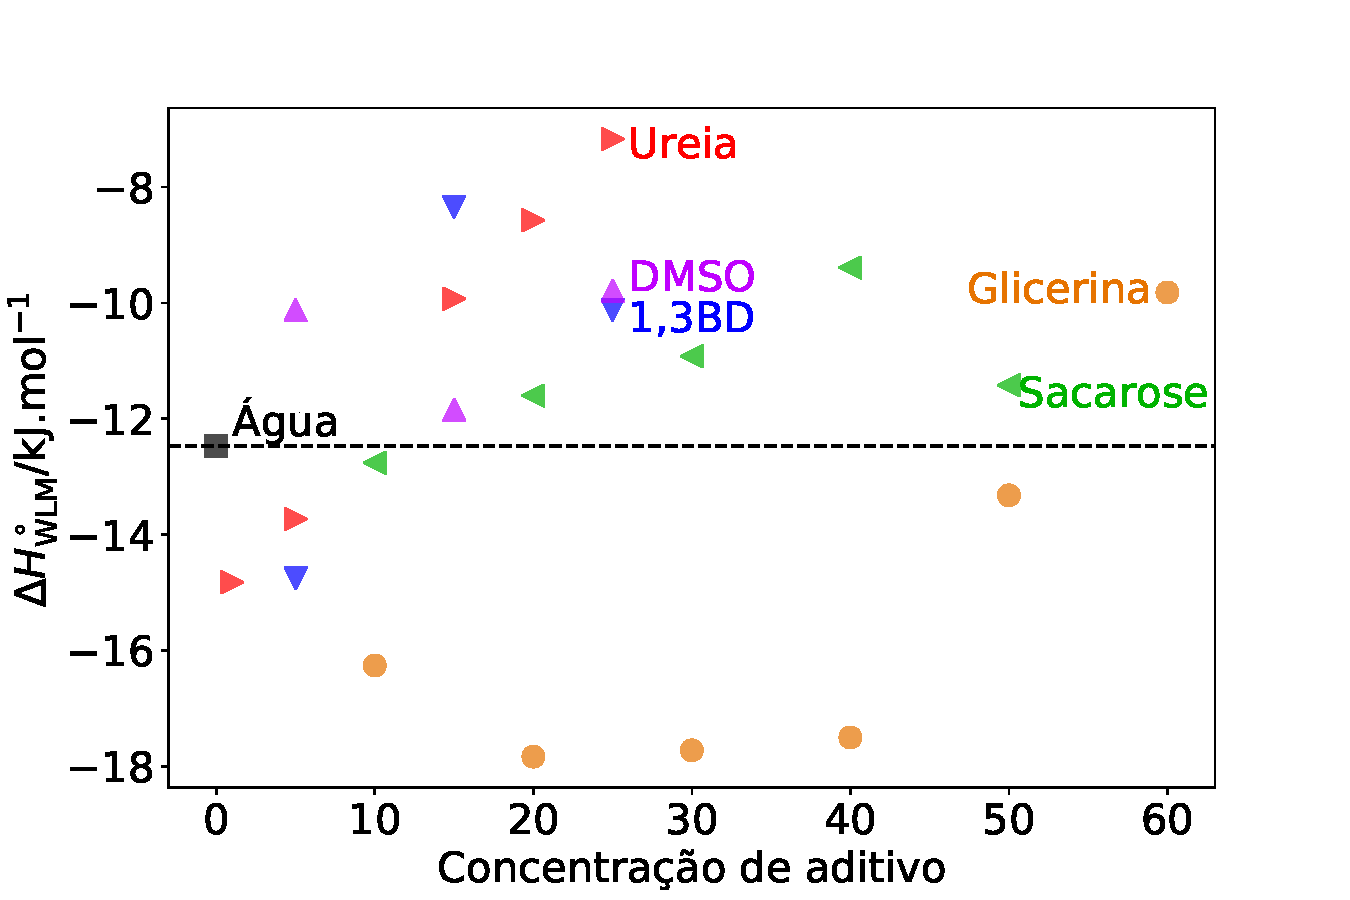
\includegraphics[width=\textwidth]{imagens/itc/DHwlm_por_conc}
					\caption{\DHwlm}
					\label{fig:dhwlm_por_conc}
				\end{subfigure}
				
				\caption{\cmc{} e \DHmic{} em função da concentração de aditivo.}
				\label{fig:cwlm_dhwlm_por_conc}
			\end{figure}
		
		\FloatBarrier
		
		\section{Efeito dos aditivos na calorimetria de micelização}
		
		A calorimetria de formação de micelas gigantes possui uma complexidade maior devido à presença do salicilato. Para facilitar a interpretação, foram obtidas informações da formação de micelas esféricas, titulando-se \TTAB{} em água. As figuras \ref{fig:itc_glicerina} -- \ref{fig:itc_ureia} mostram as curvas de titulação para glicerina, sacarose, 1,3-butanodiol, dimetilsulfóxido e ureia.
					
%			\begin{figure}[h]
%				\centering
%				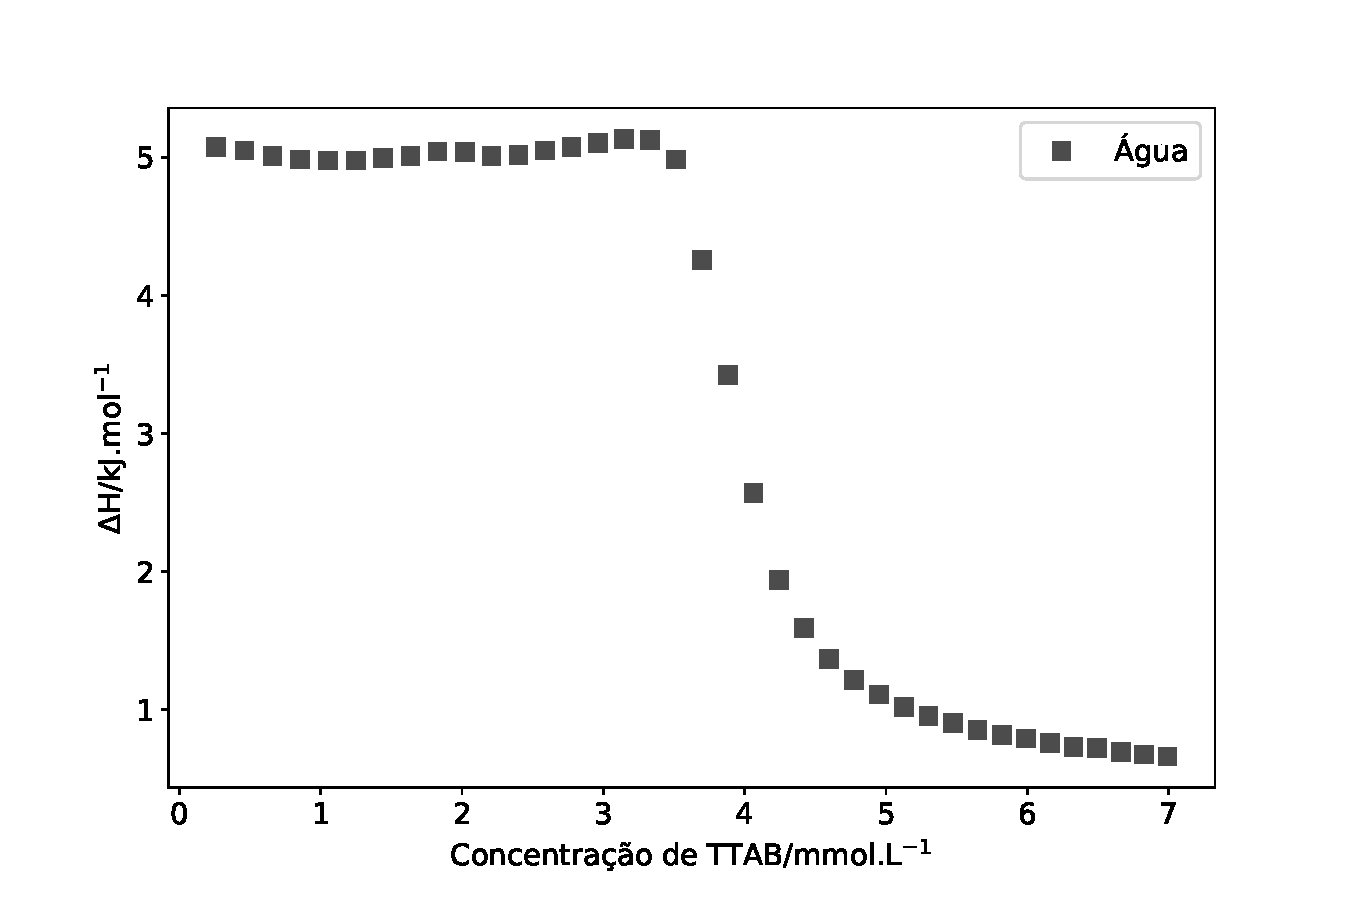
\includegraphics[width=0.7\textwidth]{imagens/itc/ITC_agua}
%				\caption{Titulação de \TTAB em água}
%				\label{fig:itc_agua}
%			\end{figure}
			
			\begin{figure}[h]
				\centering
				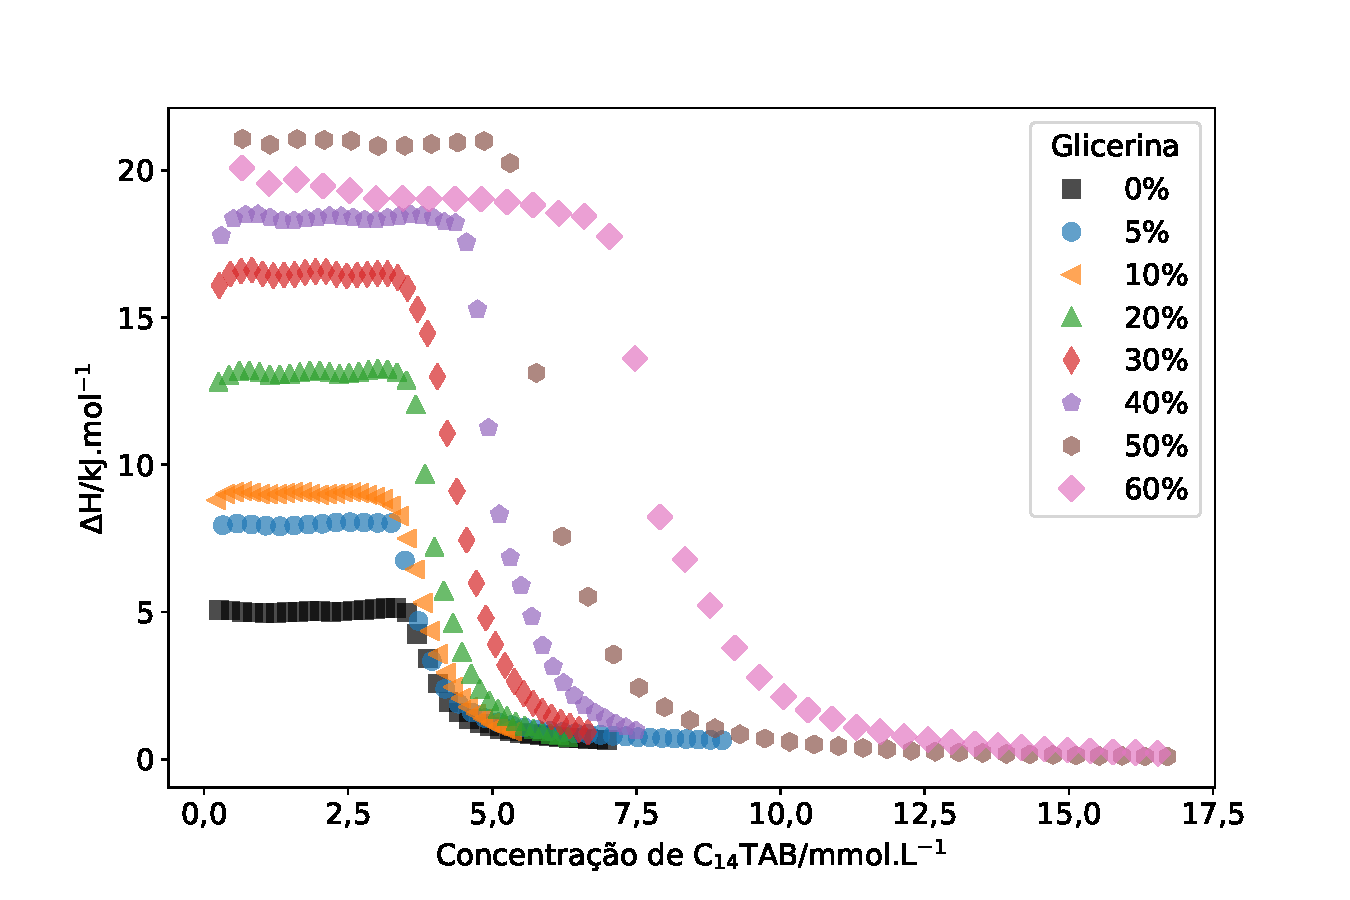
\includegraphics[width=0.7\textwidth]{imagens/itc/ITC_glic}
				\caption{Efeito da glicerina na titulação de \TTAB.}
				\label{fig:itc_glicerina}
			\end{figure}
		
			\begin{figure}[h]
				\centering
				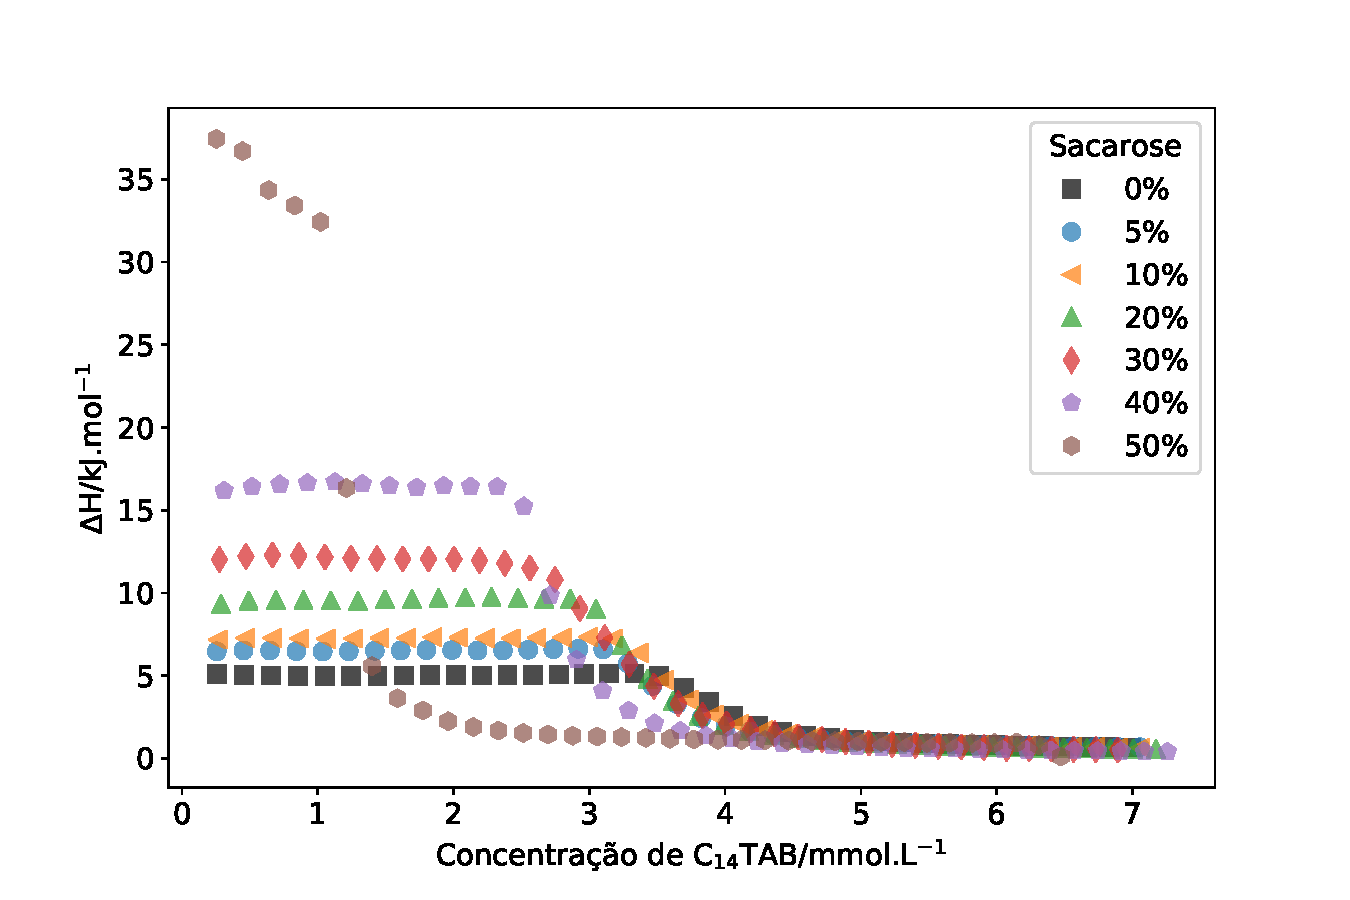
\includegraphics[width=0.7\textwidth]{imagens/itc/ITC_sac}
				\caption{Efeito de sacarose na titulação de \TTAB}
				\label{fig:itc_sacarose}
			\end{figure}
			
			O efeito da glicerina na formação de micelas é semelhante ao efeito em micelas gigantes, exceto pelo aumento do \DHmic{}. Mais interessante, porém, é que sacarose levou à uma diminuição da \cmc{}. Isso levanta duas perguntas. Em primeiro lugar, qual é o mecanismo de estabilização micelar, e depois, porque esse mecanismo não afeta a formação de micelas gigantes?
			
			% todo: ref
			A literatura aponta que os grupos hidroxila pode interagir com a superfície micelar, diminuindo a repulsão entre as cabeças, estabilizando as micelas. Porém, nas micelas gigantes, o grupo carboxilato do salicilato se encontra nessa mesma região, então há uma competição entre esses dois grupos. Como o carboxilato é carregado, interage mais fortemente com as micelas e impede que a sacarose exerça sua influência estabilizadora. 
			
			\begin{figure}[h]
				\centering
				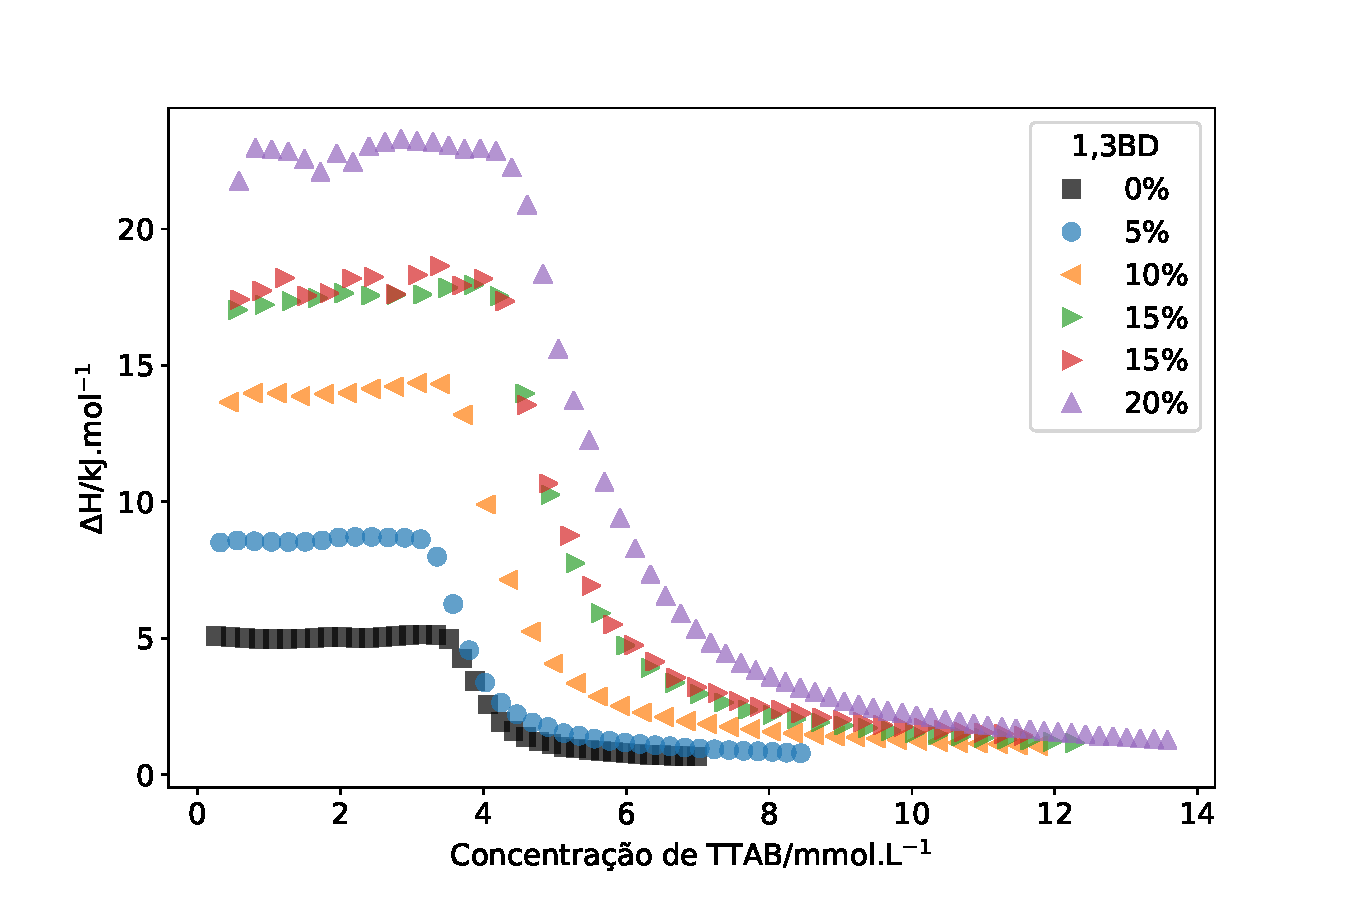
\includegraphics[width=0.7\textwidth]{imagens/itc/ITC_13BD}
				\caption{Efeito de 1,3-butanodiol na titulação de \TTAB}
				\label{fig:itc_13bd}
			\end{figure} 
		
			\begin{figure}[h]
				\centering
				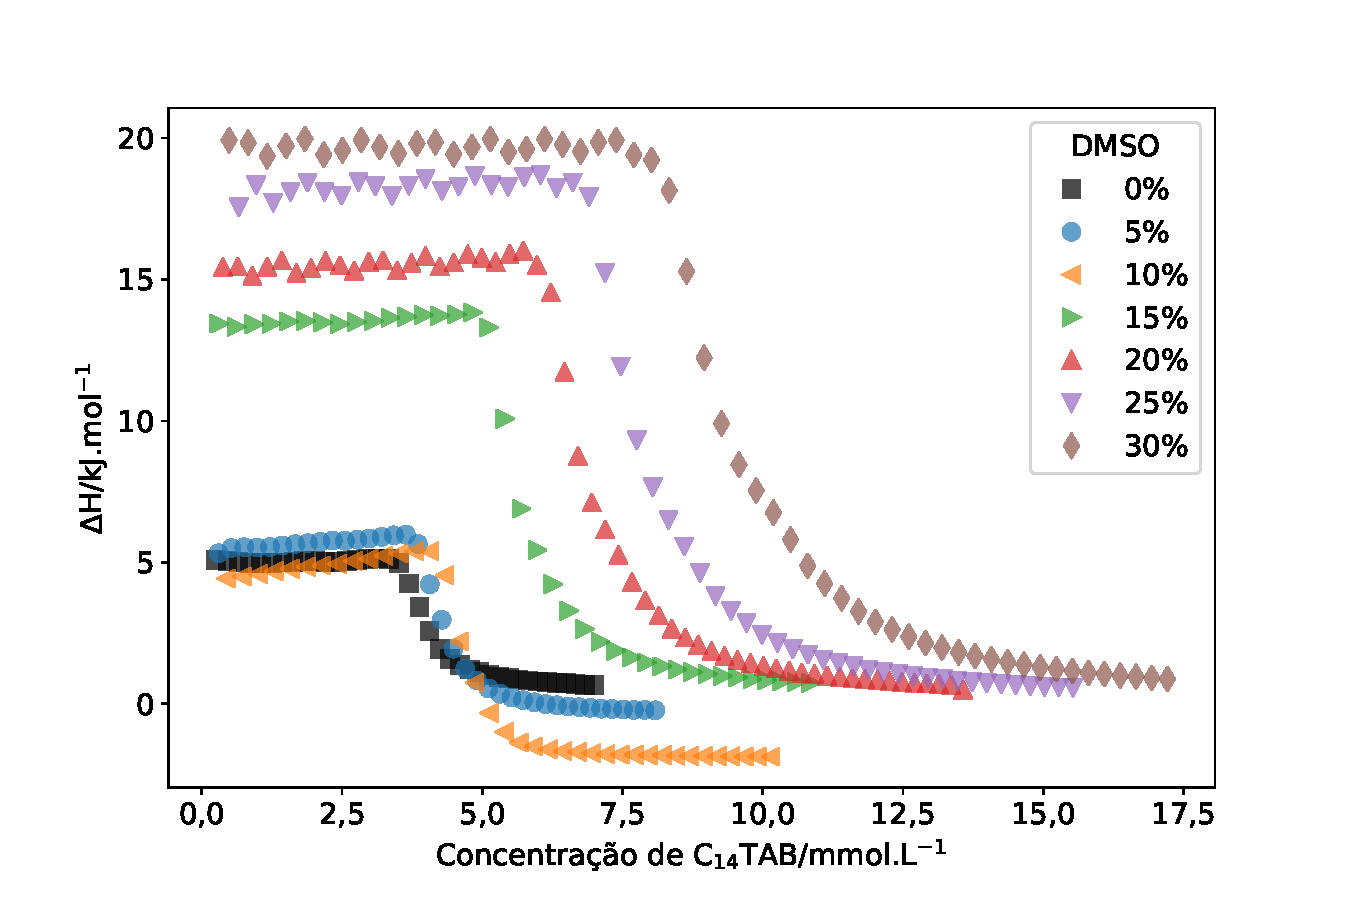
\includegraphics[width=0.7\textwidth]{imagens/itc/ITC_dmso}
				\caption{Efeito de dimetilsulfóxido na titulação de \TTAB.}
				\label{fig:itc_dmso}
			\end{figure}
			
			Novamente, o 1,3-BD e DMSO mostraram possuir comportamentos semelhantes entre si, portanto o mecanismo que influencia ambas as micelas gigantes quanto esféricas deve ser semelhante.
			
			\begin{figure}[h]
				\centering
				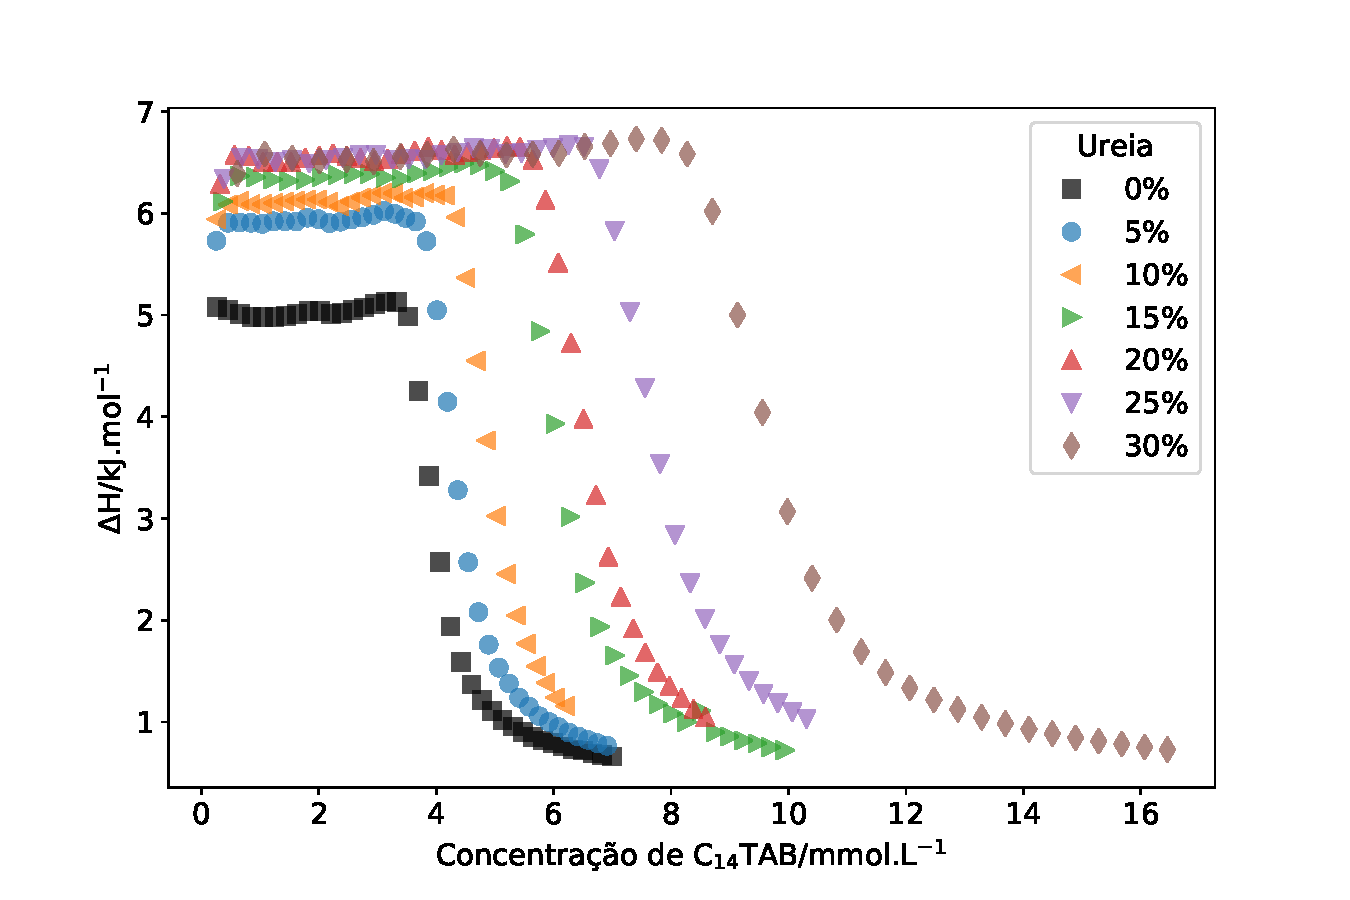
\includegraphics[width=0.7\textwidth]{imagens/itc/ITC_ur}
				\caption{Efeito de ureia na titulação de \TTAB.}
				\label{fig:itc_ureia}
			\end{figure}
		
		A ureia influencia aumentando a \cmc{}, como esperado, porém não afeta muito o \DHmic{}. Logo, como não há \Sal{} para ser dessorvido das micelas, devido à alta constante dielétrica do meio, não há variações de \DHmic.
		
		As concentrações micelares críticas (\cmc) e entalpias de micelização (\DHmic) foram utilizadas para resumir as informações desta seção. A figura \ref{fig:cmc_dh_por_composto} mostra como as propriedades são afetadas pelos vários aditivos e suas concentrações, separadamente, e a figura \ref{fig:cmc_dh_por_conc} faz o mesmo, porém em função da concentração de aditivo.
		
		\begin{figure}[h]
			\begin{subfigure}[t]{0.5\textwidth}
				\centering
				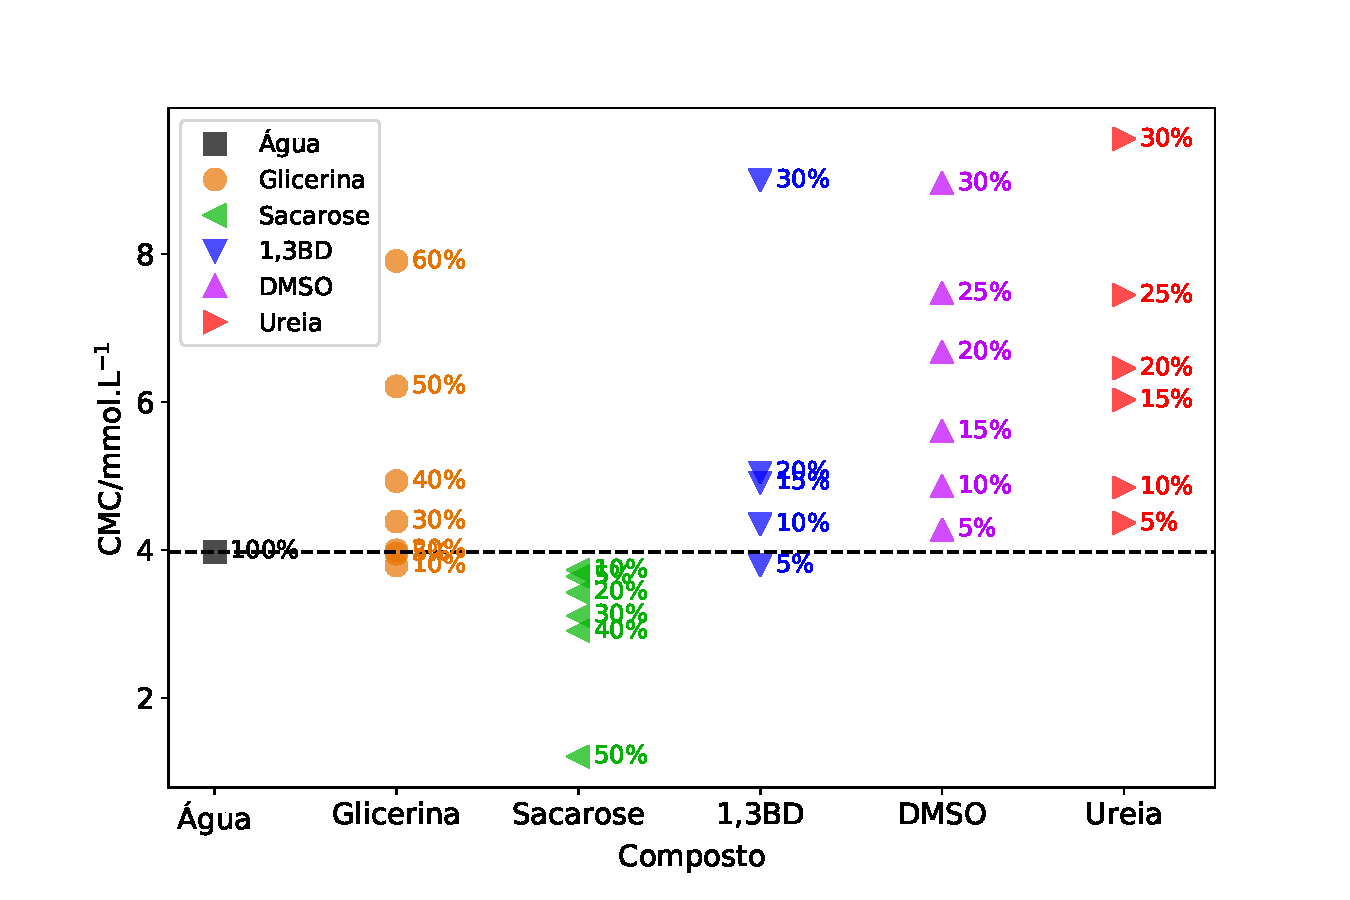
\includegraphics[width=\textwidth]{imagens/itc/CMC_por_composto}
				\caption{\cmc}
				\label{fig:cmc_por_composto}
			\end{subfigure} %
			\begin{subfigure}[t]{0.5\textwidth}
				\centering
				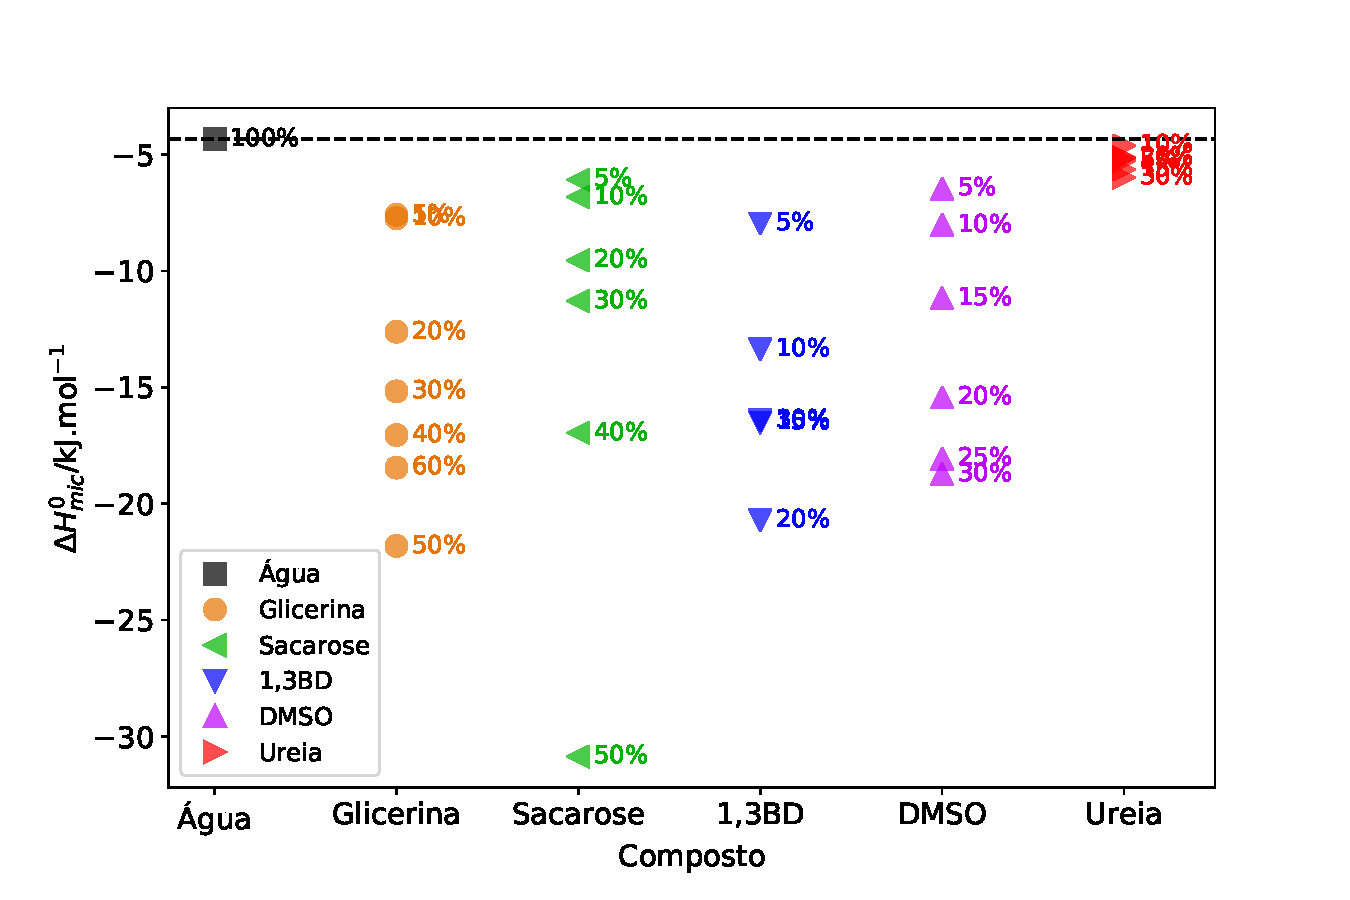
\includegraphics[width=\textwidth]{imagens/itc/DH_por_composto}
				\caption{\DHmic}
				\label{fig:dh_por_composto}
			\end{subfigure}
		
			\caption{\cmc{} e \DHmic{} para os vários aditivos}
			\label{fig:cmc_dh_por_composto}
		\end{figure}

		\begin{figure}[h]
			\begin{subfigure}[t]{0.5\textwidth}
				\centering
				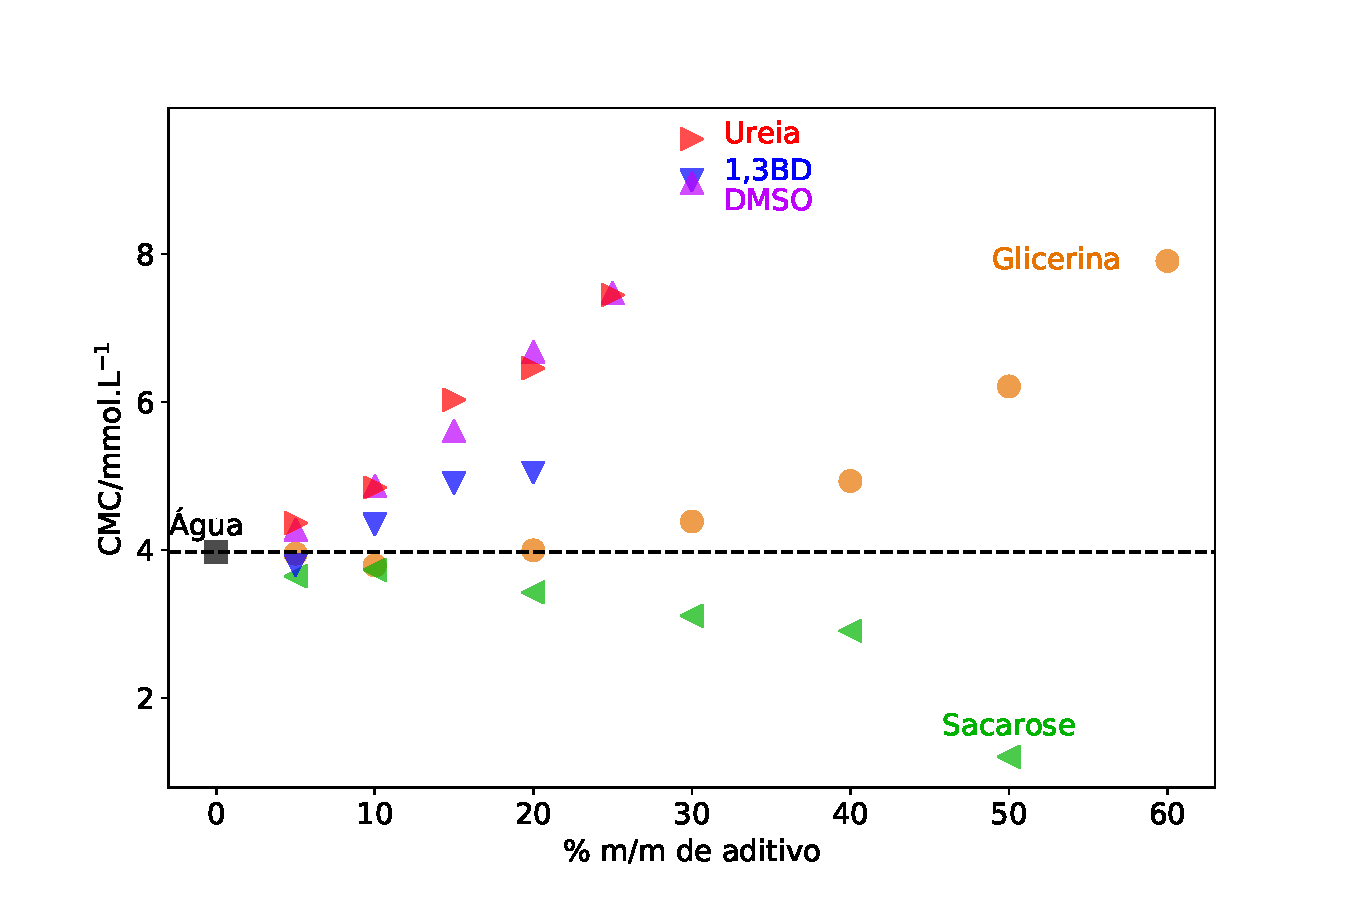
\includegraphics[width=\textwidth]{imagens/itc/ITC_cmc_adit}
				\caption{\cmc}
				\label{fig:cmc_por_conc}
			\end{subfigure} %
			\begin{subfigure}[t]{0.5\textwidth}
				\centering
				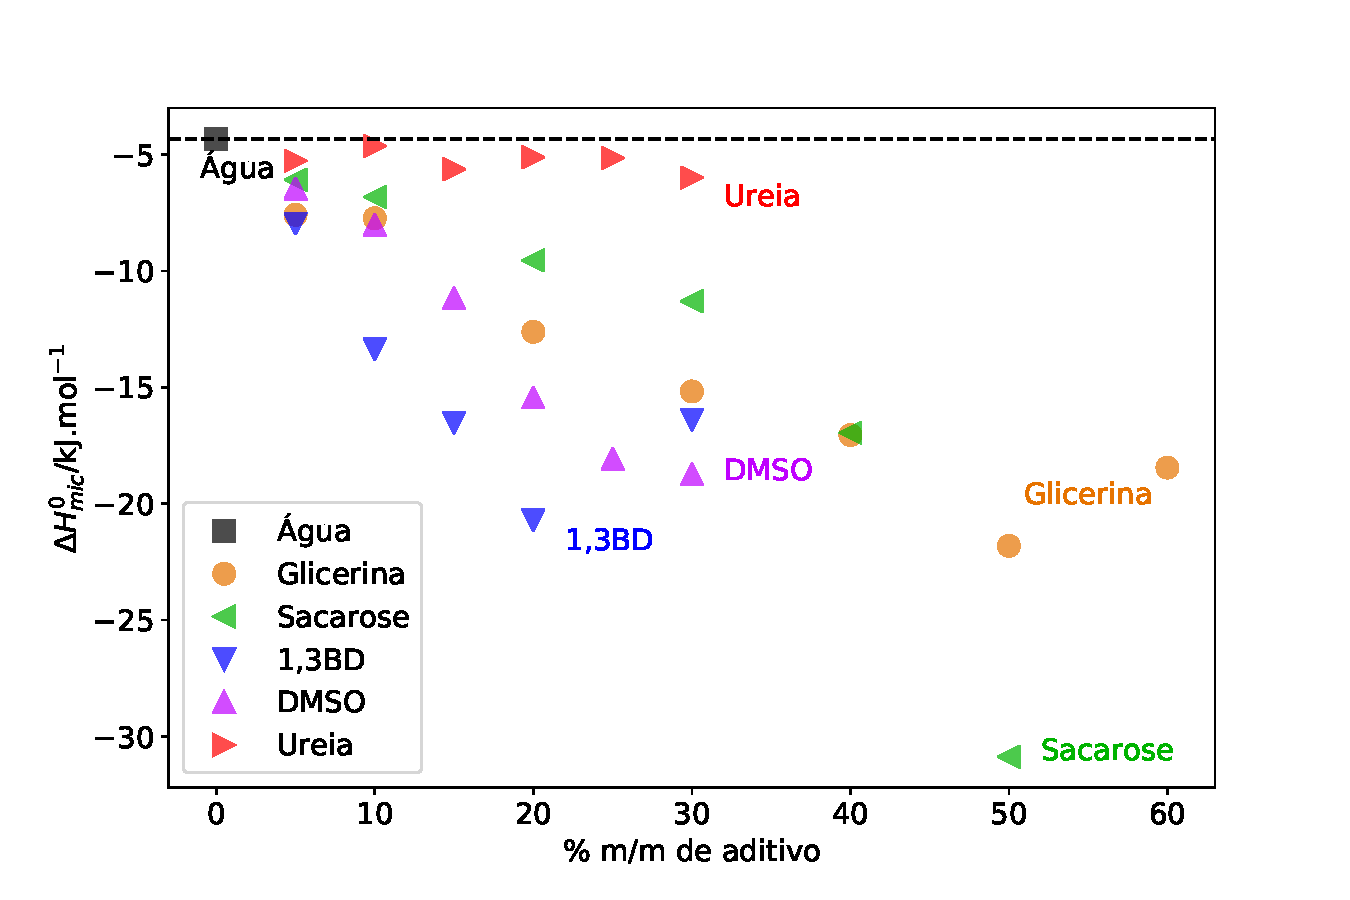
\includegraphics[width=\textwidth]{imagens/itc/ITC_DH_adit}
				\caption{\DHmic}
				\label{fig:dh_por_conc}
			\end{subfigure}
			
			\caption{\cmc{} e \DHmic{} em função da concentração de aditivo.}
			\label{fig:cmc_dh_por_conc}
		\end{figure}
	
		\FloatBarrier
		
	\chapter{Parâmetros estudados}
		
		Existem vários parâmetros físico-químicos que descrevem solventes. Inicialmente, o índice de refração foi escolhido com base nos estudos anteriores de Hoffmann. Esse parâmetro, definido como a relação da velocidade da luz no vácuo e no material em um determinado comprimento de onda (eq. \ref{eqn:def_n}) é relevante para a discussão pois está diretamente associado à polarizabilidade das moléculas através da equação de Lorenz-Lorentz, eq. \ref{eqn:lorenz_lorentz}.
		
		\begin{equation}
			n = \dfrac{c_0}{c}
			\label{eqn:def_n}
		\end{equation}
		
		\noindent onde \(n\) é o índice de refração, \(c_0\) é a velocidade da luz no vácuo e \(c\) é a velocidade da luz no meio.
		
		\begin{equation}
			\dfrac{n^2 - 1}{n^2 + 2}\dfrac{1}{\rho} = \dfrac{4\pi N_A}{3} \alpha_e^0
			\label{eqn:lorenz_lorentz}  % todo: ref olson1975
		\end{equation}
		
		\noindent onde \(n\) é o índice de refração, \(\rho\) é a densidade molar, \(N_A\) é o número de Avogadro e \(\alpha_e^0\) é a polarizabilidade eletrônica molecular isolada.
		
		É possível transformar essa equação para encontrar a polarização molar \(P_m\)

		\begin{equation}
			P_m = \dfrac{n^2 - 1}{n^2 + 1} \cdot \dfrac{M_r}{\rho}
		\end{equation}
		
		\noindent onde \(M_r\) é a massa molar relativa e \(\rho\) é a densidade do solvente.
		
		Quanto maior for a polarizabilidade, mais fortes são as interações dispersivas entre duas moléculas, como mostra a equação \ref{eqn:U_dispersiva}.
		
		\begin{equation}
			U_{\textrm{dispersiva}} = - \dfrac{1}{(4 \pi \varepsilon_0)^2} \dfrac{3 \alpha_1 \alpha_2}{2 r^6} \left( \dfrac{I_1 \cdot I_2}{I_1 + I_2} \right)
			\label{eqn:U_dispersiva}
		\end{equation}  % todo: achar ref [33], cap2 do livro de solvente em reações orgânicas, 
		
		\noindent onde \(\varepsilon_0\) é a constante dielétrica do vácuo, \(\alpha_1\) e \(\alpha_2\) são as polarizabilidades de duas moléculas, \(r\) é a distância entre as moléculas e \(I_1\) e \(I_2\) são os potenciais de ionização das duas moléculas. Controlando-se a polarizabilidade das espécies é possível ajustar a atração dispersiva entre elas.
		
		Na área coloidal, é necessário somar todas as contribuições atrativas e repulsivas de todas as moléculas que compõem o coloide para se obter a atração ou repulsão coloidal. Isso se traduz na constante de Hamaker, que modula essas atrações (eq. \ref{eqn:Hamaker}). Essas atrações ocorrem através de um solvente, então é necessário considerá-lo no cálculo das atrações intercoloidais.
		
		\begin{equation}
		H = \dfrac{3}{4}kT \left[  \dfrac{\varepsilon_a - \varepsilon_s}{\varepsilon_a + \varepsilon_s}  \right]^2 + %
		    \dfrac{3}{16\sqrt{2}} h\nu \dfrac{ \left(  n_a^2 - n_s^2  \right)^2}{\left(  n_a^2 + n_s^2  \right)^{3/2}}
		\label{eqn:hamaker}
		\end{equation}
		
		\noindent onde $\varepsilon_a$ e $\varepsilon_s$ são as constantes dielétricas dos agregados e do solvente na frequência zero, respectivamente, $h$ é a constante de Planck e $\nu$ é a frequência da absorção dominante no UV (tipicamente $3 \times 10^{15} s^{-1}$) [XYZ]. O primeiro termo da expressão é pequeno, perto de $kT$, logo quando $n_s \rightarrow n_a$, $H \rightarrow 0$, a atração intermicelar se torna muito fraca.
		% \cite{Israelachvili2011}
	
		A constante dielétrica \(\varepsilon\) é um parâmetro relacionado à polaridade do solvente. Quanto maior for a constante dielétrica, mais fácil é a separação de cargas no solvente pois menor é sua atração (\ref{eqn:U_eletrostatica}). A constante dielétrica (também chamada de permissividade) é medida colocando-se o material entre duas placas carregadas de um capacitor. O campo elétrico resultante \(E\) é menor do que o campo elétrico no vácuo, \(E_0\), e a razão \(\sfrac{E_0}{E}\) fornece a constante dielétrica do meio. Devido ao campo elétrico, as moléculas alinham seus dipolos, e caso o solvente não possua dipolos permanentes, serão criados dipolos induzidos devido ao campo, causando a polarização. Quanto maior for a polarização, maior é a queda, e maior é a constante dielétrica. Caso existam interações cooperativas solvente/solvente, como a associação em cadeias por ligações de hidrogênio intramoleculares, é possível obter valores de constante dielétrica muito altas, como 180 para amidas secundárias. Isso foi observado para a ureia, neste trabalho.
		
		\begin{equation}
			U_{\textrm{eletrostática}} = \dfrac{1}{4 \pi \varepsilon_r} \dfrac{q_1 q_2}{r^2}
			\label{eqn:U_eletrostatica}  % ref: Atkins Físico-Química
		\end{equation}
		
		\noindent onde \(\varepsilon_r\) é a constante dielétrica relativa entre o meio e o vácuo, \(\varepsilon_r = \sfrac{\varepsilon}{\varepsilon_0}\).
		
		Interessantemente, a constante dielétrica também está relacionada à polarizabilidade molecular, através da equação de Clausius-Mossotti \ref{eqn:clausius_mossotti}, que não considera a contribuição do momento de dipolo permanente.
		
		\begin{equation}
			\dfrac{\varepsilon_r - 1}{\varepsilon_r + 2} = \dfrac{\rho N_A \alpha}{3 M \varepsilon_0}
			\label{eqn:clausius_mossotti}
		\end{equation}
		
		Outro parâmetro relacionado à polaridade do solvente é o momento de dipolo, \(\mu\). É possível combinar ambos a constante dielétrica e o momento de dipolo no fator eletrostático, \emph{IT}, mas esses parâmetros não foram considerados neste trabalho pois os solventes são primariamente aquosos. % Ref [101] do capítulo 3
		
		Dois parâmetros podem ser utilizados para descrever a estruturação de um solvente, a densidade de energia coesiva \(c\) (eq. \ref{eqn:densidade_energia_coesiva}), e a pressão interna \(\pi\) (eq. \ref{eqn:pressao_interna}).  % refs [98-100, 175] do cap 3 do livro de propriedades de solvente
		
		\begin{equation}
			c = \dfrac{\Delta U_V}{V_m} = \dfrac{\Delta H_V - R\cdot T}{V_m}
			\label{eqn:densidade_energia_coesiva}
		\end{equation}
		
		\begin{equation}
			\pi = \left( \dfrac{\partial U}{\partial V_m} \right)_T
			\label{eqn:pressao_interna}
		\end{equation}
		
		\noindent onde \(\Delta U_V\) e \(\Delta H_V\) são a energia interna e entalpia de vaporização e \(V_m\) é o volume molar do líquido. A razão de se utilizar a entalpia/energia interna de vaporização é a seguinte. Ao levar um líquido de seu estado condensado para o estado gasoso, todas as ligações líquido-líquido tiveram que ser rompidas. Logo, dividindo-se essa energia pelo volume molar obtemos uma densidade de energia coesiva.
		
		A pressão interna, por sua vez, é a energia necessária para abrir uma cavidade no solvente, pois a variação de volume é necessariamente pequena, de modo a acomodar o soluto. Esse parâmetro é resultado das forças atrativas serem mais fortes que as repulsivas, e portanto está mais relacionado às interações dispersivas e dipolo-dipolo. Já \(c\) está relacionado à interações solvente-solvente específicas, como a ligação de hidrogênio.
		
		A diferença entre esses dois parâmetros (\(c - \pi\)) fornece uma medida da força das ligações de hidrogênio, e a razão \(n = \sfrac{\pi}{c}\) fornece uma medida da relação entre a força das ligações de hidrogênio e outras atrações. Essa razão se aproxima de 1 para hidrocarbonetos e é próxima de zero para solventes com fortes ligações de hidrogênio. O quadrado de \(c\) é conhecido também como o parâmetro de solubilidade de Hildebrand, \(\delta\).
		
		Porém, os solventes utilizados neste trabalho são todos compostos principalmente por água, e em alguns casos os aditivos são sólidos (ureia, sacarose). Além disso, obter esses parâmetros para as misturas não é uma tarefa para qual o laboratório está equipado. Portanto, é necessário utilizar outro parâmetro que esteja relacionado à estruturação do solvente.
		
		Um parâmetro que pode ser utilizado é o parâmetro de Gordon, definido na equação \ref{eqn:Gordon}, que é baseado na tensão superficial, equação \ref{eqn:tens_superficial}.

		\begin{equation}
			G = \dfrac{\gamma}{\bar{V}_m^{\frac{1}{3}}}
			\label{eqn:Gordon}
		\end{equation}
		
		\begin{equation}
			\bar{V}_m = \bar{V}_{m_{1}}x_1 + \bar{V}_{m_{2}}x_2
			\label{eqn:volume_molar_médio}
		\end{equation}
		
		\noindent onde \(\gamma\) é a tensão superficial do líquido e \(\bar{V}_m\) é o volume molar do líquido que, quando houver mais de um, pode-se utilizar a equação \ref{eqn:volume_molar_médio} para calculá-lo.
		
		\begin{equation}
		\gamma = \left( \dfrac{\partial G}{\partial A}  \right)_{T,P,n}
		\label{eqn:tens_superficial}
		\end{equation}
		
		\noindent onde, neste caso \(G\) se refere à energia livre de Gibbs e \(A\) a área de superfície.
		
		A razão de se utilizar o parâmetro de Gordon vem de um argumento semelhante ao parâmetro de densidade de energia coesiva. Neste caso, o aumento da área superficial de um líquido necessita da quebra de interações líquido-líquido das moléculas que vão para a superfície. Um líquido com interações intermoleculares fracas possui uma tensão superficial baixa, pois é fácil quebrar essas ligações. Por outro lado, um líquido com interações intermoleculares fortes, como a água, possui uma tensão superficial bastante alta. Uma grande vantagem de se utilizar o parâmetro de Gordon é que as medidas de tensão superficial de misturas são facilmente realizadas, necessitando então somente a conversão de \(\gamma\) para \(G\). Porém, [XYZ] nota que \(c\) é um parâmetro melhor para descrever a energia coesiva % todo: referenciar o livro Christian Reichardt
	
%		Devido à essa relação, é possível correlacionar o índice de refração à constante dielétrica, obtendo a eq. \ref{eqn:n_epsilon}
%		
%		\begin{equation}
%			n = \varepsilon_r^{1/2}
%			\label{eqn:n_epsilon}
%		\end{equation}  % todo: pensar sobre essa equação e se ela realmente vale para as coisas aqui. Não parece ser tão assim
		
		\section{Índice de refração}
		
		A figura \ref{fig:indice_refracao} mostrou como o índice de refração varia com a concentração de aditivo. Como os resultados reológicos evidenciaram, considerar somente o índice de refração não é uma maneira muito boa para explicar o comportamento reológico.
		
		Caso contrário, haveria um padrão notável num gráfico comparativo das concentrações e entalpias. Isso está evidenciado nas figuras \ref{fig:cmc_dh_por_n} e \ref{fig:cwlm_dhwlm_por_n}, onde não há um padrão geral observado para todos os aditivos.
		
		\begin{figure}[h]
			\begin{subfigure}[t]{0.5\textwidth}
				\centering
				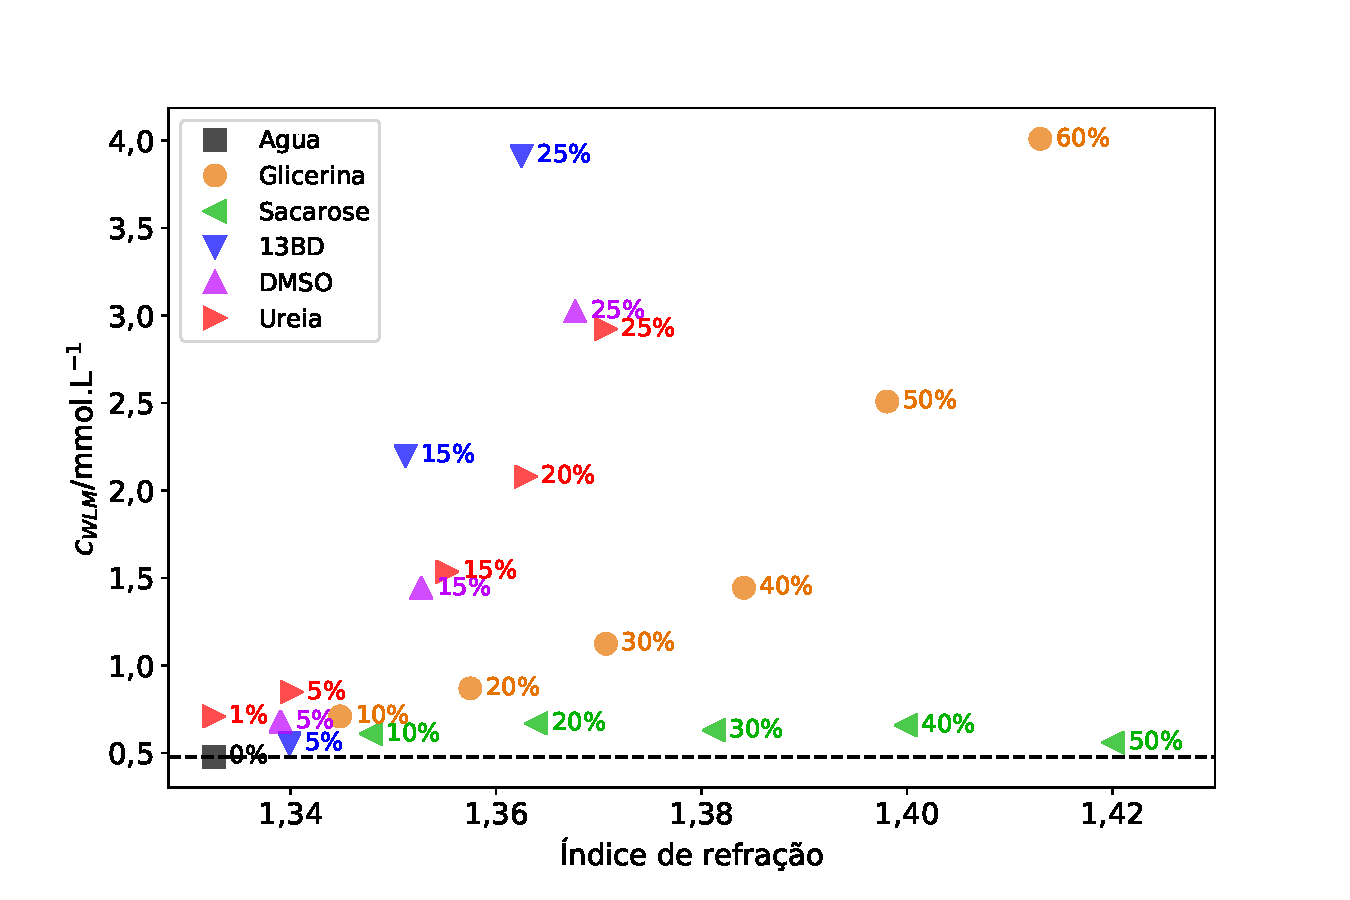
\includegraphics[width=\textwidth]{imagens/itc/Cwlm_por_n}
				\caption{\cwlm}
				\label{fig:cwlm_por_n}
			\end{subfigure} %
			\begin{subfigure}[t]{0.5\textwidth}
				\centering
				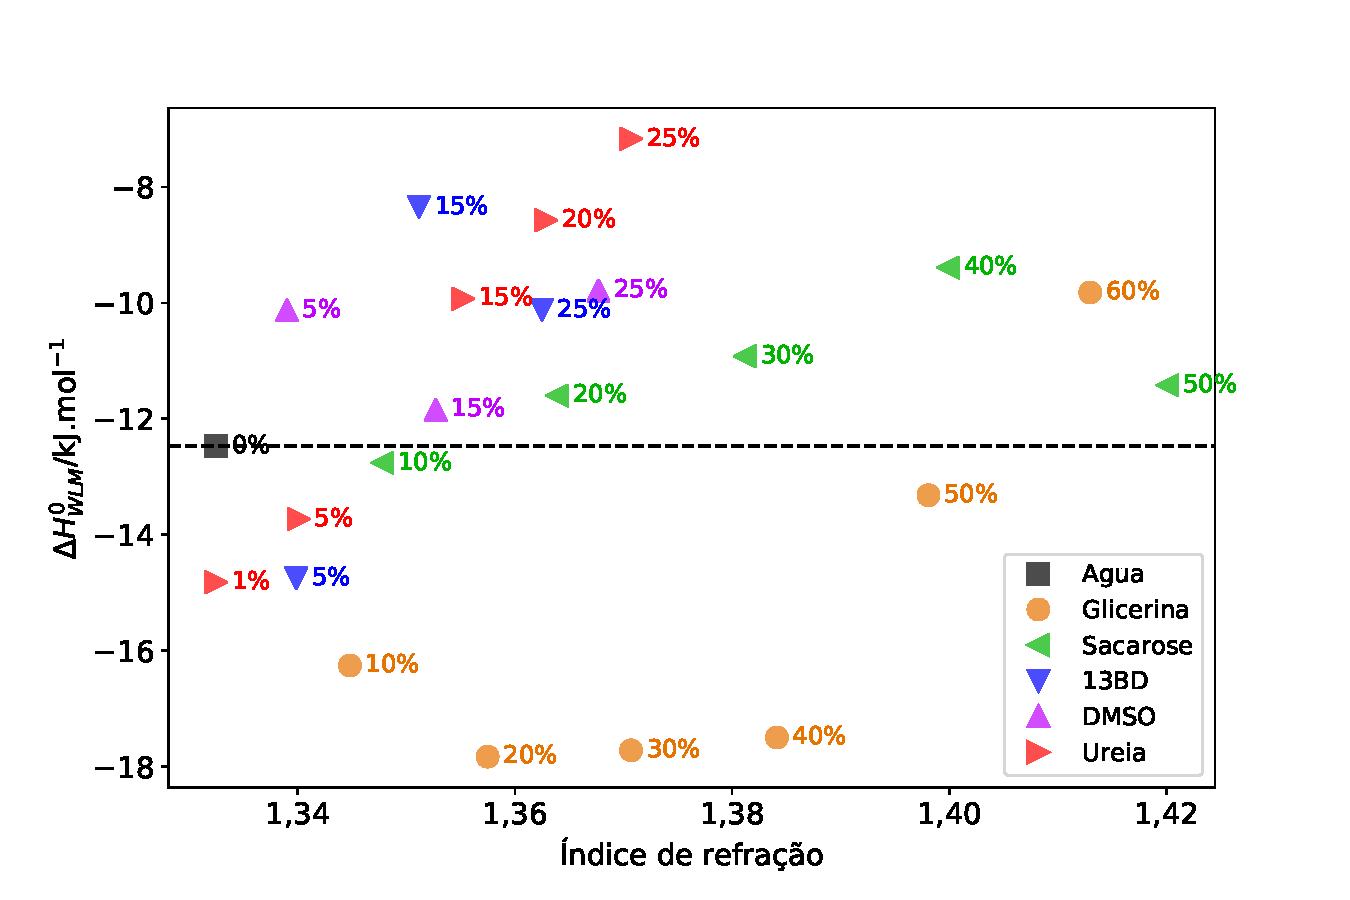
\includegraphics[width=\textwidth]{imagens/itc/DHwlm_por_n}
				\caption{\DHwlm}
				\label{fig:dhwlm_por_n}
			\end{subfigure}
			
			\caption{\cwlm{} e \DHwlm{} em função do índice de refração.}
			\label{fig:cwlm_dhwlm_por_n}
		\end{figure}
		
		\begin{figure}[h]
			\begin{subfigure}[t]{0.5\textwidth}
				\centering
				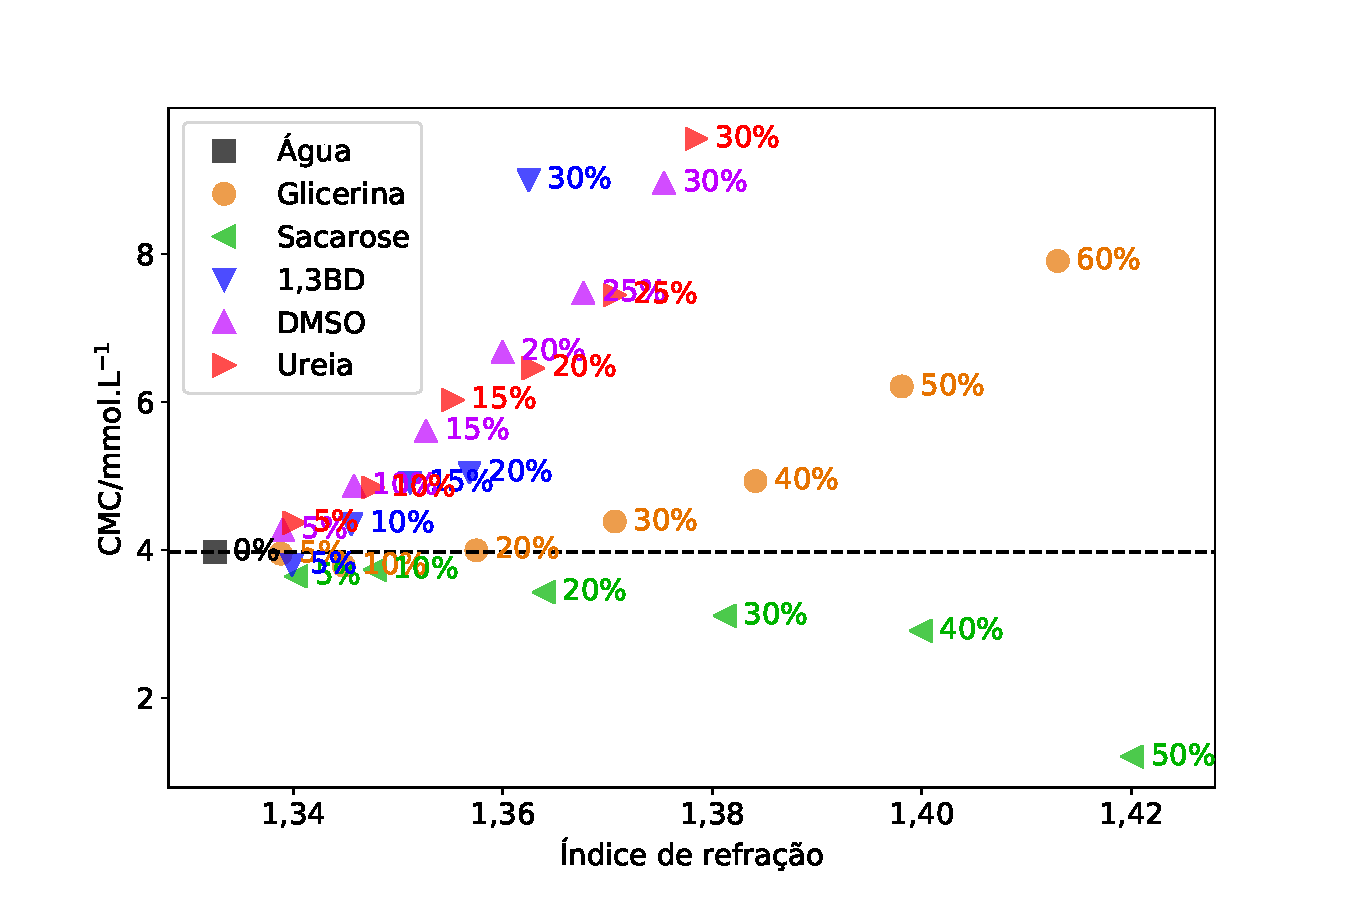
\includegraphics[width=\textwidth]{imagens/itc/CMC_por_n}
				\caption{\cmc}
				\label{fig:cmc_por_n}
			\end{subfigure} %
			\begin{subfigure}[t]{0.5\textwidth}
				\centering
				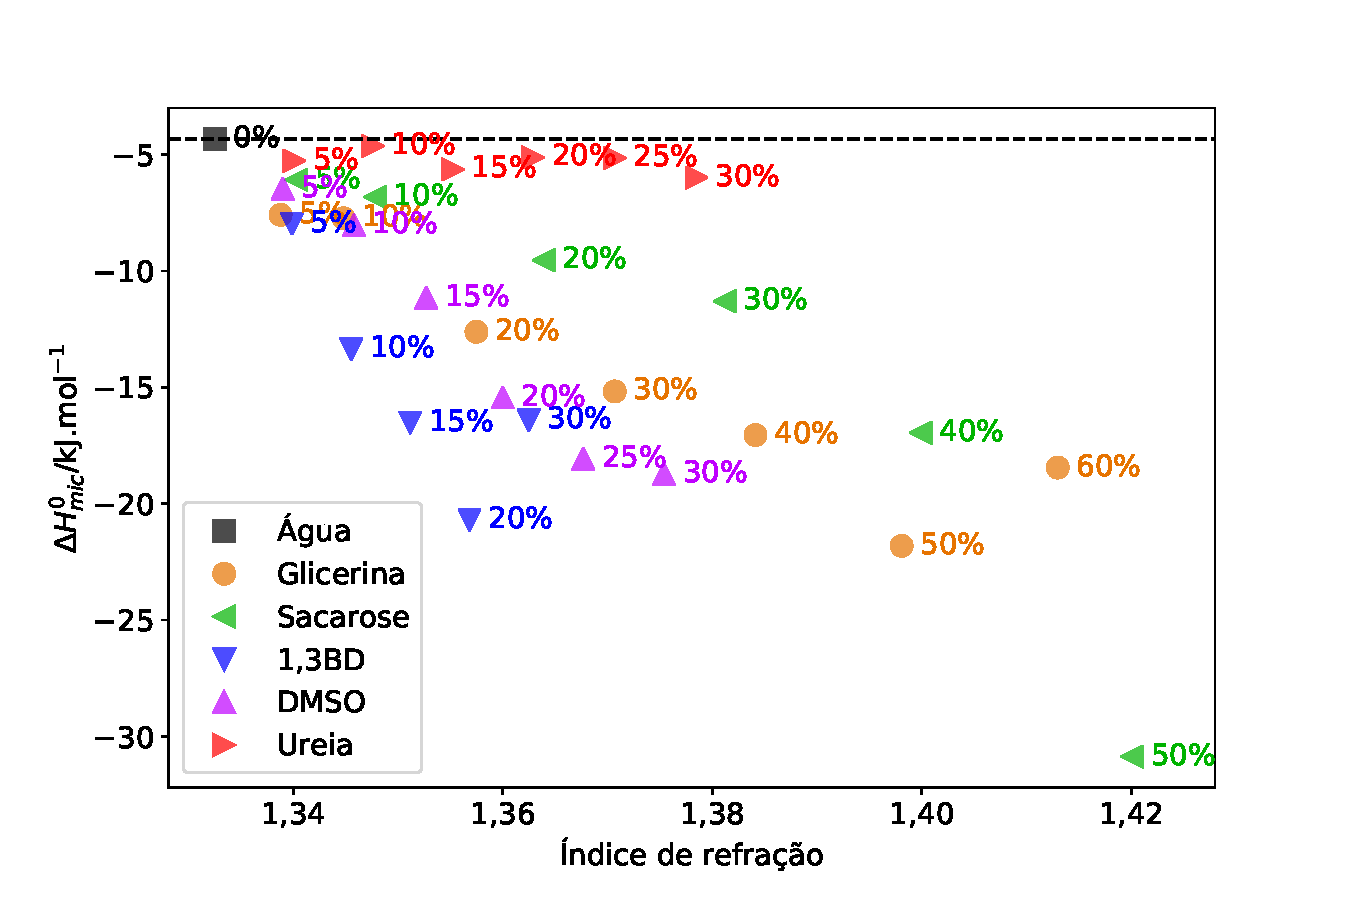
\includegraphics[width=\textwidth]{imagens/itc/DH_por_n}
				\caption{\DHmic}
				\label{fig:dh_por_n}
			\end{subfigure}
			
			\caption{\cmc{} e \DHmic{} em função do índice de refração.}
			\label{fig:cmc_dh_por_n}
		\end{figure}

		Comparando-se as figuras \ref{fig:cwlm_dhwlm_por_n} e \ref{fig:cmc_dh_por_n}, pode-se observar que há uma correlação entre a formação de micelas gigantes e as concentrações críticas. Aparentemente há um grupo composto de 1,3BD, DMSO e ureia. Glicerina e sacarose se comportam bastante diferentemente, sendo que sacarose possui o comportamento mais diferenciado, não havendo mudança na \cwlm{} e uma diminuição da \cmc{}.
		
		Agrupamentos desse tipo não podem ser feitos com as entalpias, que parecem ter valores bastante variáveis. Porém, é necessário enfatizar que os valores de entalpia obtidos para a formação de micelas gigantes não são tão confiáveis quanto os de formação de micelas esféricas. Para obter os perfis completos de formação de micelas gigantes, foi necessário aumentar a concentração de surfactante na seringa. Isso reduz a precisão na região inicial do perfil, onde é calculado o \DHwlm. Além disso, a resolução dos entalpogramas obtidos pelo calorímetro PEAQ é menor (39 pontos) do que no VP-ITC (90 pontos). Esse problema possui menor relevância para \cwlm{}, que foi definida como sendo o ponto mínimo da curva, não uma subtração de duas regiões pré e pós-micelar.  Apesar disso, o padrão observado para as mudanças de entalpia na presença de ureia podem ser explicadas pelo aumento da constante dielétrica do meio, como previamente mencionado.
	
		É interessante notar que as figuras que comparam as concentrações de formação e entalpias com o índice de refração (Figs. \ref{fig:cwlm_dhwlm_por_n} e \ref{fig:cwlm_dhwlm_por_conc}, \ref{fig:cmc_dh_por_n} e \ref{fig:cmc_dh_por_conc}) e a concentração de aditivo são bastante semelhantes. Isso se deve à dependência praticamente linear em baixas concentrações do índice de refração com a concentração de aditivo na escala mássica, um dos motivos para essa escalar ser escolhida.
		
		\FloatBarrier
		
		\section{Constante dielétrica}
		
		A constante dielétrica está relacionada ao grau de dissociação de espécies iônicas em solução. Quanto maior a constante, maior o grau de dissociação. Isso resulta, por exemplo, no aumento da \cmc{} pois há menos contraíons para reduzir a carga superficial micelar. A contribuição desse parâmetro já havia sido levantada em um estudo anterior. % todo: ref.
		A figura \ref{fig:cte_dieletrica} mostra como a constante dielétrica varia em função da concentração de aditivo. %todo: refs

		
		\begin{figure}[h]
			\centering
			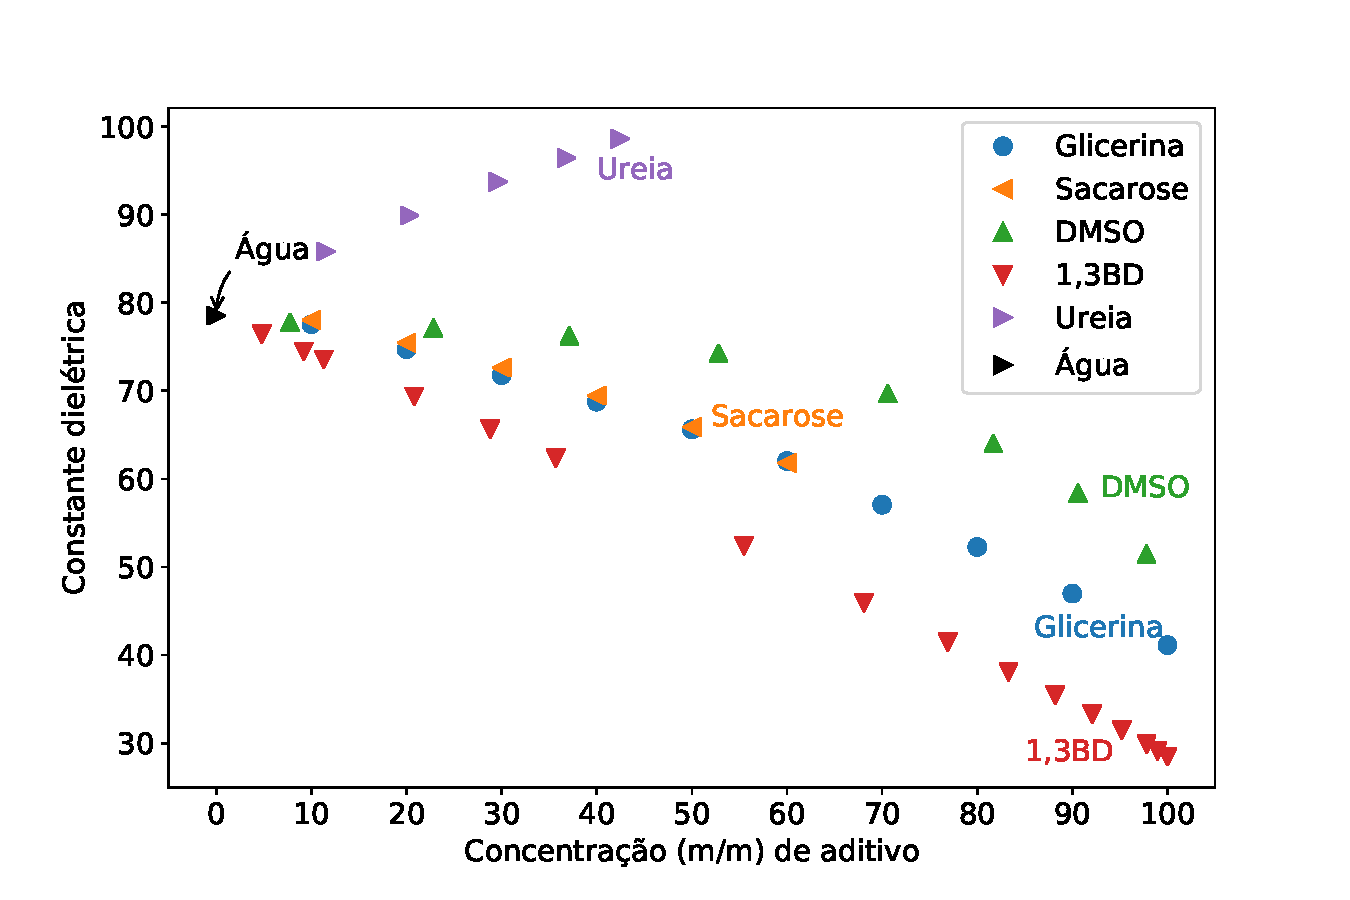
\includegraphics[width=0.7\textwidth]{imagens/propriedades/cte_dieletrica}
			\caption{Constante dielétrica em função da concentração de aditivo}  % todo: colocar quais são a 20°C e quais a 25°C
			\label{fig:cte_dieletrica}
		\end{figure}
	
		Não há variação entre o comportamento da sacarose e glicerina, e o DMSO praticamente não afeta a constante dielétrica na faixa de concentração estudada. O 1,3BD possui sempre os menores valores de \(\varepsilon\), o que indica que nessas soluções há a menor dessorção de contraíons da superfície micelar. O aditivo que afeta a constante dielétrica mais diferentemente dos outros é a ureia, que aumenta \(\varepsilon\). Isso se mostrará crucial para explicar seu comportamento diferenciado.
	
		Da mesma maneira que o índice de refração, os parâmetros dos ITCs serão comparados com a constante dielétrica do meio para tentar observar algum padrão.
		
		\begin{figure}[h]
			\begin{subfigure}[t]{0.5\textwidth}
				\centering
				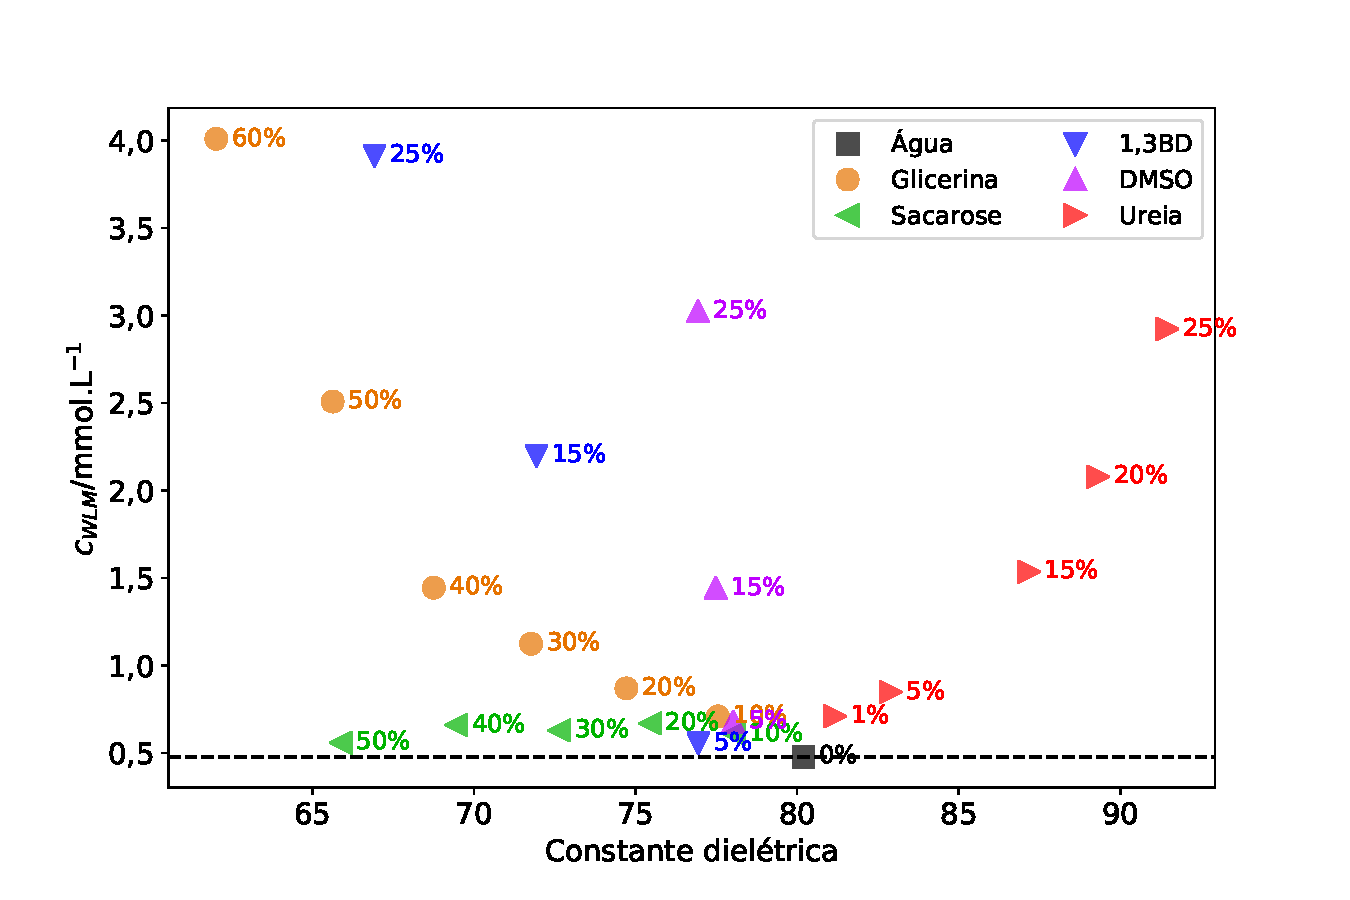
\includegraphics[width=\textwidth]{imagens/itc/Cwlm_por_eps}
				\caption{\cwlm}
				\label{fig:cwlm_por_eps}
			\end{subfigure} %
			\begin{subfigure}[t]{0.5\textwidth}
				\centering
				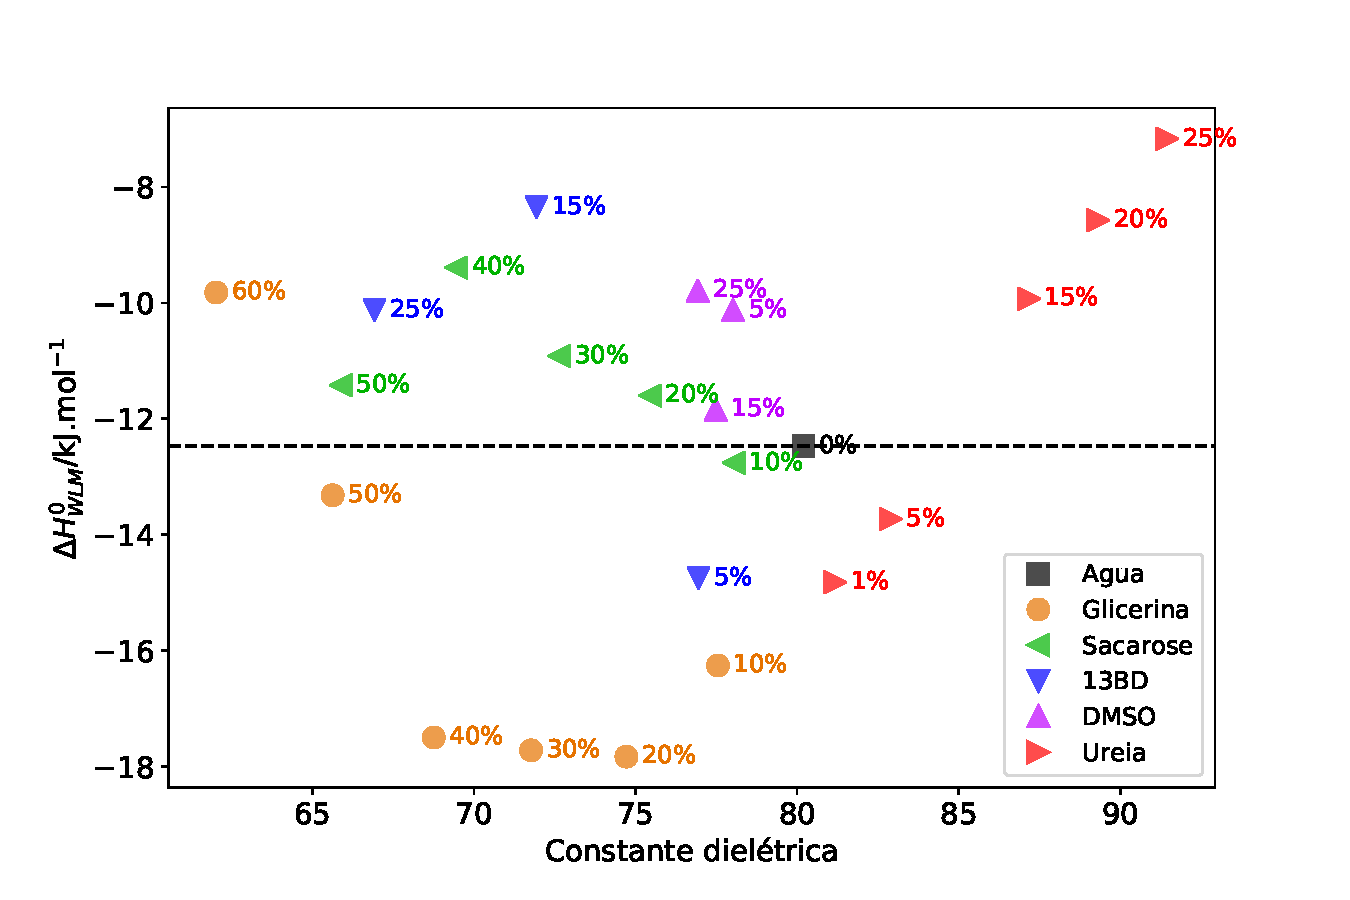
\includegraphics[width=\textwidth]{imagens/itc/DHwlm_por_eps}
				\caption{\DHwlm}
				\label{fig:dhwlm_por_eps}
			\end{subfigure}
			
			\caption{\cwlm{} e \DHwlm{} em função da constante dielétrica \(\varepsilon\).}
			\label{fig:cwlm_dhwlm_por_eps}
		\end{figure}
		
		\begin{figure}[h]
			\begin{subfigure}[t]{0.5\textwidth}
				\centering
				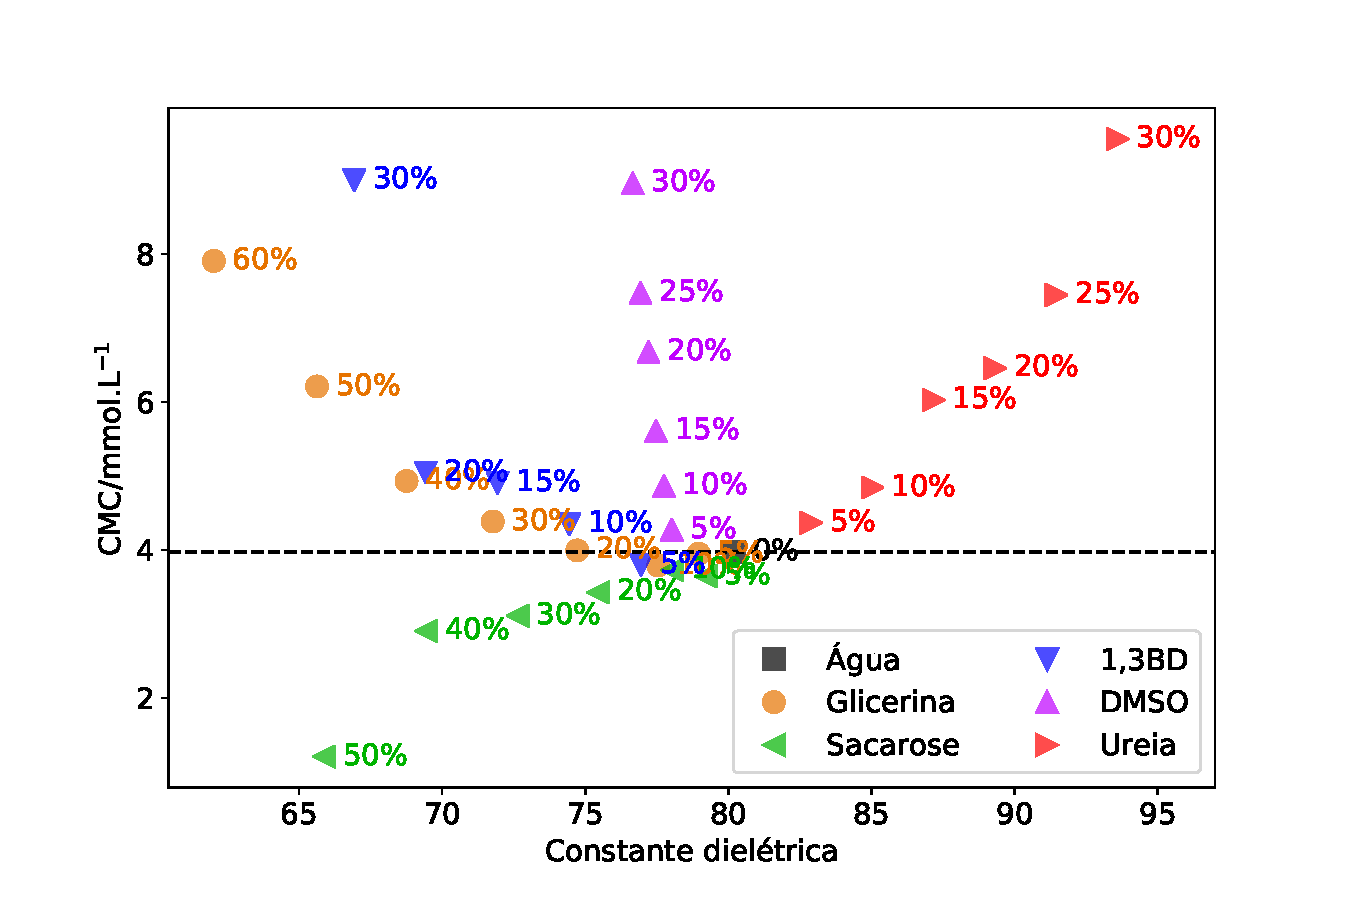
\includegraphics[width=\textwidth]{imagens/itc/CMC_por_eps}
				\caption{\cmc}
				\label{fig:cmc_por_eps}
			\end{subfigure} %
			\begin{subfigure}[t]{0.5\textwidth}
				\centering
				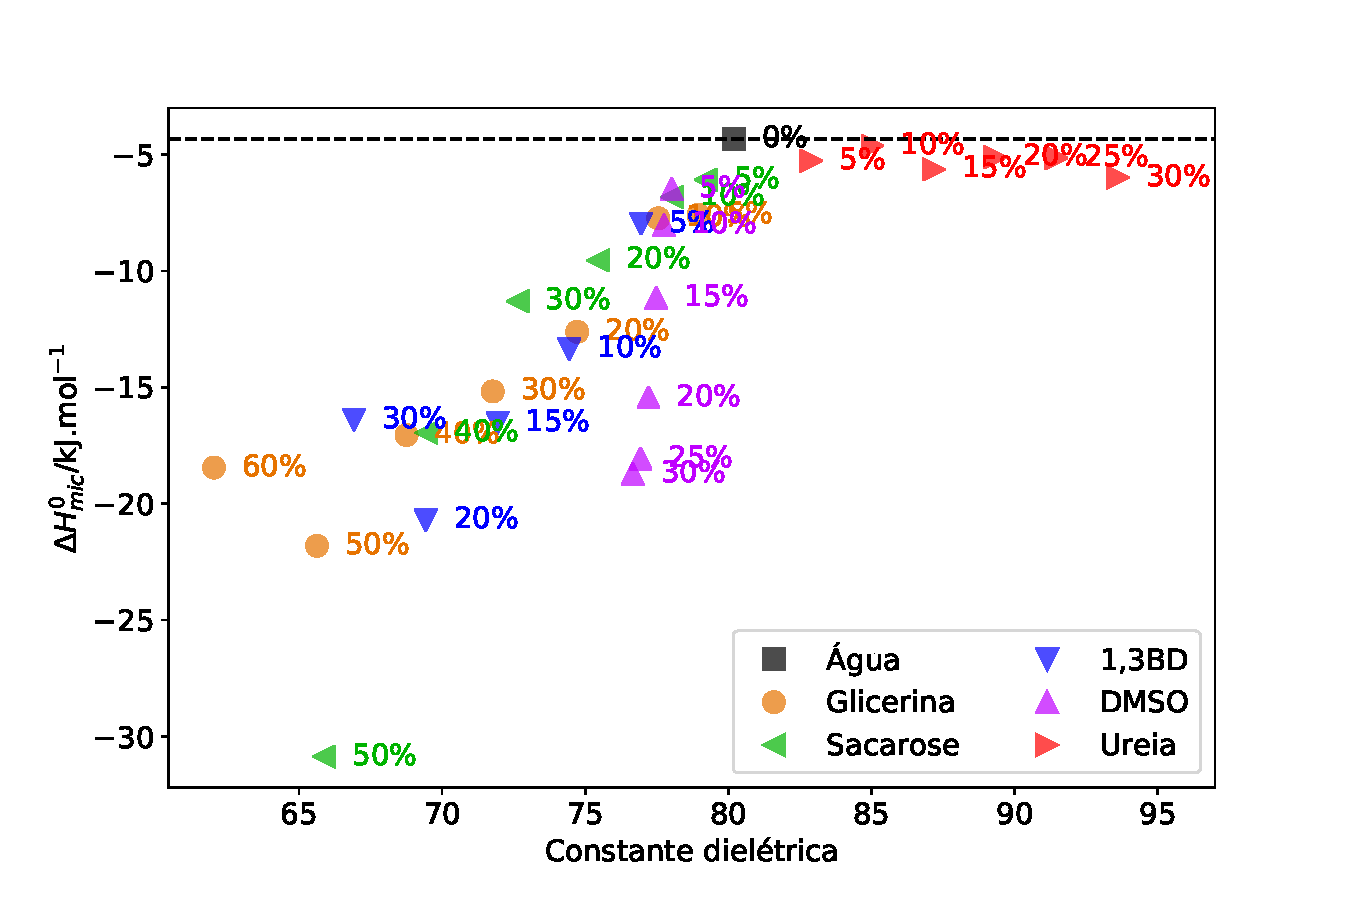
\includegraphics[width=\textwidth]{imagens/itc/DH_por_eps}
				\caption{\DHmic}
				\label{fig:dh_por_eps}
			\end{subfigure}
			\caption{\cmc{} e \DHmic{} em função da constante dielétrica \(\varepsilon\) do meio.}
			\label{fig:cmc_dh_por_eps}
		\end{figure}
		
		Algumas observações podem ser feitas quanto aos resultados observados. Aparentemente todos os aditivos possuem uma divergência única do ponto inicial, água, não havendo muita correlação entre eles, com exceção da \DHmic{}, onde a glicerina, sacarose e 1,3BD aparentam seguir uma tendência semelhante. A ureia, em todos os casos, diverge pois seu valor de constante dielétrica aumenta. O DMSO não afeta grandemente \(\varepsilon\), mas tanto as concentrações quanto entalpias são fortemente afetadas pelo aumento de sua concentração. Isso indica que a constante dielétrica, por si só, também não consegue explicar os fenômenos observados. Porém, ela é necessária para capturar a divergência observada com a ureia.
		
		% todo: mencionar reologia na seção do epsilon
		
		\FloatBarrier
		\section{Coesão do solvente e Parâmetro de Gordon}  % todo: falar sobre estruturação do solvente aqui
		
		Devido à incapacidade dos outros parâmetros explicarem o comportamento reológico e calorimétrico, procuramos por outras propriedades que possam estar relacionadas. Vendo trabalhos anteriores, pensamos na coesão do solvente para explicar o comportamento reológico e calorimétrico. Solventes bastante estruturados, como a água, diminuem a \cmc{} devido ao aumento da penalidade entrópica. Além disso, estipulamos que solventes melhor estruturados devem dificultar a locomoção das micelas gigantes durante os processos de reptação, aumentando a viscosidade aparente. A partir disso, foram coletadas informações sobre a coesão dos solventes utilizados.
		
		Glicerina na concentração de 43\% m/m possui uma probabilidade reduzida de ligações de hidrogênio, portanto a percolação da rede de ligações de hidrogênio é reduzida. Já açúcares são desestruturadores em baixas concentrações e estruturadores em altas. Para a glicose, a estruturação acontece em torno de 25-30\% m/m, já outros estudos mencionam 37\% m/m. Sacarose foi descrita em trabalhos anteriores como aditivo para aumento da separação interlamelar, semelhante à glicerina. É possível que a sacarose afete as micelas e não as bicamadas devido à maior área de contato das micelas com o solvente. Além disso, a reologia observa a dinâmica das micelas ao fluir pelo solvente, já a distância interlamelar é uma propriedade estática, e seria melhor comparada com uma distância intermicelar média.
		
		DMSO foi demonstrado como um agente desestruturador em altas concentrações e estruturador em baixas, e essas propriedades foram descritas como fracas frente à capacidade do DMSO em solubilizar moléculas de surfactante. % todo: o que significa isso exatamente?
		Já o papel da ureia é inconclusivo de acordo com a literatura, com vários mecanismos propostos em estudos. % todo: mencionar os três mecanismos.
		
		Para seguir a lógica das discussões na outra seção, é necessário levantar uma propriedade que traduza o conceito de coesão do solvente para um número mensurável. O parâmetro de Gordon já foi utilizado na literatura com esse propósito, então ele será utilizado neste trabalho. Não foi utilizado o parâmetro de densidade de energia coesiva \(c\) devido à dificuldade de medir esse parâmetro. Porém, é necessário reforçar que \(G\) não traduz perfeitamente o conceito de estruturação, e será utilizado mais como uma maneira para facilitar a discussão. O parâmetro de Gordon já foi definido na equação \ref{eqn:Gordon}.
		
		Amostras com as composições desejadas foram preparadas e suas tensões superficiais foram medidas em quintuplicatas. As tensões obtidas estão na figura \ref{fig:tensao_superficial_por_conc} e os valores do parâmetro de Gordon obtidos estão na figura \ref{fig:param_gordon_por_conc}.
		
		\begin{figure}[h]
			\centering
			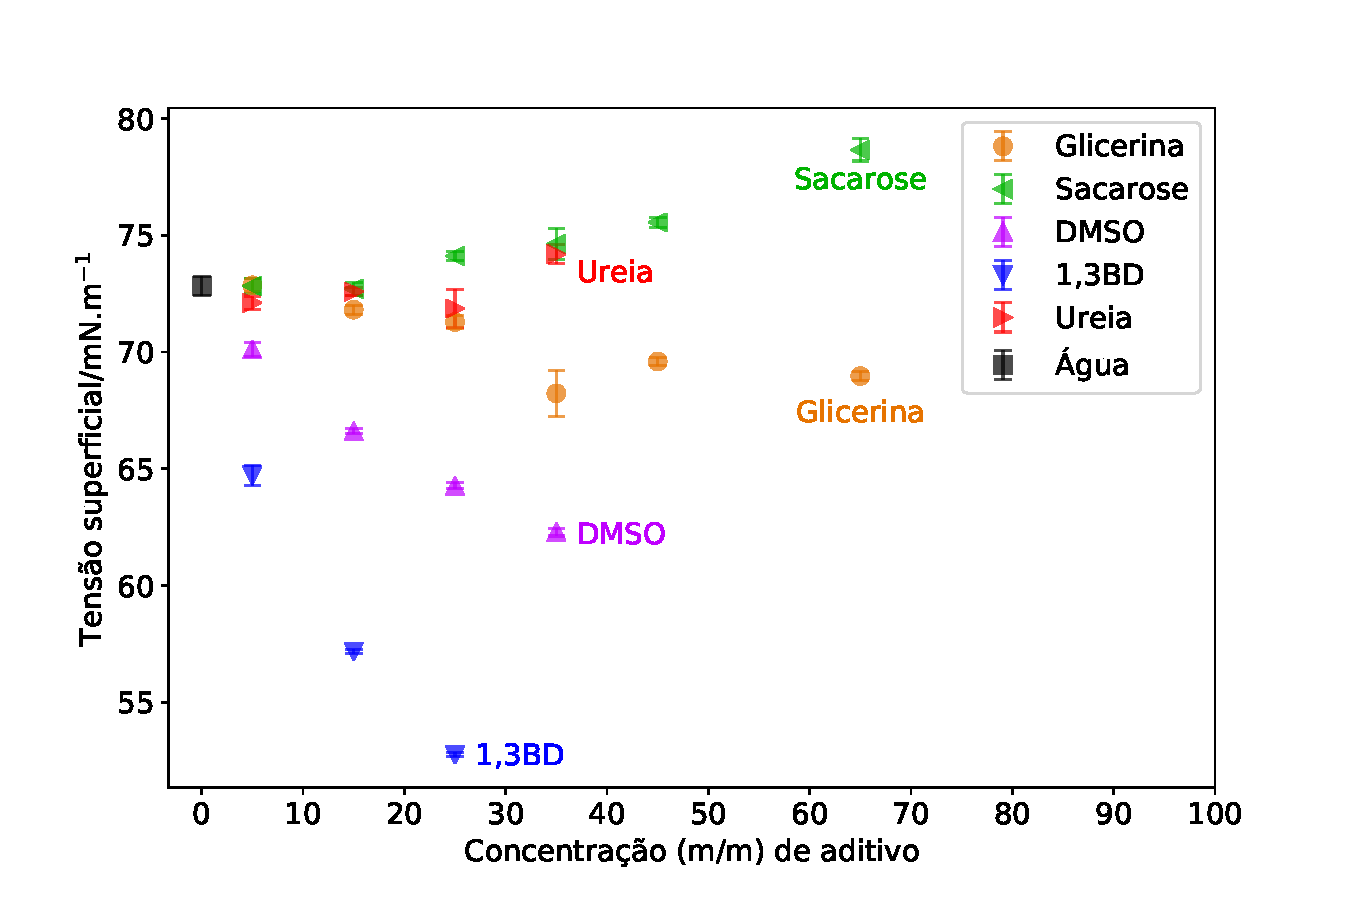
\includegraphics[width=0.7\textwidth]{imagens/propriedades/tensao_superficial}
			\caption{Tensão superficial de misturas binárias dos aditivos em água}
			\label{fig:tensao_superficial_por_conc}
		\end{figure}
		
		\begin{figure}[h]
			\centering
			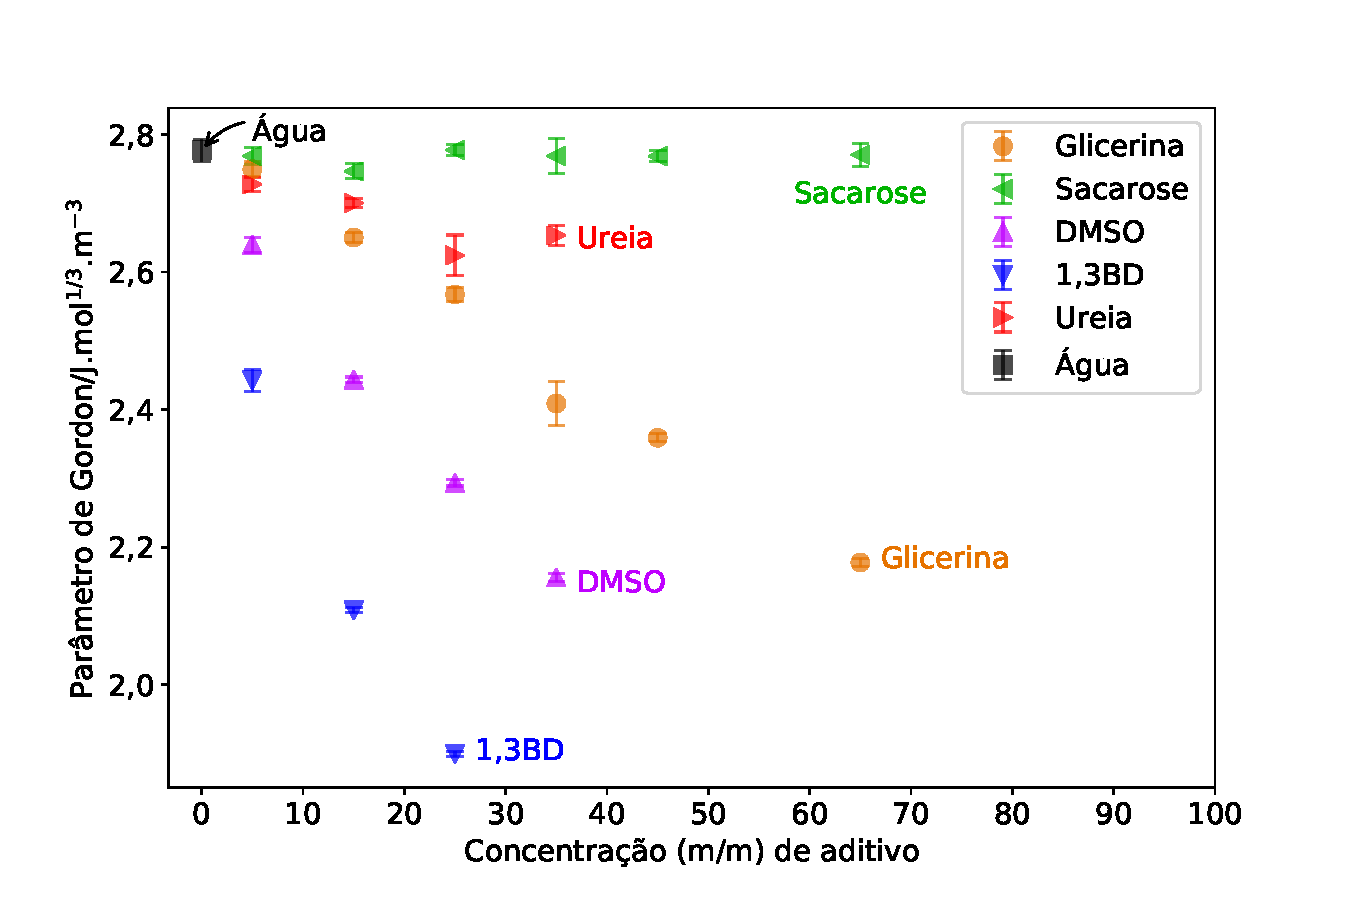
\includegraphics[width=0.7\textwidth]{imagens/propriedades/param_gordon}
			\caption{Parâmetro de Gordon das misturas binárias dos aditivos em água}
			\label{fig:param_gordon_por_conc}
		\end{figure}
		
		Podemos observar que os dois gráficos possuem basicamente o mesmo formato. A maior alteração ocorre devido à divisão pelo volume molar, onde a alta massa da sacarose mascara o aumento de sua tensão superficial, tornando os valores de \(G\) constantes. Essa divisão também diferencia as curvas de ureia e sacarose.
		
		Pelo posição relativa das retas observadas para cada aditivo, podemos construir a seguinte correlação de estruturação do solvente:
		
		\begin{equation*}
			\textrm{1,3BD} < \textrm{DMSO} < \textrm{Glicerina} < \textrm{Ureia} < \textrm{Sacarose}
		\end{equation*}
		
		Essa sequência possui grande correlação com o comportamento reológico (com exceção da ureia). 1,3BD, que possui a menor estruturação, reduz mais fortemente a viscosidade das micelas. Já a sacarose praticamente não afetou a estruturação do solvente, e também não afetou muito a viscosidade. Como mencionado, a ureia é uma exceção devido à grande alteração na constante dielétrica, que deve dessorver moléculas de salicilato das micelas e aumentar sua carga. Isso faz com que o mecanismo principal de relaxação seja a reptação na faixa de concentração estudada, então a viscosidade é sempre alta.
		
		Para compreender o efeito do parâmetro de Gordon nas titulações, foram criadas figuras comparativas, da mesma maneira que nas seções anteriores. Os comparativos para a formação de micelas gigantes e micelas esféricas estão nas figuras \ref{fig:cwlm_dhwlm_por_g} e \ref{fig:cmc_dh_por_g}, respectivamente.
		
		\begin{figure}[h]
			\begin{subfigure}[t]{0.5\textwidth}
				\centering
				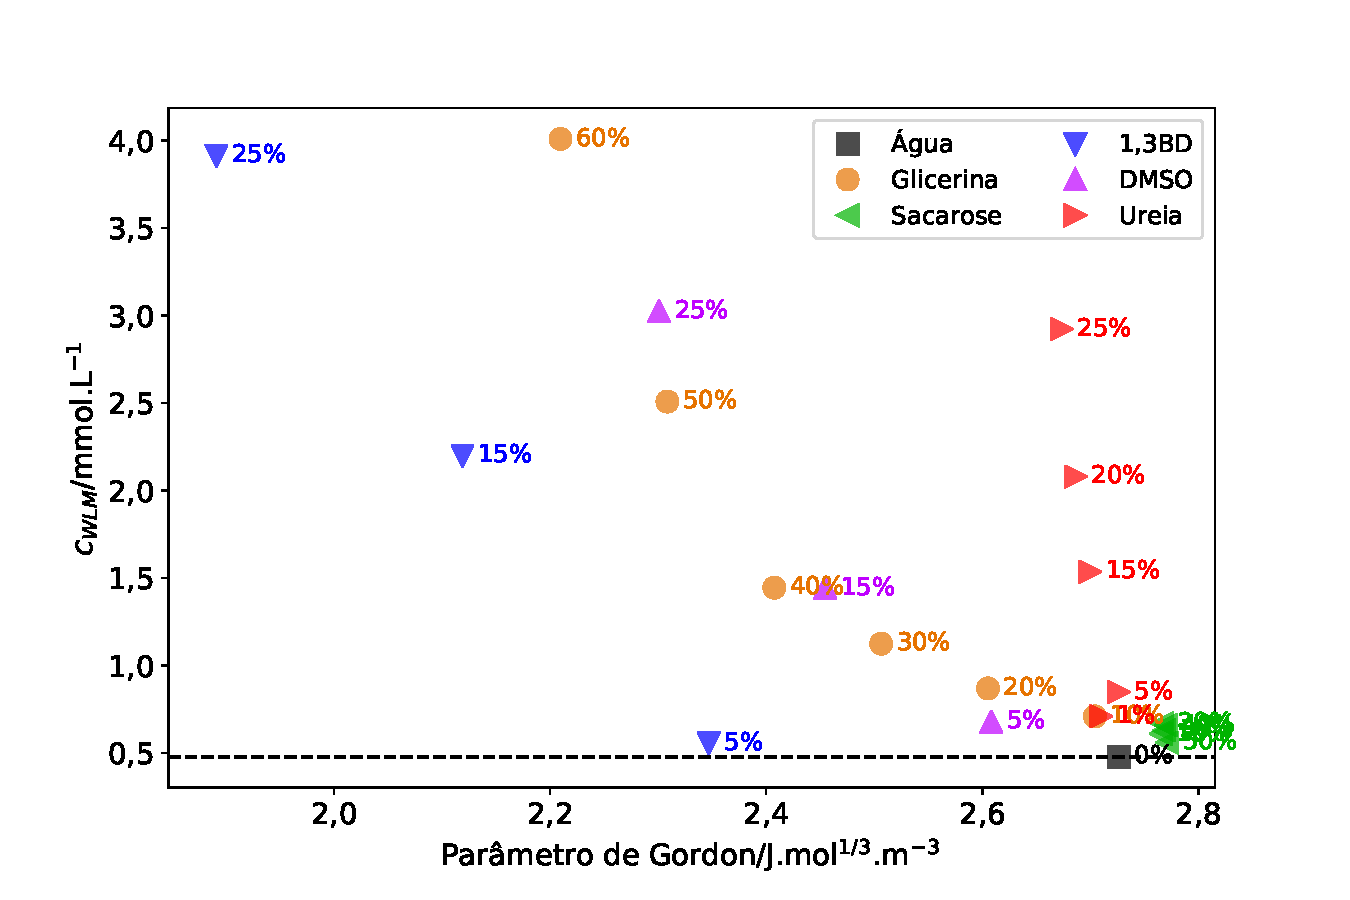
\includegraphics[width=\linewidth]{imagens/itc/Cwlm_por_G}
				\caption{\cwlm}
				\label{fig:cwlm_por_g}
			\end{subfigure} %
			\begin{subfigure}[t]{0.5\textwidth}
				\centering
				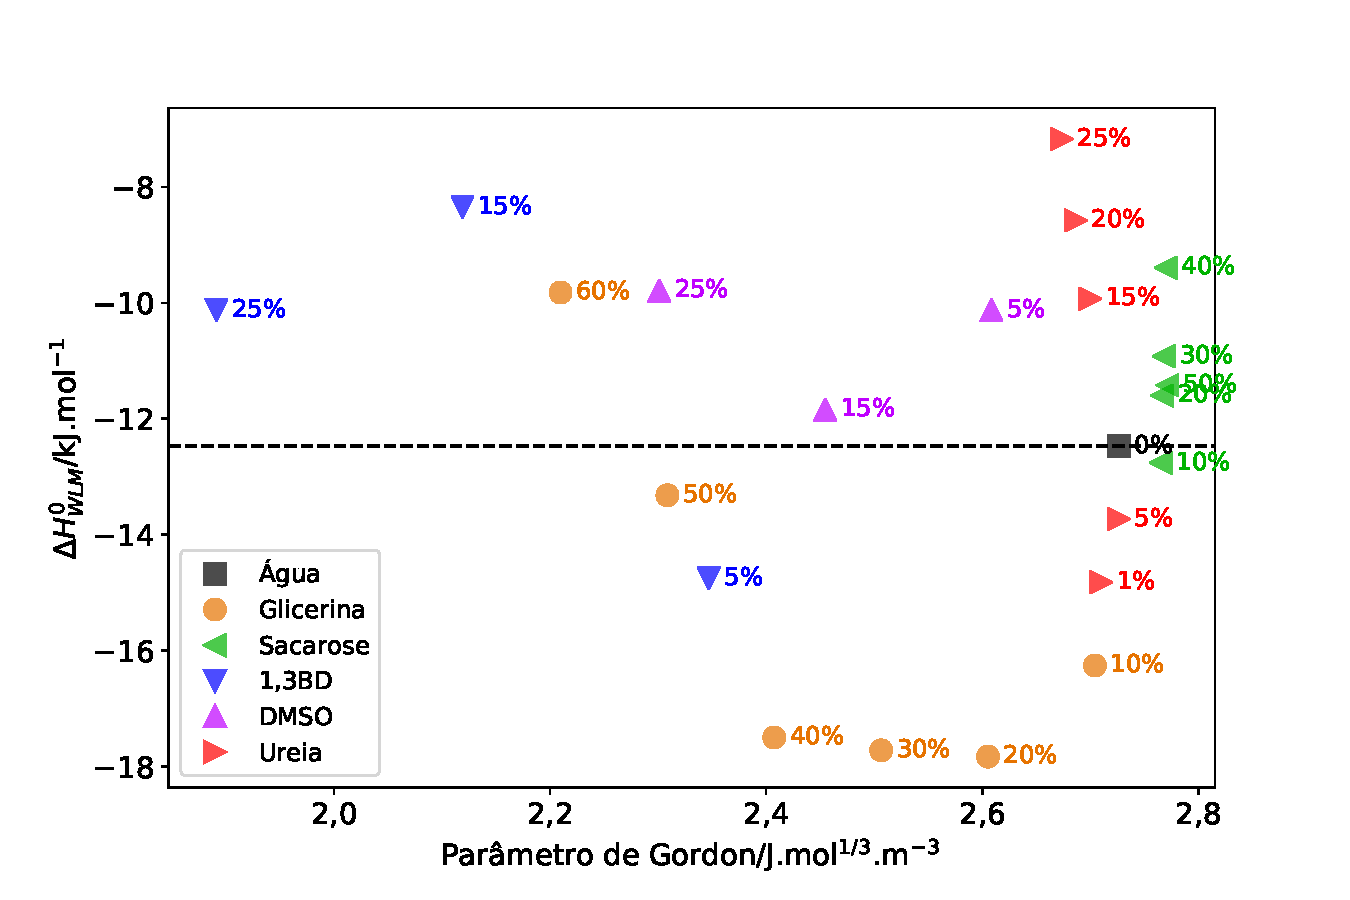
\includegraphics[width=\textwidth]{imagens/itc/DHwlm_por_G}
				\caption{\DHwlm}
				\label{fig:dhwlm_por_g}
			\end{subfigure}
			\caption{\cwlm{} e \DHwlm{} em função do parâmetro de Gordon}
			\label{fig:cwlm_dhwlm_por_g}
		\end{figure}
		
		\begin{figure}[h]
			\begin{subfigure}[t]{0.5\textwidth}
				\centering
				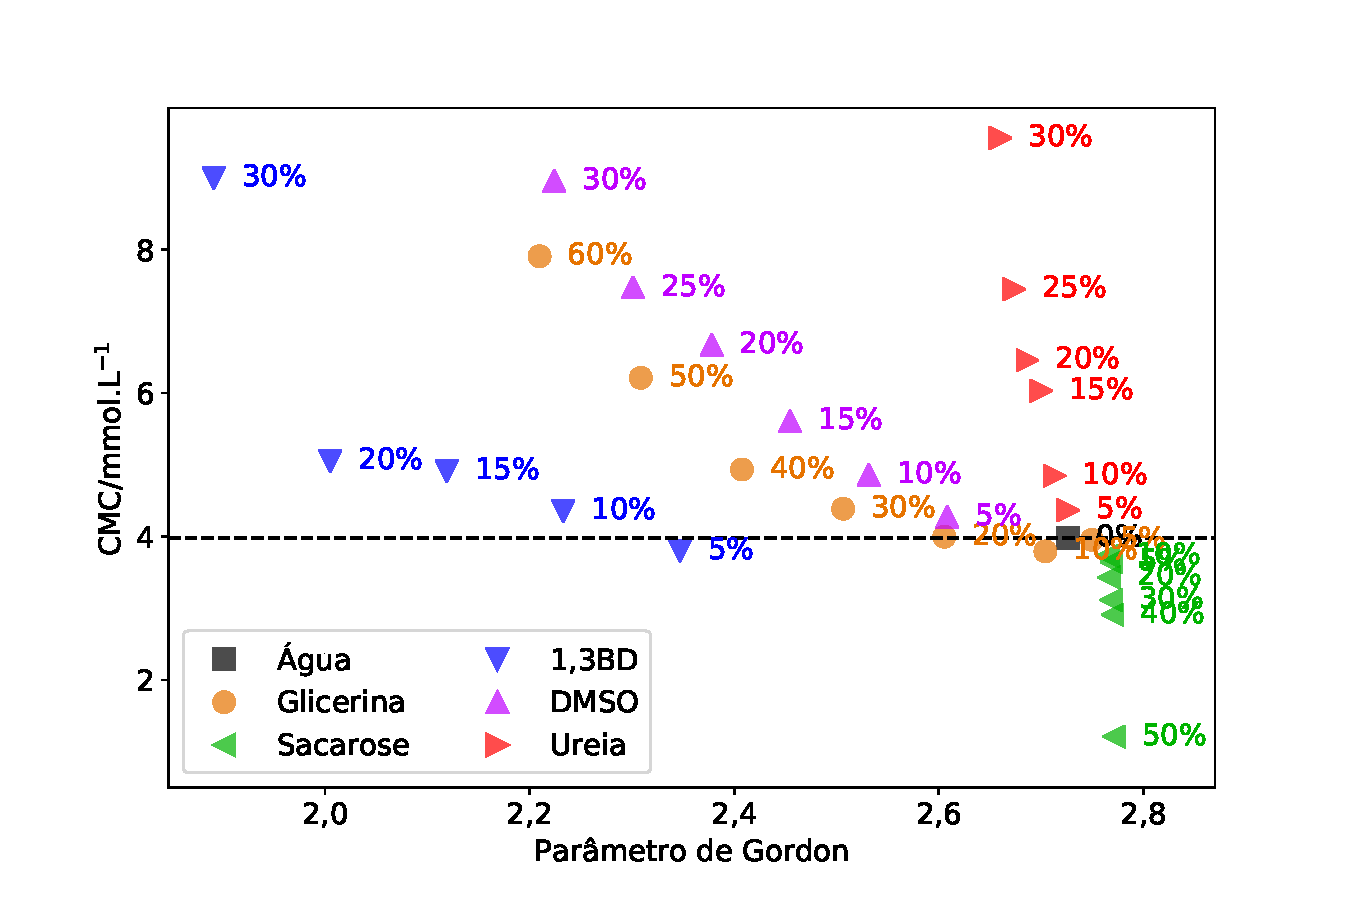
\includegraphics[width=\textwidth]{imagens/itc/CMC_por_G}
				\caption{\cmc}
				\label{fig:cmc_por_g}
			\end{subfigure} %
			\begin{subfigure}[t]{0.5\textwidth}
				\centering
				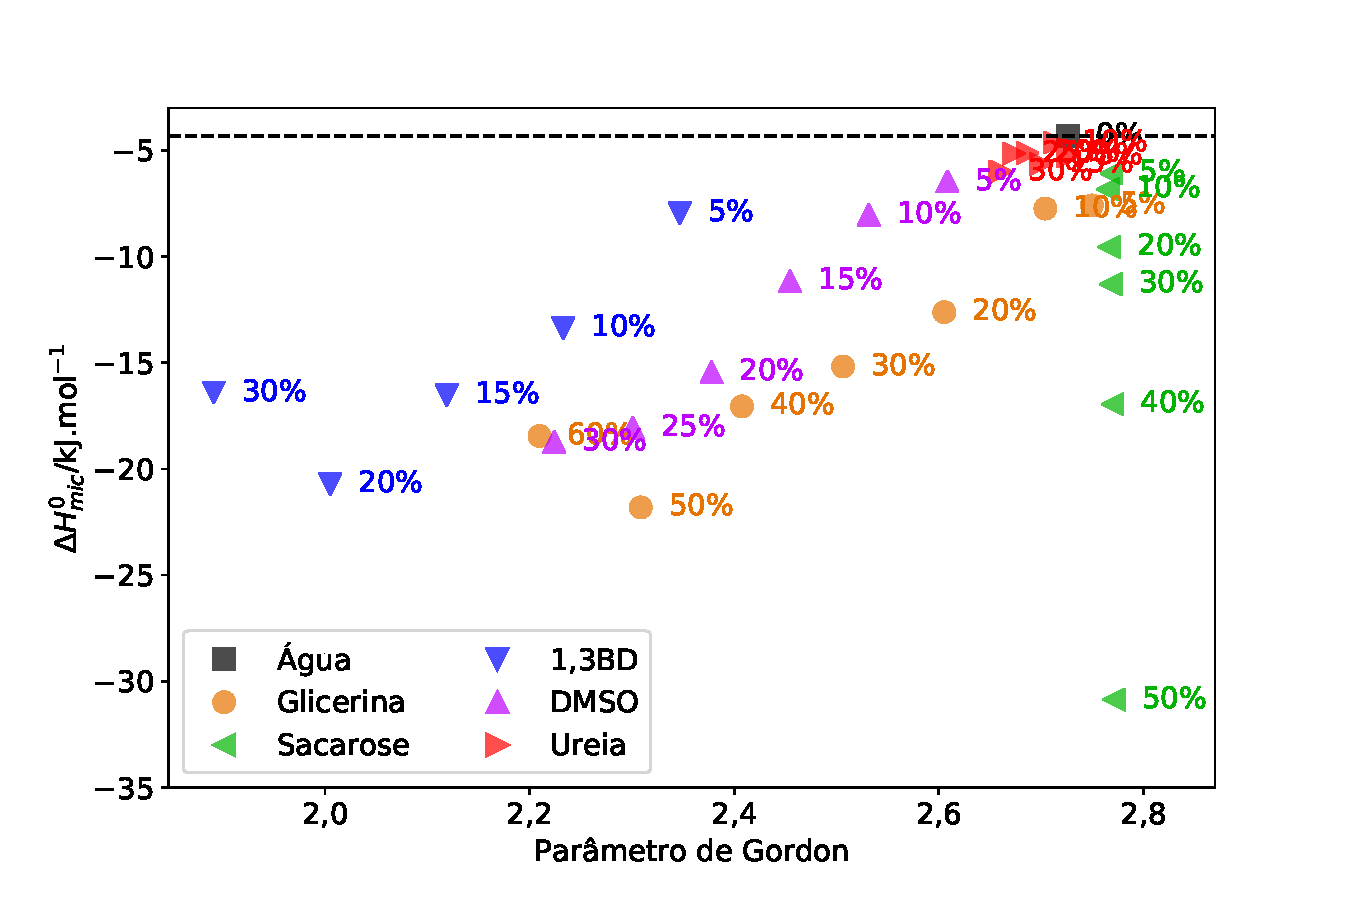
\includegraphics[width=\linewidth]{imagens/itc/DH_por_G}
				\caption{\DHmic}
				\label{fig:dh_por_g}
			\end{subfigure}
			\caption{\cmc{} e \DHmic{} em função do parâmetro de Gordon}
			\label{fig:cmc_dh_por_g}
		\end{figure}
		
		Pela inclinação das retas observadas nas figuras \ref{fig:cwlm_por_g} e \ref{fig:cmc_por_g}, podemos observar o quão forte é o efeito de uma mudança no parâmetro de Gordon do aditivo específico na concentração de micelização. A ureia possui o efeito mais forte, onde uma pequena variação de \(G\) aumentou muito a \cmc, porém isso se deve principalmente ao aumento de \(\varepsilon\). Sacarose não afetou a \cwlm{} e diminuiu a \cmc, pelas razões já discutidas. Os outros três aditivos seguem uma tendência semelhante, onde uma diminuição de \(G\) resulta no aumento gradativo de \cwlm{} e \cmc. Pela inclinação, 1,3BD possui o efeito mais brando na \cwlm, mas se a concentração de aditivo for levada em consideração também, vemos que seu efeito é bastante forte, atingindo a \cwlm{} de 4 \mM{} com 25\% de aditivo, comparado com glicerina, que atingiu essa concentração com 60\%. Interessantemente, até 20\%, o efeito do 1,3BD na \cmc{} é bastante pequeno, menor que o DMSO, e há um salto em 30\%, equiparando-se ao DMSO.
				
		As \DHwlm{} não possuem uma ordenação clara. Ureia aparenta ter comportamentos divergentes entre soluções de concentrações baixas (\(<\) 15\%) e altas (\(\ge\) 15\%). Já a \DHmic{} possui padrões, como os valores de ureia agrupados, pois não há salicilato para ser dessorvido. Glicerina e DMSO novamente possuem um comportamento relativemente próximo, e 1,3BD tem o menor efeito na entalpia por variação de \(G\). A sacarose diminui a \DHmic{} e a \cmc{}, apesar de não afetar \(G\), indicando que seu papel está relacionado com a interação com as micelas, não somente seu efeito no solvente.
		
		A correlação do parâmetro de Gordon é especialmente forte com o comportamento reológico, e há algumas correlações que podem ser feitas com a calorimetria. Deve ser enfatizado que esse parâmetro, por si só, também não explica o comportamento completo. É necessário combinar todas essas considerações para entender o sistema.
		\FloatBarrier
		
		\section{Interação dos aditivos com a superfície micelar}
		% todo: pensar em desmembrar essas considerações e espalhar nas outras seções
		
		Uma propriedade importante que deve receber enfoque é a interação dos aditivos com a superfície micelar. Aditivos que interagem fortemente afetam muito os processos de autoassociação, como demonstra o salicilato de sódio. Efeitos semelhantes, mas menos intensos, podem complementar os parâmetros levantados até o momento.
		
		Estudos da influência de álcoois lineares na viscosidade de micelas gigantes de C\textsubscript{16}TASal e CPySal mostraram que quando álcoois de cadeia curta interagiam com a superfície micelar, agiam como um cossolvente e diminuiam o comprimento das micelas, logo diminuindo sua viscosidade. Caso 1,3-BD se comporte de maneira similar, esse é mais um efeito que pode resultar nas quedas fortes da viscosidade. Um estudo mostra que o 1,3-BD interage como cosurfactante em cristais líquidos, o que reforça a teoria de seu efeito em micelas gigantes. Além disso, o 1,3BD pode interagir com os grupos metil na superfície micelar, diminuindo a atração entre as micelas que ocorre devido a esses grupos, o que diminuiria a viscosidade. A glicerina, por ser mais polar, possivelmente não tem o mesmo efeito que 1,3BD, logo é menos eficaz em diminuir a viscosidade ou aumentar a \cmc. O DMSO pode se solubilizar na superfície micelar e interagir com os grupos metila, pois é menos polar que os outros aditivos, e isso pode resultar em uma diminuição maior na viscosidade. 
		
		%Ureia interage fortemente com a superfície micelar, mas não como agente intercalante. % todo: verificar o artigo na ACS Omega sobre o que eu falo sobre isso.
	%	A concentração de ureia na superfície é cerca de 10-30\% menor do que no seio da solução. 
		
		% todo: refs
		A sacarose diminui a \cmc{} de outros surfactantes, como SDS, CTAB e Brij 35, pela interação de suas hidroxilas com a superfície micelar reduzindo a repulsão, e pela estruturação do solvente. Logo, a diminuição de \(n\) e \(\varepsilon\), que deveriam aumentar a \cwlm{}, são compensadas e a \cwlm{} é mantida. Não há uma diminuição de \cwlm, como houve de \cmc, pois o salicilato interage mais fortemente com a superfície micelar, deslocando as hidroxilas da sacarose, logo seu efeito é principalmente na estruturação do solvente.
		
		% todo: pensar em colocar uma seção falando sobre o DeltaG.
		
		\section{Correlações simultâneas dos parâmetros com \cmc{} e \DHmic}
		% todo: colocar que esse tipo de análise já foi utilizada para tentar descrever padrões em solventes
		
		Até este momento, foram feitas correlações dos parâmetros do solvente com as propriedades calorimétricas mensuradas somente um a um, com raros casos explicados considerando-se outros parâmetros simultaneamente. Seria interessante tentar correlacionar todas essas propriedades simultaneamente, ou seja, realizar uma análise multivariada.
		
		Esse tipo de análise, tanto utilizando métodos de regressão linear múltipla, ou ordinária (\emph{OLS}), e análise de componentes principais (\emph{PCA} e \emph{PLS}) são principalmente utilizados na área da química analítica, chamada de Quimiometria, mas também são utilizadas para classificar solventes orgânicos. %todo: refs
		Uma das necessidades para esse tipo de análise é que as variáveis sejam verdadeiramente independentes umas das outras, aditivas e relevantes ao problema em questão. % todo: ref [144] do capítulo 3, um livro que eu não achei
		
		Estudos de classificação dos solventes utilizam os parâmetros já mencionados, e vários outros, como pontos de ebulição, coeficientes de partição, volume molar, constante dielétrica, índice de refração, energia de HOMO e LUMO, parâmetro \(E_T(30)\) obtidos a partir de uma sonda solvatocrômica, parâmetro de Hildebrand e momento de dipolo. % todo: colocar algumas referências aqui, como [Chastrette 1985]
		Não necessariamente esses parâmetros são independentes, o que resultaria numa redução da dimensão dos dados.
		
		O objetivo desta seção é facilitar a interpretação dos resultados calorimétricos % todo: e reológicos?
		através dos parâmetros da solução escolhidos (\(n\), \(\varepsilon\), \(G\)), e não realizar uma descrição quimiométrica completa, nem atribuir muitos significados físicos aos coeficientes encontrados. Não serão mostrados os resultados desses ajustes para reologia (utilizando a viscosidade como variável dependente, os parâmetros e concentração de NaSal como variável dependente) e calorimetria de micelas gigantes (utilizando \cwlm{} e \DHwlm{} como variáveis dependentes e os parâmetros como variáveis dependentes) pois não foi observado um ajuste bom.
		
		Inicialmente, será utilizado um método quimiométrico bastante empregado, o PLS (\emph{Partial Least Squares}), depois será utilizado um método de regressão linear mais simples, e por último as misturas binárias serão organizadas em grupos de acordo com suas similaridades, através de um dendrograma.
		
		\subsection{PLS}
		
		Foram feitas análises de PLS (\emph{Partial Least Squares}) com o índice de refração, constante dielétrica e parâmetro de Gordon para tentar prever a \cmc{} e a \DHmic. Utilizou-se dois componentes principais (de 3) em ambos os casos, os dados foram autoescalados de modo a garantir que todas as parâmetros tenham o mesmo peso no modelo final. Utilizou-se validação cruzada com 1 elemento, e sem validação cruzada, e o vetor de previsão permaneceu igual. Essas análises foram realizadas com o software Pirouette 3.11, e comparadas com uma análise foi feita utilizando pacote \emph{sklearn}, em Python. Esse pacote é livre, ao contrário do Pirouette, então qualquer um pode reproduzir essas análises. Os resultados foram absolutamente iguais, então não serão mostradas as figuras resultantes de ambos os métodos, somente daqueles obtidos no Pirouette. As retas de \cmc{} e \DHmic{} medidos por \cmc{} e \DHmic{} observados estão presentes nas figuras \ref{fig:pls_cmc_pirouette} e \ref{fig:pls_dh_pirouette}, respectivamente.
		
		\begin{figure}[h]
			\centering
			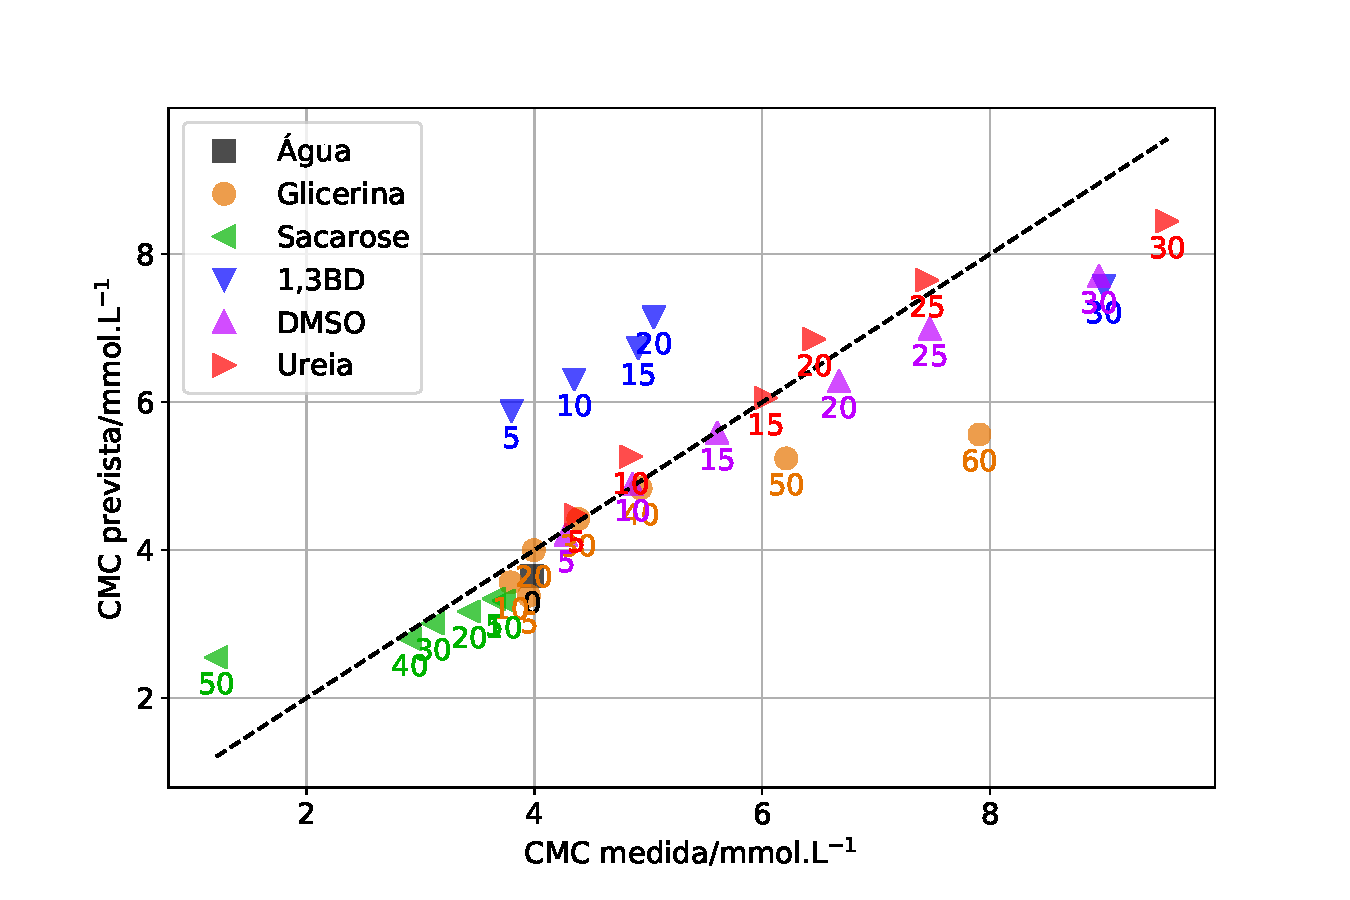
\includegraphics[width=0.7\textwidth]{imagens/itc/PLS_cmc_pirouette}
			\caption{Comportamento do modelo de \cmc{} criado por PLS, mostrando a correlação entre os valores observados e previstos. A reta preta tracejada mostra o modelo perfeito, onde há uma relação 1:1 entre o observado e o previsto. A reta vermelha mostra o modelo criado, junto com a qualidade do ajuste.}
			\label{fig:pls_cmc_pirouette}
		\end{figure}
	
		\begin{figure}[H]
			\centering
			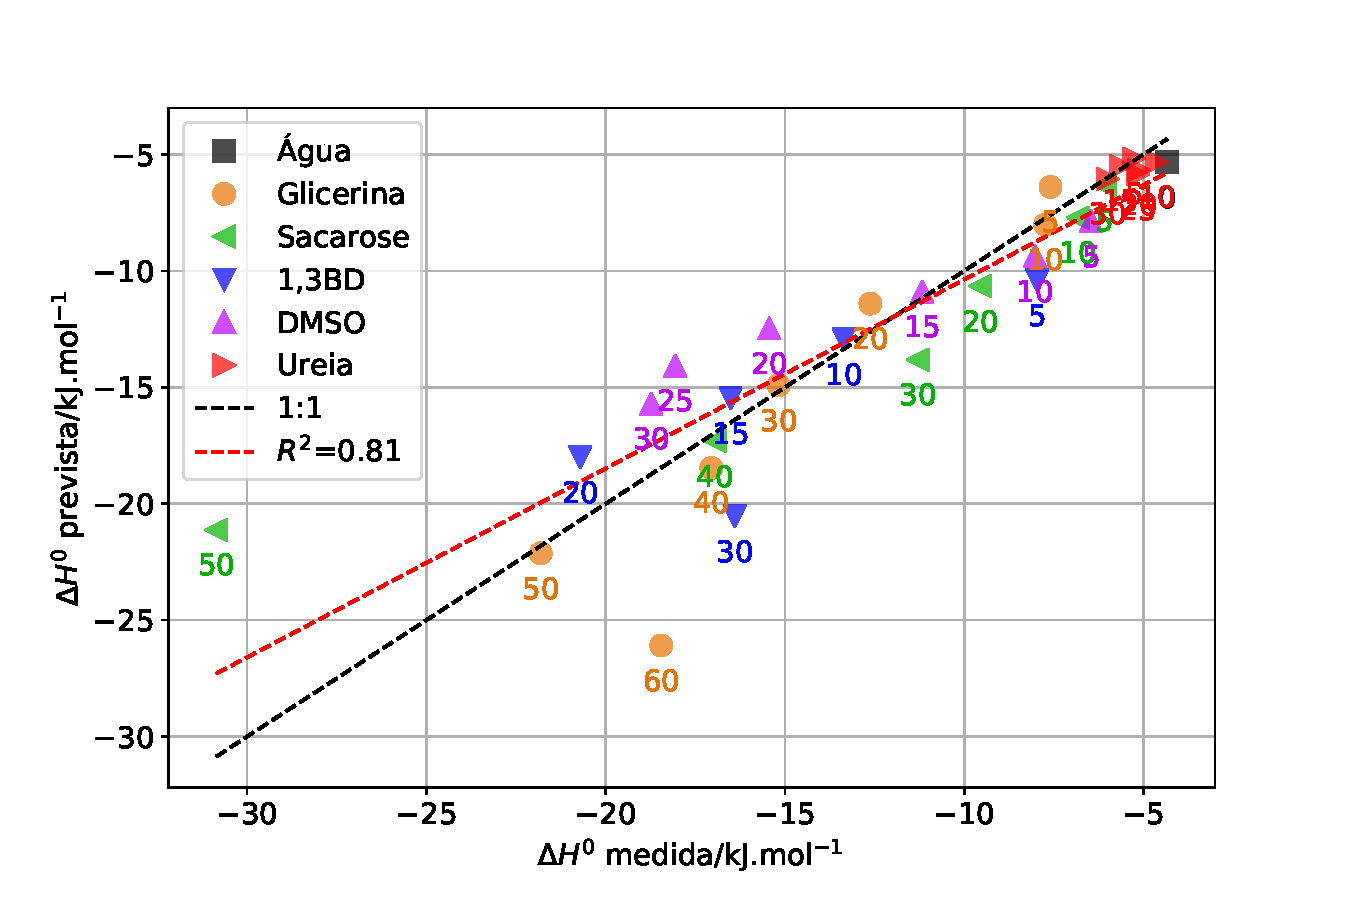
\includegraphics[width=0.7\textwidth]{imagens/itc/PLS_dh_pirouette}
			\caption{Comportamento do modelo de \DHmic{} criado por PLS, mostrando a correlação entre os valores observados e previstos. A reta preta tracejada mostra o modelo perfeito, onde há uma relação 1:1 entre o observado e o previsto. A reta vermelha mostra o modelo criado, junto com a qualidade do ajuste.}
			\label{fig:pls_dh_pirouette}
		\end{figure} 
		
		Pelas curvas de ajuste e do modelo ideal de \cmc, podemos observar que as amostras que mais divergem da região central são aquelas com alta concentração de aditivo, provavelmente porque a divergência entre suas propriedades e de água pura são muito grandes, e o processo de autoassociação é muito alterado. Além disso, observamos que todas as medidas com 1,3BD estão distantes da reta 1:1, e as concentrações de 5 a 20 \% m/m estão paralelas. Isso indica que esse aditivo possui um efeito adicional, aparentemente constante nessa faixa de concentração, que resulta em valores de \cmc{} menores do que o esperado, observando somente os parâmetros escolhidos. Possivelmente, esse é consequência da tendência do 1,3BD de interagir na superfície micelar, diminuir a repulsão e facilitar a autoassociação.
		
		A previsão de \DHmic{} é melhor que de \cmc, e os compostos que mais fogem do modelo são, novamente, as soluções com maior concentração de aditivo. Em especial, temos 50\% de sacarose, 60\% de glicerina e 30\% de 1,3BD.
		
		O código para fazer análise de PLS em Python, e uma figura semelhante à figura \ref{fig:pls_cmc_pirouette} está na listagem \ref{lst:pls_cmc_python}.
		
		\begin{listing}[h]
			\inputminted{python}{./python/pls_cmc_sklearn.py}
			\caption{Código utilizado para gerar a dependência de \cmc{} com os parâmetros estudados, resultando na Fig. \ref{fig:pls_cmc_pirouette}. A tabela de dados utilizada possui em cada linha as misturas utilizadas, suas concentrações em \% m/m, as variáveis dependentes (\cmc{} e \DHmic) e as variáveis independentes (\(n\), \(\varepsilon\), \(G\))}
			\label{lst:pls_cmc_python}
		\end{listing}
		
		O resultado desse modelo é um conjunto de coeficientes que, quando multiplicados pelos parâmetros escolhidos (\(n\), \(\varepsilon\), \(G\)), resultam nas propriedades (\cmc, \DHmic). Os membros do vetor não possuem unidades pois os dados foram autoescalados, então é necessário desfazer o autoescalamento para obter uma equação que utiliza coeficientes com as unidades utilizadas neste trabalho. As equações \ref{eqn:PLS_cmcs} e \ref{eqn:PLS_dhs} possuem tanto as relações em unidades usuais (a) quanto autoescaladas (b) para a \cmc{} e \DHmic, respectivamente. % (\mM, \(kJ.mol^{-1}\), \(J.mol^{-1/3}.m^{-3}\))
				
		\begin{subequations}
			\begin{align}
				\textrm{CMC}               & = -7,206G              + 0,225\varepsilon             + 27,955n            - 31,871  \label{eqn:PLS_cmc}     \\
				\textrm{CMC}_{\textrm{AS}} & = -0,941G_\textrm{AS}  + 0,864\varepsilon_\textrm{AS} + 0,319n_\textrm{AS}           \label{eqn:PLS_cmc_AS}
			\end{align}
			\label{eqn:PLS_cmcs}
		\end{subequations}
		
		\begin{subequations}
			\begin{align}
				\Delta H_\textrm{mic}^0     &= 7,64G              + 0,395\varepsilon             - 119n                + 101  \label{eqn:PLS_dh} \\
				\Delta H_\textrm{mic, AS}^0 &= 0,300G_\textrm{AS} + 0,458\varepsilon_\textrm{AS} - 0,414n_\textrm{AS}         \label{eqn:PLS_dh_AS}
			\end{align}
			\label{eqn:PLS_dhs}
		\end{subequations}
		
		Os coeficientes das equações autoescaladas estão relacionados com o quanto cada parâmetro afeta a propriedade. Em especial, os sinais mostram se um coeficiente aumenta ou diminui a propriedade modelada. Por exemplo, na equação \ref{eqn:PLS_cmc_AS}, o parâmetro de Gordon possui um sinal negativo. Isso significa que um aumento de \(G\) resulta numa diminuição de \cmc, o que está de acordo com a interpretação fornecida para \(G\), que é a coesividade do solvente. Solventes mais coesos resultam em penalidades entrópicas maiores, favorecendo a micelização. A constante dielétrica, por outro lado, promove a dissociação de íons da superfície micelar, logo um aumento de \(\varepsilon\) resulta num aumento de \cmc, pois a repulsão entre os surfactantes é maior. O índice de refração, ou melhor, a diferença entre o índice de refração do meio e do surfactante, está relacionado com a atração entre as moléculas de surfactante. Quanto maior for \(n\), mais próximos são os índices de refração, menor é a atração e maior é a \cmc.
		
		A visualização do efeito desses parâmetros na \DHmic é menos trivial. Para interpretar esse fenômeno, é necessário entender a origem da entalpia de micelização. % todo: pesquisar e colocar aqui.
		Observamos que somente o índice de refração possui um sinal negativo, logo um aumento de \(n\) resulta numa diminuição de \DHmic{} (tornando-se mais negativo). Por outro lado, \(G\) e \(\varepsilon\) mostram que aumentos em seus valores resultam em uma diminuição na amplitude de \DHmic. 
		
		\FloatBarrier
		\subsection{OLS}
		
		Outra metodologia que pode ser utilizada para realizar essas correlações é a dos mínimos quadrados ordinários (\emph{ordinary least squares}, OLS). Esse método é mais simples do que o PLS, pois não ocorre uma decomposição em componentes principais. Neste caso, o ajuste é feito reduzindo-se os mínimos quadrados da equação \ref{eqn:ols_modelo_cmc}.
		
		\begin{equation}
			\textrm{CMC} = a_G \cdot G + a_\varepsilon \cdot \varepsilon + a_n \cdot n + e
			\label{eqn:ols_modelo_cmc}
		\end{equation}
		
		Esse tipo de ajuste é igual ao ajuste de uma equação linear, porém com mais de uma variável independente. Foram feitos ajustes por mínimos quadrados ordinários tanto para a previsão da \cmc{} quanto a \DHmic. Os resultados dos ajustes estão nas figuras \ref{fig:ols_cmc_python} e \ref{fig:ols_dh_python}.
		
		\begin{figure}[h]
			\centering
			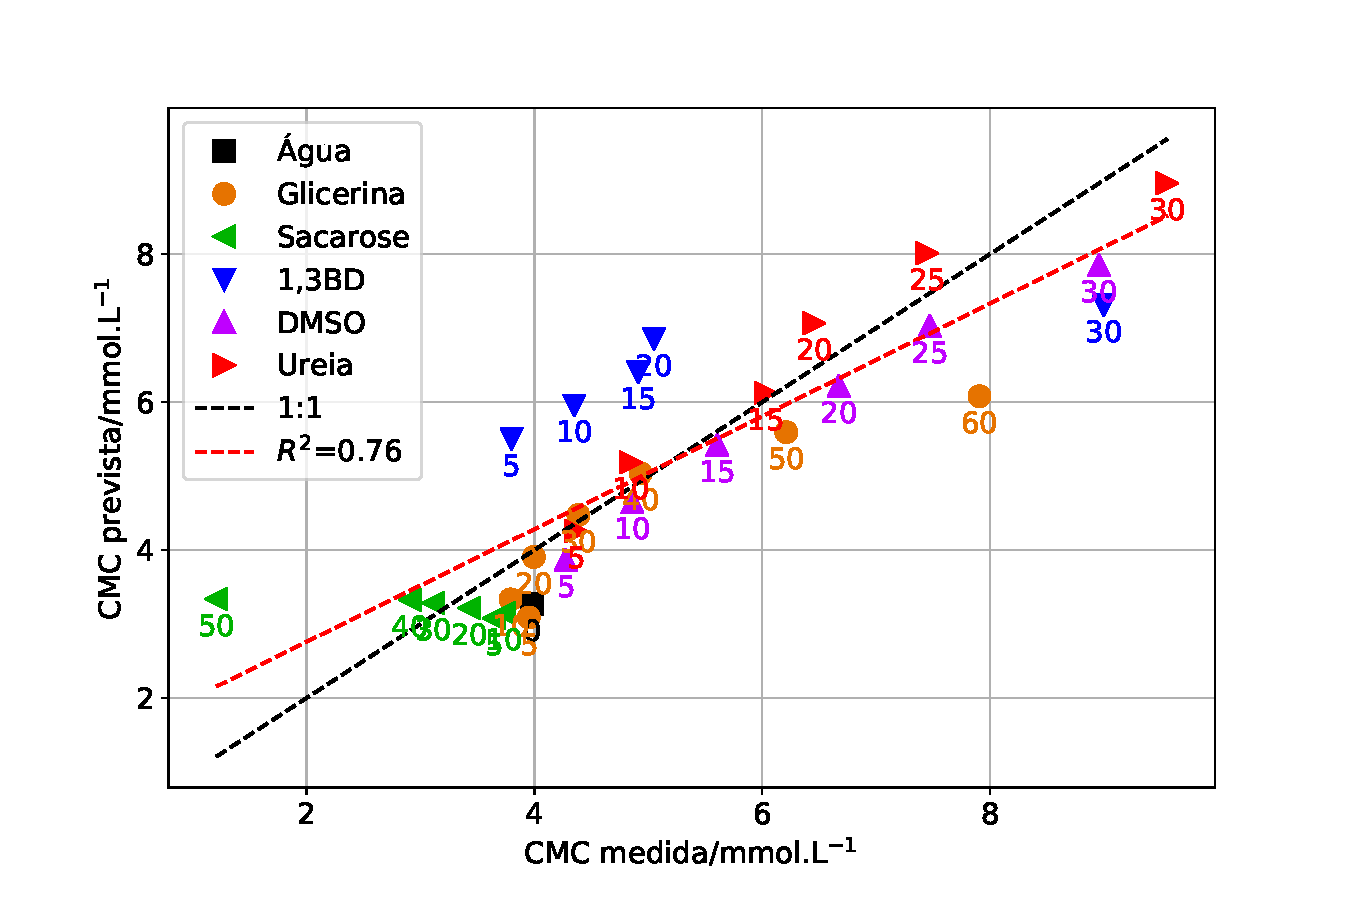
\includegraphics[width=0.7\textwidth]{imagens/itc/ols_cmc_python}
			\caption{Comportamento do modelo de \cmc{} criado por OLS, mostrando a correlação entre os valores observados e previstos. A reta preta tracejada o modelo perfeito, onde há uma relação 1:1 entre o observado e o previsto. A reta vermelha mostra o modelo criado, junto com a qualidade do ajuste.}
			\label{fig:ols_cmc_python}
		\end{figure}
		
		\begin{figure}[h]
			\centering
			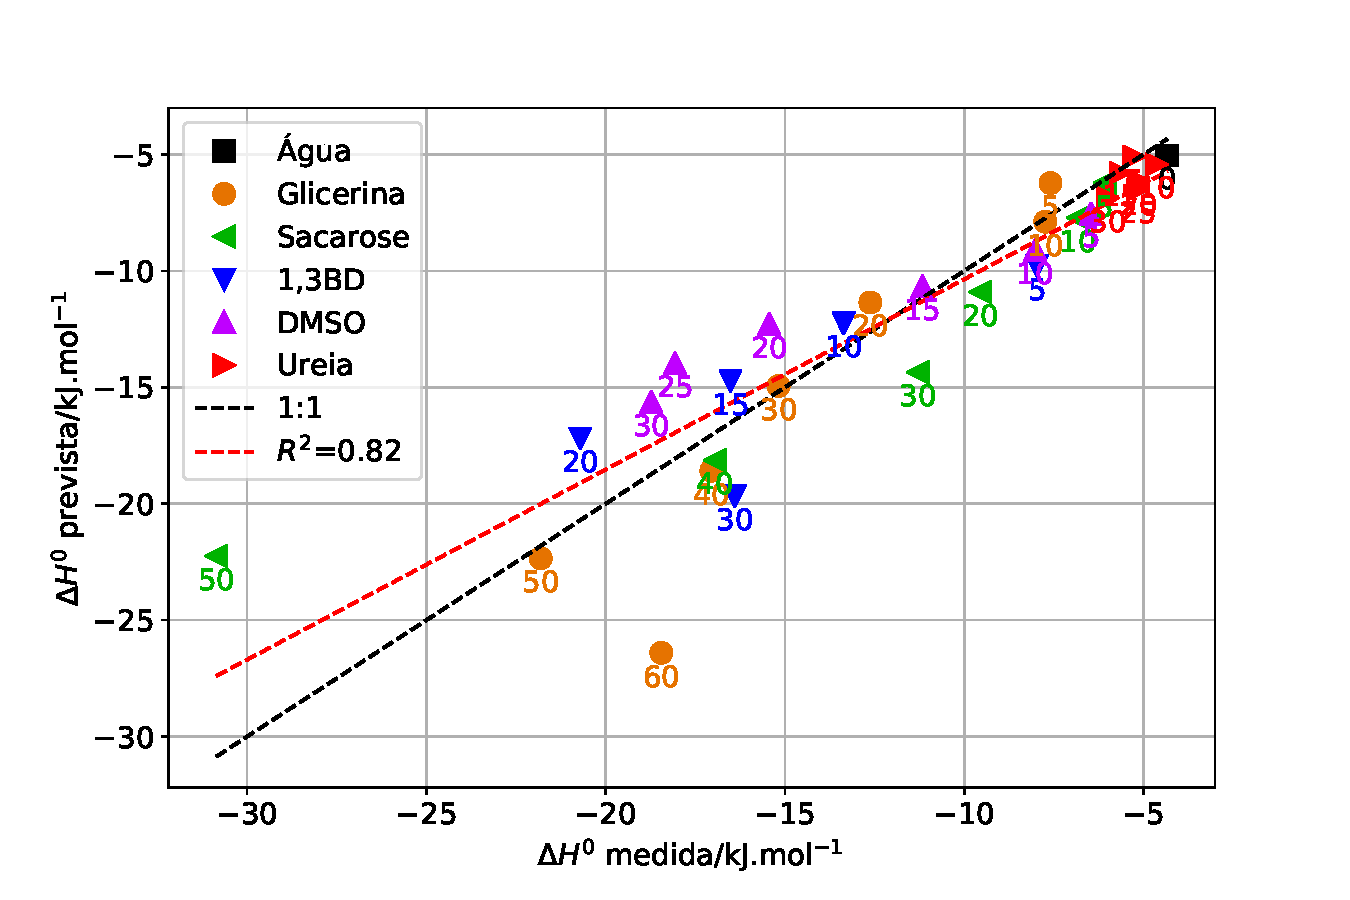
\includegraphics[width=0.7\textwidth]{imagens/itc/ols_dh_python}
			\caption{Comportamento do modelo de \DHmic{} criado por OLS, mostrando a correlação entre os valores observados e previstos. A reta preta tracejada o modelo perfeito, onde há uma relação 1:1 entre o observado e o previsto. A reta vermelha mostra o modelo criado, junto com a qualidade do ajuste.}
			\label{fig:ols_dh_python}
		\end{figure}

		Para realizar as análises e criar a figura \ref{fig:ols_cmc_python}, utilizou-se o código \ref{lst:ols_cmc_python}.
		
		\begin{listing}[h]
			\inputminted{python}{./python/ols_cmc_statsmodels.py}
			\caption{Código utilizado para gerar a dependência de \cmc{} com os parâmetros estudados, resultando na Fig. \ref{fig:ols_cmc_python}. A tabela de dados utilizada possui em cada linha as misturas utilizadas, suas concentrações em \% m/m, as variáveis dependentes (\cmc{} e \DHmic) e as variáveis independentes (\(n\), \(\varepsilon\), \(G\)).}
			\label{lst:ols_cmc_python}
		\end{listing}
		
		Os modelos obtidos estão nas equações \ref{eqn:ols_cmcs} e \ref{eqn:ols_dhs}. O pacote fornece os parâmetros autoescalados, e para convertê-los em parâmetros nas unidades tradicionais, é necessário desescalá-los, o que pode ser feito com o código da listagem \ref{lst:ols_cmc_conversao}.
		
		\begin{subequations}
			\begin{align}
			\textrm{CMC}               & = -7,073G              + 0,239\varepsilon             + 43,5n              -54,67  \label{eqn:ols_cmc}     \\
			\textrm{CMC}_{\textrm{AS}} & = -0,917G_\textrm{AS}  + 0,919\varepsilon_\textrm{AS} +0,497n_\textrm{AS}          \label{eqn:ols_cmc_AS}
			\end{align}
			\label{eqn:ols_cmcs}
		\end{subequations}
		
		\begin{subequations}
			\begin{align}
			\Delta H_\textrm{mic}^0     & = 6,29G              + 0,372\varepsilon             - 138n               + 132  \label{eqn:ols_dh} \\
			\Delta H_\textrm{mic, AS}^0 & = 0,258G_\textrm{AS} + 0,432\varepsilon_\textrm{AS} - 0,480n_\textrm{AS}        \label{eqn:ols_dh_AS}
			\end{align}
			\label{eqn:ols_dhs}
		\end{subequations}
		
		\begin{listing}[h]
			\inputminted{python}{./python/ols_cmc_conversão.py}
			\caption{Código utilizado para transformar os parâmetros dos ajustes de autoescalados para valores habituais.}
			\label{lst:ols_cmc_conversao}
		\end{listing}
		
		Ambos os conjuntos de equações são bastante semelhantes, o que mostra que é possível realizar essas correlações tanto com o método mais complexo (PLS) quanto o método mais simples (OLS). Como o número de parâmetros utilizado é pequeno, é recomendado utilizar o método mais simples. % todo: checar o livro da Márcia e o que ele fala sobre isso.
		
		Assim como nas equações \ref{eqn:PLS_cmcs} e \ref{eqn:PLS_dhs}, os coeficientes dos parâmetros estão relacionados com o quanto cada parâmetro afeta os processos. Os sinais são iguais, logo as interpretações são as mesmas.
		
		Ambos os modelos apresentados possuem validade somente para os mesmos aditivos, nas faixas empregadas. Não há garantia de que esses modelos consigam prever outros aditivos, a não ser que parâmetros adicionais, mais gerais, sejam propostos.
		
		Além disso, os parâmetros escolhidos não são necessariamente independentes, ou seja, não são ortogonais. Isso diminui a qualidade dos modelos criados. Porém, o motivo principal para a criação desses modelos foi tentar interpretar o conjunto de informações simultaneamente, o que é difícil pois o conjunto de dados possui 5 dimensões. Logo, o objetivo desse estudo foi cumprido.% todo: encontrar a relação de eps e n.
		
		Foram feitas correlações dos parâmetros com as propriedades das micelas gigantes, porém os ajustes foram muito ruins. Isso se deve provavelmente à maior complexidade do sistema, devido à presença de NaSal, e não é possível explicar as variações considerando-se somente três parâmetros.
		
		
		\FloatBarrier
		
		\section{Visualização das semelhanças dos solventes}
		
		Uma maneira de visualizar a similaridade das misturas binárias é utilizando um dendrograma. Esse tipo de gráfico é produzido calculando-se a distância entre pontos. Neste caso, cada ponto, representando cada mistura, está em um espaço tridimensional, de coordenadas \(n\), \(\varepsilon\) e \(G\). Inicialmente, calcula-se a distância entre os pontos, e agrupa-se os pontos que forem mais próximos, e repete-se o cálculo de distância, agora entre os grupos. O método de cálculo para a distância entre grupos varia, podendo ser feito, por exemplo, pelo ponto médio ou pela média das distâncias de todos os pontos. % todo: a completa é essa última descrita?
		
		Dito isso, foi montado um dendrograma das misturas binárias, que está presente na figura \ref{fig:dendrograma}. Do lado esquerdo do gráfico, os solventes estão sendo vistos com grande ``criteriosidade'', onde pequenas diferenças conseguem separá-los. À medida que se anda para a direita, a lupa se afasta e os solventes começam a se agrupar, até que todos os solventes são vistos como um só. A reta vertical simboliza o ponto onde a semelhança entre as misturas é de 50\%. Nessa região, os solventes podem ser separados em 6 grupos distintos, que foram coloridos.
		
		\begin{figure}[h]
			\centering
			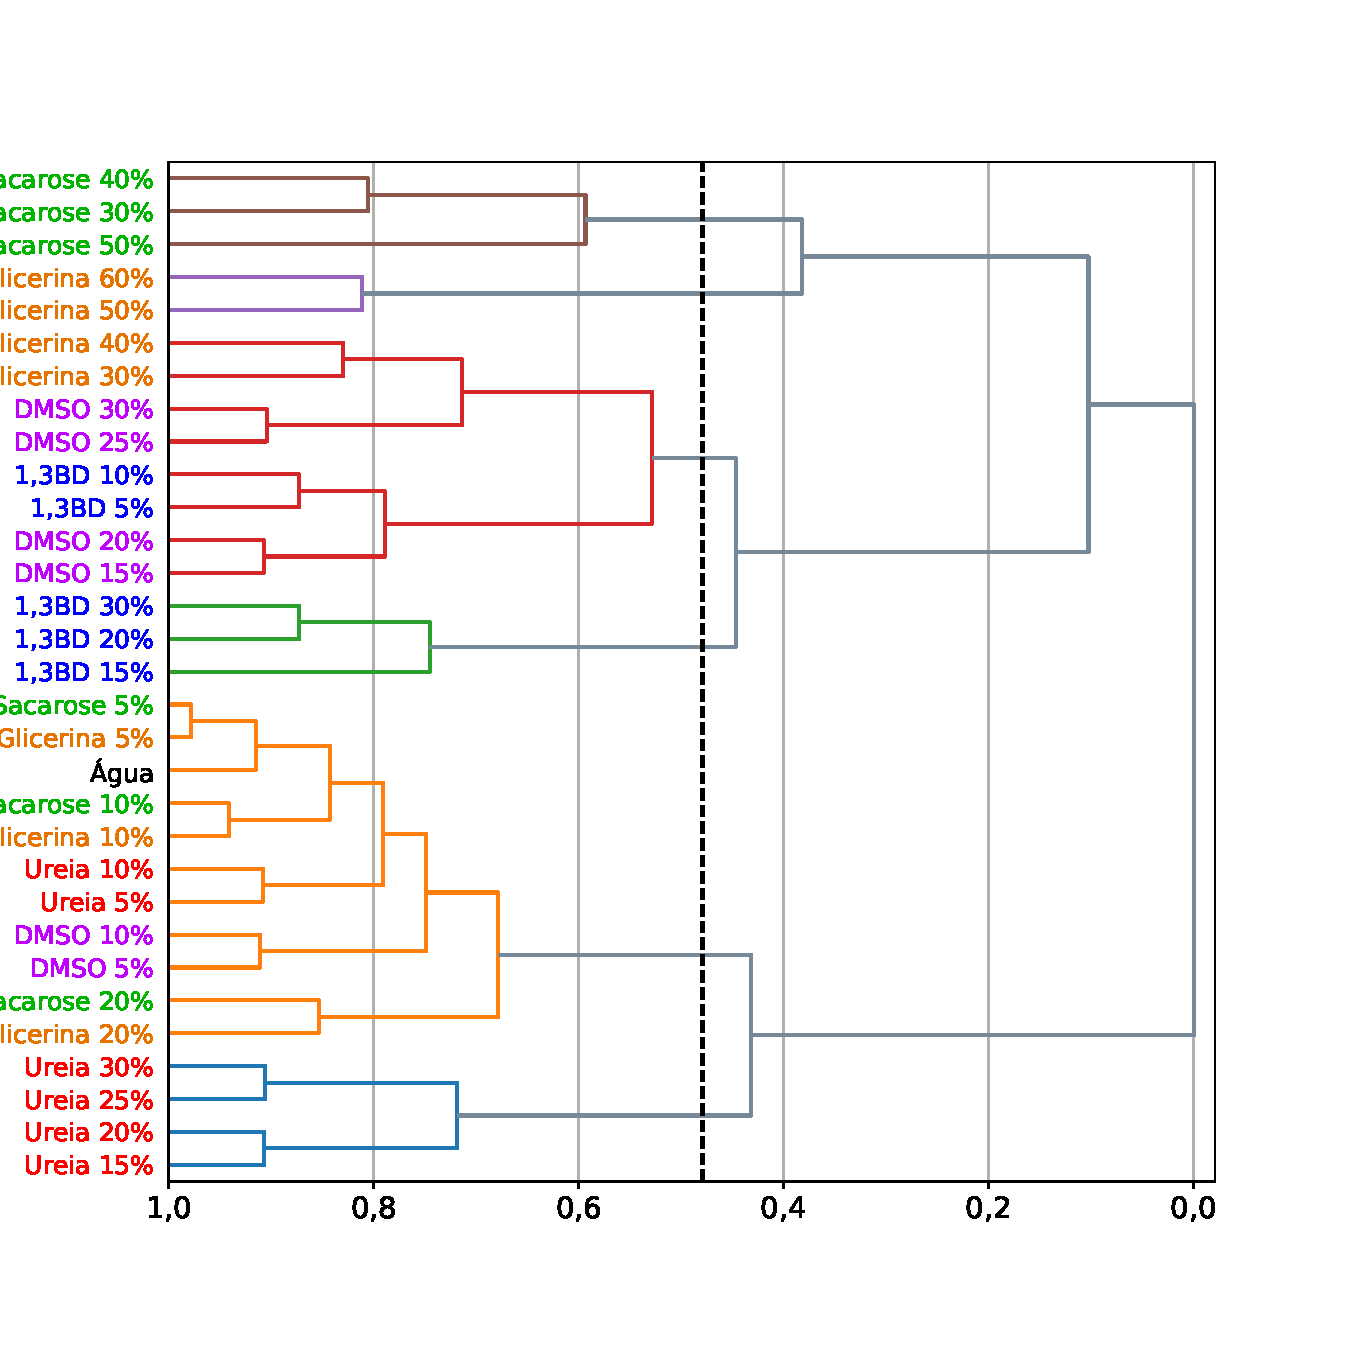
\includegraphics[width=0.7\textwidth]{imagens/propriedades/dendrograma}
			\caption{Dendrograma das propriedades das misturas binárias. A tabela de propriedades utilizada para esse gráfico é a mesma utilizada para os ajustes}
			\label{fig:dendrograma}
		\end{figure}
		
		Podemos observar a clara divisão entre dois grupos maiores. Um deles, acima, contém todas as misturas com alta concentração de aditivo, e todas as misturas de 1,3BD. Abaixo, temos todas as misturas de baixa concentração de aditivo, e todas as de ureia. Dentro do grupo da alta concentração, podemos observar que a sacarose se ajunta, assim como a glicerina. Além disso, concentrações altas de glicerina se assemelham à concentrações um pouco menores de DMSO. 1,3BD em baixas concentrações é parecido com DMSO em concentrações moderadas, e 1,3BD em altas concentrações se isola.
		
		No grupo de baixa concentração, temos que as misturas de 5-10\% dos aditivos estão próximos, e que sacarose e glicerina 5\% são as mais próximas da água. Ureia em baixas concentrações afetou pouco as propriedades da solução, e se assemelha também à esses compostos, mais do que DMSO 5-10\%. O resto das concentrações de ureia se assemelham à esse grupo, provavelmente se separando pela constante dielétrica, e se mantendo próximos pelo índice de refração e parâmetro de Gordon.
		
		Para criar esse dendrograma, utilizou-se o código da listagem \ref{lst:dendrograma}.
		
		\begin{listing}[h]
			\inputminted{python}{./python/dendrograma.py}
			\caption{Código utilizado para criar o dendrograma da figura \ref{fig:dendrograma}}
			\label{lst:dendrograma}
		\end{listing}
		\FloatBarrier
%		\section{Decomposição em propriedades fundamentais}
%		TODO

		\section{Conclusão Parcial}
		
		Nesta parte do trabalho, mostrou-se o efeito de diversos aditivos na reologia e na calorimetria de micelas gigantes. Os experimentos reológicos mostraram como a cinética dos processos de relaxação foi afetada pela adição dos aditivos, e por calorimetria observou-se a espontaneidade de formação de micelas gigantes.
		
		Todos os aditivos estudados tiveram efeitos diferentes nas micelas gigantes. Por um lado, sacarose praticamente não afetou tanto a reologia quanto a formação das micelas gigantes, apesar de promover a formação de micelas esféricas. Por outro lado, 1,3-butanodiol diminuiu fortemente a viscosidade das micelas, porém afetou a formação tanto quanto os outros aditivos. Ureia se mostrou o aditivo mais diferente de todos, aumentando a viscosidade da região de equimolaridade e diminuindo nas outras. Glicerina e DMSO tiveram efeitos semelhantes, tanto diminuindo a viscosidade das micelas quanto sua espontaneidade de formação, com DMSO tendo um efeito um pouco mais forte que glicerina.
		
		% todo: por ref
		Para explicar esses fenômenos, considerou-se alguns parâmetros. Primeiramente, o índice de refração, levantado por Hoffmann e Abdel-Rahem, constante dielétrica, levantado por Abdel-Rahem, e parâmetro de Gordon, levantando também por Abdel-Rahem, mas aplicado somente para micelas esféricas. Combinando-se esses parâmetros com efeitos mais qualitativos, como a posição dos aditivos nas micelas, foi possível explicar bastante os fenômenos observados. O parâmetro com maior correspondência com o comportamento reológico foi o parâmetro de Gordon, relacionado à estruturação do solvente. Quanto mais próximo era o parâmetro de Gordon do solvente ao parâmetro da água pura, menos afetado era o diagrama de viscosidade. Isso pode se dever ao aditivo facilitar a movimentação das micelas durante seu processo de relaxação, desestruturando o solvente. A exceção é ureia, pois é o único aditivo que aumenta a constante dielétrica do meio, e então remove espécies carregadas, como \Sal, da superfície micelar, aumentando a quantidade de \Sal{} necessária para atingir a neutralidade de carga. A interação dos aditivos com a superfície micelar deve ser considerada também, pois 1,3-butanodiol pode agir como um cosurfactante de cadeia curta, diminuindo o tempo de relaxação das micelas, diminuindo sua viscosidade.
		
		As calorimetrias de formação de micelas gigantes foram afetadas pelo solvente. Todos os solventes, com exceção de sacarose, aumentaram a concentração de formação de micelas gigantes, \cwlm, por uma combinação dos efeitos levantados. O parâmetro de Gordon diminui a penalidade entrópica do solvente, desfavorecendo agregação. O aumento da constante dielétrica aumenta a dissociação de espécies, aumentando a repulsão, também levando ao desfavorecimento da agregação. O índice de refração está relacionado à atração das moléculas de surfactante, e quanto maior for o índice, menor é a atração e menor é a tendência de formação micelar.
		
		De modo a observar o efeito de todos os parâmetros simultaneamente, foram realizados ajustes para se obter equações empíricas relacionando os parâmetros às propriedades. Foi possível correlacionar somente as concentrações micelares críticas (\cmc) e entalpias de micelização (\DHmic) aos parâmetros escolhidos. Isso ocorreu possivelmente pela maior simplicidade do sistema sem NaSal.
		
		Como perspectivas futuras, pode-se estudar outros aditivos para verificar o quanto os parâmetros levantados conseguem explicar outros comportamentos. Além disso, quantificar a concentração de aditivo na superfície micelar, mostrar como esses aditivos interagem com as moléculas de surfactante, com as moléculas de salicilato, e seus efeitos na cinética de quebra e recombinação micelar aprofundariam o entendimento sobre micelas gigantes. Frequentemente micelas gigantes são empregadas em produtos de cuidados pessoais que possuem uma grande quantidade de aditivos, logo entender como esses aditivos afetam as micelas é de grande interesse comercial. Por exemplo, 1,3-butanodiol é um aditivo utilizado comercialmente como XYZ, porém se adicionado à uma formulação de xampu, notaria-se uma queda considerável na viscosidade, o que pode ser explicado pelos efeitos do 1,3BD no solvente e nas micelas.
		
		%Além disso, seria interessante, com a ajuda de especialistas, desmembrar os parâmetros levantados em componentes mais fundamentais, necessariamente ortogonais, o que removeria problemas de interferência de um parâmetro nos outros.
		
		% todo: criar correlações agora utilizando outros parâmetros para índice de refração e cte dielétrica. Utilizar, por exemplo, (\varepsilon_r - 1 )/(2 \varepsilon_r + 1) e refração molar (V_m (n^2 - 1)/(n^2 - 2)) e cte dielétrica x dipolo, energia coesiva (raiz quadrada do param de hildebrand)
		% todo: tentar correlacionar viscosidades utilizando os parâmetros, mais a conc de salicilato como variáveis independentes
		% todo: ler livro do Reichardt, Welton